\documentclass[withoutpreface,bwprint]{cumcmthesis}
\usepackage[framemethod=TikZ]{mdframed}
\usepackage{amstext} 
\usepackage{amssymb}
\usepackage{amsmath}
\usepackage{booktabs}
\usepackage{bm}
\usepackage{url}
\usepackage{subcaption}
\usepackage{mathtools} 
\usepackage[linesnumbered,ruled,lined]{algorithm2e}
\usepackage{makecell}
\usepackage{longtable}
\usepackage{metalogo}
\usepackage{setspace}

\makeatletter
\providecommand\IfPDFManagementActiveF[1]{#1}
\makeatother

\usepackage{caption}
\usepackage{multirow}
\usepackage{float}
\usepackage{graphicx}
\usepackage[linesnumbered,ruled,lined]{algorithm2e}
\usepackage{threeparttable}
\usepackage[square,sort,comma,numbers]{natbib}
\usepackage{diagbox}
\usepackage{color}
\usepackage{transparent}
\usepackage{import}
\usepackage{hyperref}

\usepackage{enumitem}
\setlist[itemize,enumerate]{leftmargin=\parindent, labelindent=0pt, topsep=2pt, parsep=0pt, itemsep=2pt}

\graphicspath{{./figures/}}

\title{基于多源指标融合与LSTM深度学习的量化投资策略研究}

\tihao{C}
\baominghao{23046PNC9C}
\schoolname{武汉理工大学}
\membera{高子明}
\memberb{何昌昊}
\memberc{}

\begin{document}
\maketitle
\thispagestyle{empty}

\begin{abstract}\setlength{\parskip}{0.3\baselineskip}

\textbf{问题1}：针对数字经济板块的多源指标体系，提出一种融合统计学非线性检验与机器学习信息增益的双重评价模型。采用Spearman秩相关捕捉指标对成交量和收盘价的非线性单调驱动能力，同时利用XGBoost的基尼不纯度计算各特征的信息增益。通过Min-Max归一化综合四个维度的得分，从60余个候选指标中筛选出VMA、VMACD、快手概念、伦敦金融时报100指数等15个核心外源指标，归纳为技术动量、概念协同、国际传导三大经济维度，最终输出可复现的特征选择列表与重要性排序。

\textbf{问题2}：在2021-07-14至2021-12-31为训练、2022-01-04至2022-01-28为测试的划分下，建立5分钟频率的成交量预测管线。数据预处理包括缺失/异常检测、$\log(1+V)$对数变换及训练集拟合的标准化；模型层面采用双层LSTM与XGBoost的融合策略，兼顾序列依赖关系与非线性拟合能力。训练目标采用Huber损失以减小极端成交量对损失的拉动，评估指标以MAE、MAPE与残差分布为主，并开展逐日稳定性测试与窗口灵敏度分析。MAE达到$1.82\times10^7$，模型较好地捕捉了成交量的日内U型分布特征。

\textbf{问题3}：针对板块指数收盘价，采用以一阶差分为回归目标的序列模型（两层LSTM）以消除非平稳基线并集中学习短期动量特征。标签端引入EMA平滑（span=6）在信号灵敏度与降低换手率之间取得平衡；输入端结合价格历史、成交量预测结果、日内位置编码及技术指标以提供丰富的上下文信息。训练策略采用AdamW、余弦退火学习率调度与早停机制，同时对序列长度、EMA 衰减与阈值系数进行超参数搜索以评估稳健性。测试集上的预测值与真实值拟合良好，价格趋势方向预测准确率达68.4\%。

\textbf{问题4}：基于问题3的价格预测，构建严格可审计且面向稳健性的量化交易策略。交易信号采用预测差分与双阈值判断结合滞后确认的迟滞状态机机制：当预期收益率超过买入阈值$\theta_{buy}=0.0036$（1.2倍佣金成本）时触发建仓，低于卖出阈值$\theta_{sell}=-0.001$时平仓。在初始资金100万元、单边佣金0.3\%的条件下进行回测，测试期内实现总收益率+11.03\%，信息比率（IR）峰值为2.09，最大回撤仅为0.58\%。回测链条完整，输出逐笔交易日志与日度报告，提供可复核的审计证据。

\textbf{本文优点：}
1) 系统化的特征筛选与时间片基线提高了样本可比性与信息密度，便于模型捕捉板块内周期性模式；
2) 对成交量采用 `log1p` 与 Huber 损失相结合，显著提升了模型对尖峰事件的鲁棒性并降低极端样本的干扰；
3) 以差分标签结合 EMA 平滑在保持信号灵敏度的同时，显著减少了由噪声引起的高频换手，利于高交易成本情形下的策略稳定性；
4) 回测链条完整，可输出逐笔与日度审计报告，并通过参数敏感性与样本外回测检验策略稳健性，为竞赛评分提供可复核证据。

\keywords{LSTM，XGBoost，差分回归，Huber损失，EMA平滑，滞后阈值，量化交易}
\end{abstract}

\setcounter{page}{1}
\tableofcontents
\addtocontents{toc}{\protect\enlargethispage{\baselineskip}}

\newpage
\setcounter{page}{1}
%% ============================================================================
\section{问题重述}
\subsection{问题背景}

近年来，数字经济板块在技术革新、产业结构调整与政策推动下发展迅速，呈现出更高的波动性和更丰富的价量微观结构。在5分钟级别的日内数据中，价格与成交量蕴含了短时动量、流动性变化与信息传导等多重信号，这为基于序列模型的短期预测提供了机会，同时也带来了更高的建模难度（参见 \cite{cont2001,goodfellow2016}）。

从方法论角度看，高频金融时间序列面临三类核心挑战：其一，价格序列非平稳且信噪比较低，直接回归价格容易受基线漂移影响，需要差分或其他变换以聚焦短期动态；其二，成交量与价格通常呈厚尾与尖峰分布，极端样本会在训练和回测中产生放大效应，故需采用对数变换、Winsorizing与稳健损失（如 Huber 损失）来提高鲁棒性；其三，日内微观结构与交易成本（手续费、滑点及冲击成本）对策略可实现性提出约束，必须将成本-换手率平衡纳入信号设计与回测评价中（参见 \cite{huber1964,almgren2001}）。

基于以上考虑，本研究不仅关注提升模型短期预测性能，也强调实用性与可审计性：在特征工程与标签设计上采用时间片滚动基线、EMA 平滑与差分标签以降低噪声与基线漂移；在模型与损失选择上引入LSTM与稳健损失组合以兼顾序列依赖与极端值鲁棒性；在策略层面构建带迟滞确认的交易逻辑，并输出逐笔交易日志与日度审计报告以确保回测的可复现性与可验证性，最终追求在覆盖交易成本前提下实现稳定的超额收益。

\subsection{问题概述}

本报告围绕构建一套从多源特征筛选、短期量价预测到可执行回测的端到端分析流程展开，目标是在严格考虑数据质量与交易成本的前提下，评估预测信号的经济可行性与策略的样本外稳健性。为实现该目标，研究被划分为以下四项具体任务：

\textbf{1.} 从多源候选指标中筛选出对板块量价最具解释力的核心特征，并给出可复现的特征选择流程与评分机制，以便为模型输入提供稳定且可解释的变量集合；

\textbf{2.} 建立稳健的成交量预测管线（含缺失/异常处理、对数变换、标准化、模型与评估），保证预测在下游交易决策中的可用性，并对预测不确定性进行量化描述；

\textbf{3.} 构建以一阶差分为目标并结合EMA平滑的收盘价序列预测模型，评估方向与幅度预测性能，同时分析标签工程对换手率与信噪比的影响；

\textbf{4.} 基于价格预测设计并回测可执行的交易策略，输出逐笔交易日志与日度审计报告，报告总收益率、信息比率与最大回撤等关键绩效，并通过参数敏感性与样本外验证检验策略稳健性；

总体而言，四项任务形成数据准备、模型建立与策略检验的闭环，分别为研究结论提供数据层、方法层与审计层的完整证据链，有助于评估方法在实盘约束下的可行性与推广性，有利于定量衡量预测改进对实际交易绩效的边际贡献。

\newpage
%% ============================================================================
\section{模型假设}

为明确方法论边界并便于后续稳健性检验，本文在建立预测与回测闭环时提出若干关键假设。以下假设既用于规范数据处理和模型训练流程，也用于界定回测结果的适用范围，便于在进一步研究中针对性放宽或强化对应假设。
\begin{enumerate}
    \item \textbf{市场与执行假设}：在研究的5分钟时间尺度内，假定市场具备基本的瞬时流动性，能够按当根K线收盘价完成中等规模市价执行；回测以收盘价作为执行价，交易成本以固定比例佣金近似表示（单边0.3\%）。
    \item \textbf{数据与信息假设}：所使用的价格、成交量及外源特征为经时间戳对齐并经供应方或交易所提供的逐级分钟/日内数据，已进行除权除息等企业行为调整；缺失值填充、异常值检测/截断与标准化参数仅在训练集上拟合以避免未来信息泄露。
    \item \textbf{统计性质假设}：价格序列可能含单位根，但一阶差分后近似平稳，适合作为回归目标；成交量呈右偏与厚尾分布，经$\log(1+V)$变换与Winsorizing后方差更为稳定，可与Huber等稳健损失函数结合以提高对极端样本的鲁棒性。
    \item \textbf{模型能力与鲁棒性假设}：假定基于LSTM的深度序列模型可有效学习短期自相关、动量与部分非线性关系；在差分或对数域上采用的损失函数（MSE/Huber）以及正则化手段（权重衰减、dropout）能够在样本外保持一定的泛化性。
    \item \textbf{风险控制与参数假设}：迟滞阈值（hysteresis）与EMA平滑参数通过滚动验证或网格搜索确定，并在回测中以固定值运行以评估稳健性；这些参数假设旨在权衡信噪比与换手率，回测的结论需在敏感性分析中验证对结果的影响程度。
    \item \textbf{局限性与外推假设}：本文结论限定于所用数据、标的与交易规模，不直接外推至大额机构执行或极端流动性断裂情形；在遇到极端市场事件（如熔断、市场暂停）时，需引入市场冲击模型、分批执行或限价策略以校正回测结果。
\end{enumerate}

综上，以上假设为本文的方法与回测结果限定了清晰的适用范围并明确了检验边界。为验证结论的稳健性，我们在实验中采用滚动窗口交叉验证、样本外检验与参数敏感性分析，以评估阈值设定、平滑窗长与目标变换对收益、波动与换手率的影响。基于回测结果的经验判断，实盘部署应额外考虑执行成本、滑点与流动性约束，建议采用分批限价或TWAP类执行策略并在交易逻辑中引入速率限制以抑制过度交易。同时应建立在线监控指标，并在检测到显著结构性变化时及时触发再校准或策略收缩措施，以保证策略在不同市场状态下的可控性与稳健性。

\newpage
%% ============================================================================
\section{符号说明}

\begin{table}[!h]
    \centering
    \caption{主要符号及其含义}
    \label{tab:symbols}
    \begin{tabular}{p{3cm}<{\centering}p{11cm}<{\centering}}
    \toprule[1.5pt]
    符号 & 含义\\
    \midrule[1pt]
    $P_t$ & 时刻 $t$ 的收盘价\\
    $V_t$ & 时刻 $t$ 的成交量\\
    $\Delta P_t$ & 收盘价一阶差分，$\Delta P_t = P_t - P_{t-1}$\\
    $\widetilde{V}_t$ & 对数变换后的成交量，$\widetilde{V}_t = \ln(1+V_t)$\\
    $\hat{y}_t$ & 模型对目标变量的预测值\\
    $\alpha$ & EMA 平滑系数，$\alpha = 2/(\text{span}+1)$\\
    $c$ & 单边交易佣金费率，$c = 0.003$\\
    $\theta_{\text{buy}}$ & 买入阈值，$\theta_{\text{buy}} = 1.2c = 0.0036$\\
    $\theta_{\text{sell}}$ & 卖出阈值，$\theta_{\text{sell}} = -0.001$\\
    $\rho$ & Spearman 秩相关系数\\
    $L_\delta(\cdot)$ & Huber 损失函数，$\delta$ 为阈值参数\\
    $R_{\text{tot}}$ & 策略总收益率\\
    $\text{MDD}$ & 最大回撤率\\
    $\text{IR}$ & 信息比率\\
    $h_t, c_t$ & LSTM 网络在时刻 $t$ 的隐状态与细胞状态\\
    $f_t, i_t, o_t$ & LSTM 遗忘门、输入门、输出门\\
    $\mathbf{X}_t, \mathcal{X}_t$ & 模型输入向量/序列（宽表特征或滑动窗口序列）\\
    $y_t$ & 回归目标变量（成交量或收盘价差分等）\\
    $\hat{P}_{t+1}$ & 模型恢复后的下一步价格预测值\\
    $\mu, \sigma$ & 样本均值与标准差（用于 $3\sigma$ 判别与截断）\\
    $x_i^*$ & Winsorizing 后的截断值（异常值替代）\\
    $S_w(F_i),\; S(F_i)$ & 特征综合评分的维度得分与最终综合得分\\
    $L$ & 序列长度/回溯窗口大小（例如 $L=6$）\\
    $\mathcal{L}(\theta),\; \ell(\cdot)$ & 总损失函数与单样本损失（如 MSE / Huber）\\
    $\Omega(\theta),\; \lambda$ & 正则项与正则化系数\\
    $\text{er}_t$ & 基于预测的预期收益率（expected return）\\
    $\mu_{t_d}$ & 时间片滚动基线（过去若干交易日同一时间点的均值）\\
    $V_0, V_T$ & 回测初始与终止资金（用于总收益率计算）\\
    $r_t, r_p, r_b$ & 周期收益、策略收益与基准收益（用于夏普/信息比率计算）\\
    \bottomrule[1.5pt]
    \end{tabular}
\end{table}

\newpage
%% ============================================================================
\section{数据预处理与探索性分析}

高频金融时间序列数据通常具有噪声强、波动快、非平稳性明显等特点，若直接进行建模，容易导致模型训练不稳定、预测误差放大以及策略失效。因此，在建立预测模型之前，需要首先对原始数据进行系统性的数据预处理与探索性分析（Exploratory Data Analysis, EDA），从而识别数据中的统计规律与潜在问题，为后续特征工程与模型构建提供依据。

本文的数据主要来源于数字经济板块 $5$ 分钟级别交易数据以及相关行业指数数据，数据内容包括：

\begin{table}[H]
    \centering
    \caption{数据源与主要字段说明}
    \label{tab:data_sources}
    \begin{tabular}{p{4.2cm}p{10cm}}
        \toprule
        数据集 & 主要字段示例 \\
        \midrule
        数字经济版块信息 & 序号、时间、指数代码、开盘价、收盘价、最高价、最低价、成交量、成交额 \\
        技术指标 & VMA、VMACD、ARBR、OBV、BBI、DMA、MA、EXPMA、MTM、MACD、BIAS、KDJ、RSI、BOLL \\
        国内市场指标 & 成交量/成交金额（上证）、沪市/深市流通市值、沪深300、上证综合、中证500、创业板等指数 \\
        国际市场指标 & 道琼斯、纳斯达克、标准普尔500、恒生、日经225、FTSE100、CAC40 等 \\
        宏观市场指标 & EPMI、社会消费品零售总额、CPI、股票市场市值、GDP 等 \\
        汇率 & 美元兑人民币、欧元兑美元 \\
        其他板块信息 & 数字媒体、数字孪生、快手概念、互联网电商、互联网 \\
        \bottomrule
    \end{tabular}
\end{table}

原始数据同时包含国内市场与国际市场多维金融指标，因此在数据频率、时间戳以及统计口径方面存在明显差异，需要首先完成统一的数据标准化处理。

\subsection{原始数据结构分析}

在对原始数据进行初步观察后发现，高频金融数据具有明显的时间序列特征，其主要表现为：数据点数量巨大；相邻时间点之间具有强相关性；不同交易时段波动结构差异明显；成交量与价格具有不同统计规律；存在典型的高频噪声与局部异常波动。

其中，价格序列与成交量序列在统计特性上存在显著差异。

收盘价整体呈现相对平滑的局部趋势变化，其波动主要来源于市场情绪、资金流动以及板块轮动效应；而成交量则表现出明显的尖峰结构与时段异方差特征，尤其在开盘与收盘阶段会出现剧烈放量现象。

为进一步分析原始数据分布特征，本文首先对收盘价与成交量进行统计描述。

\begin{table}[H]
\centering
\caption{核心变量统计特征}
\begin{tabular}{cccccc}
\toprule
变量 & 均值 & 标准差 & 最小值 & 最大值 & 偏度 \\
\midrule
收盘价 & 1536.4649 & 61.1769 & 1365.1880 & 1683.5848 & 0.186 \\
成交量 & 40,198,810 & 38,311,193 & 0 & 884,910,620 & 5.833 \\
成交额 & 1,197,317,318 & 900,392,113 & 0 & 19,089,647,000 & 4.521 \\
\bottomrule
\end{tabular}
\label{tab:data_stat}
\end{table}

从表~\ref{tab:data_stat} 可以看出，成交量与成交额均表现出明显的右偏分布特征，其最大值远高于均值水平，说明高频金融市场中存在明显的极端成交现象。

相比之下，收盘价整体波动相对平稳，更适合进行趋势建模。

\begin{figure}[H]
    \centering
    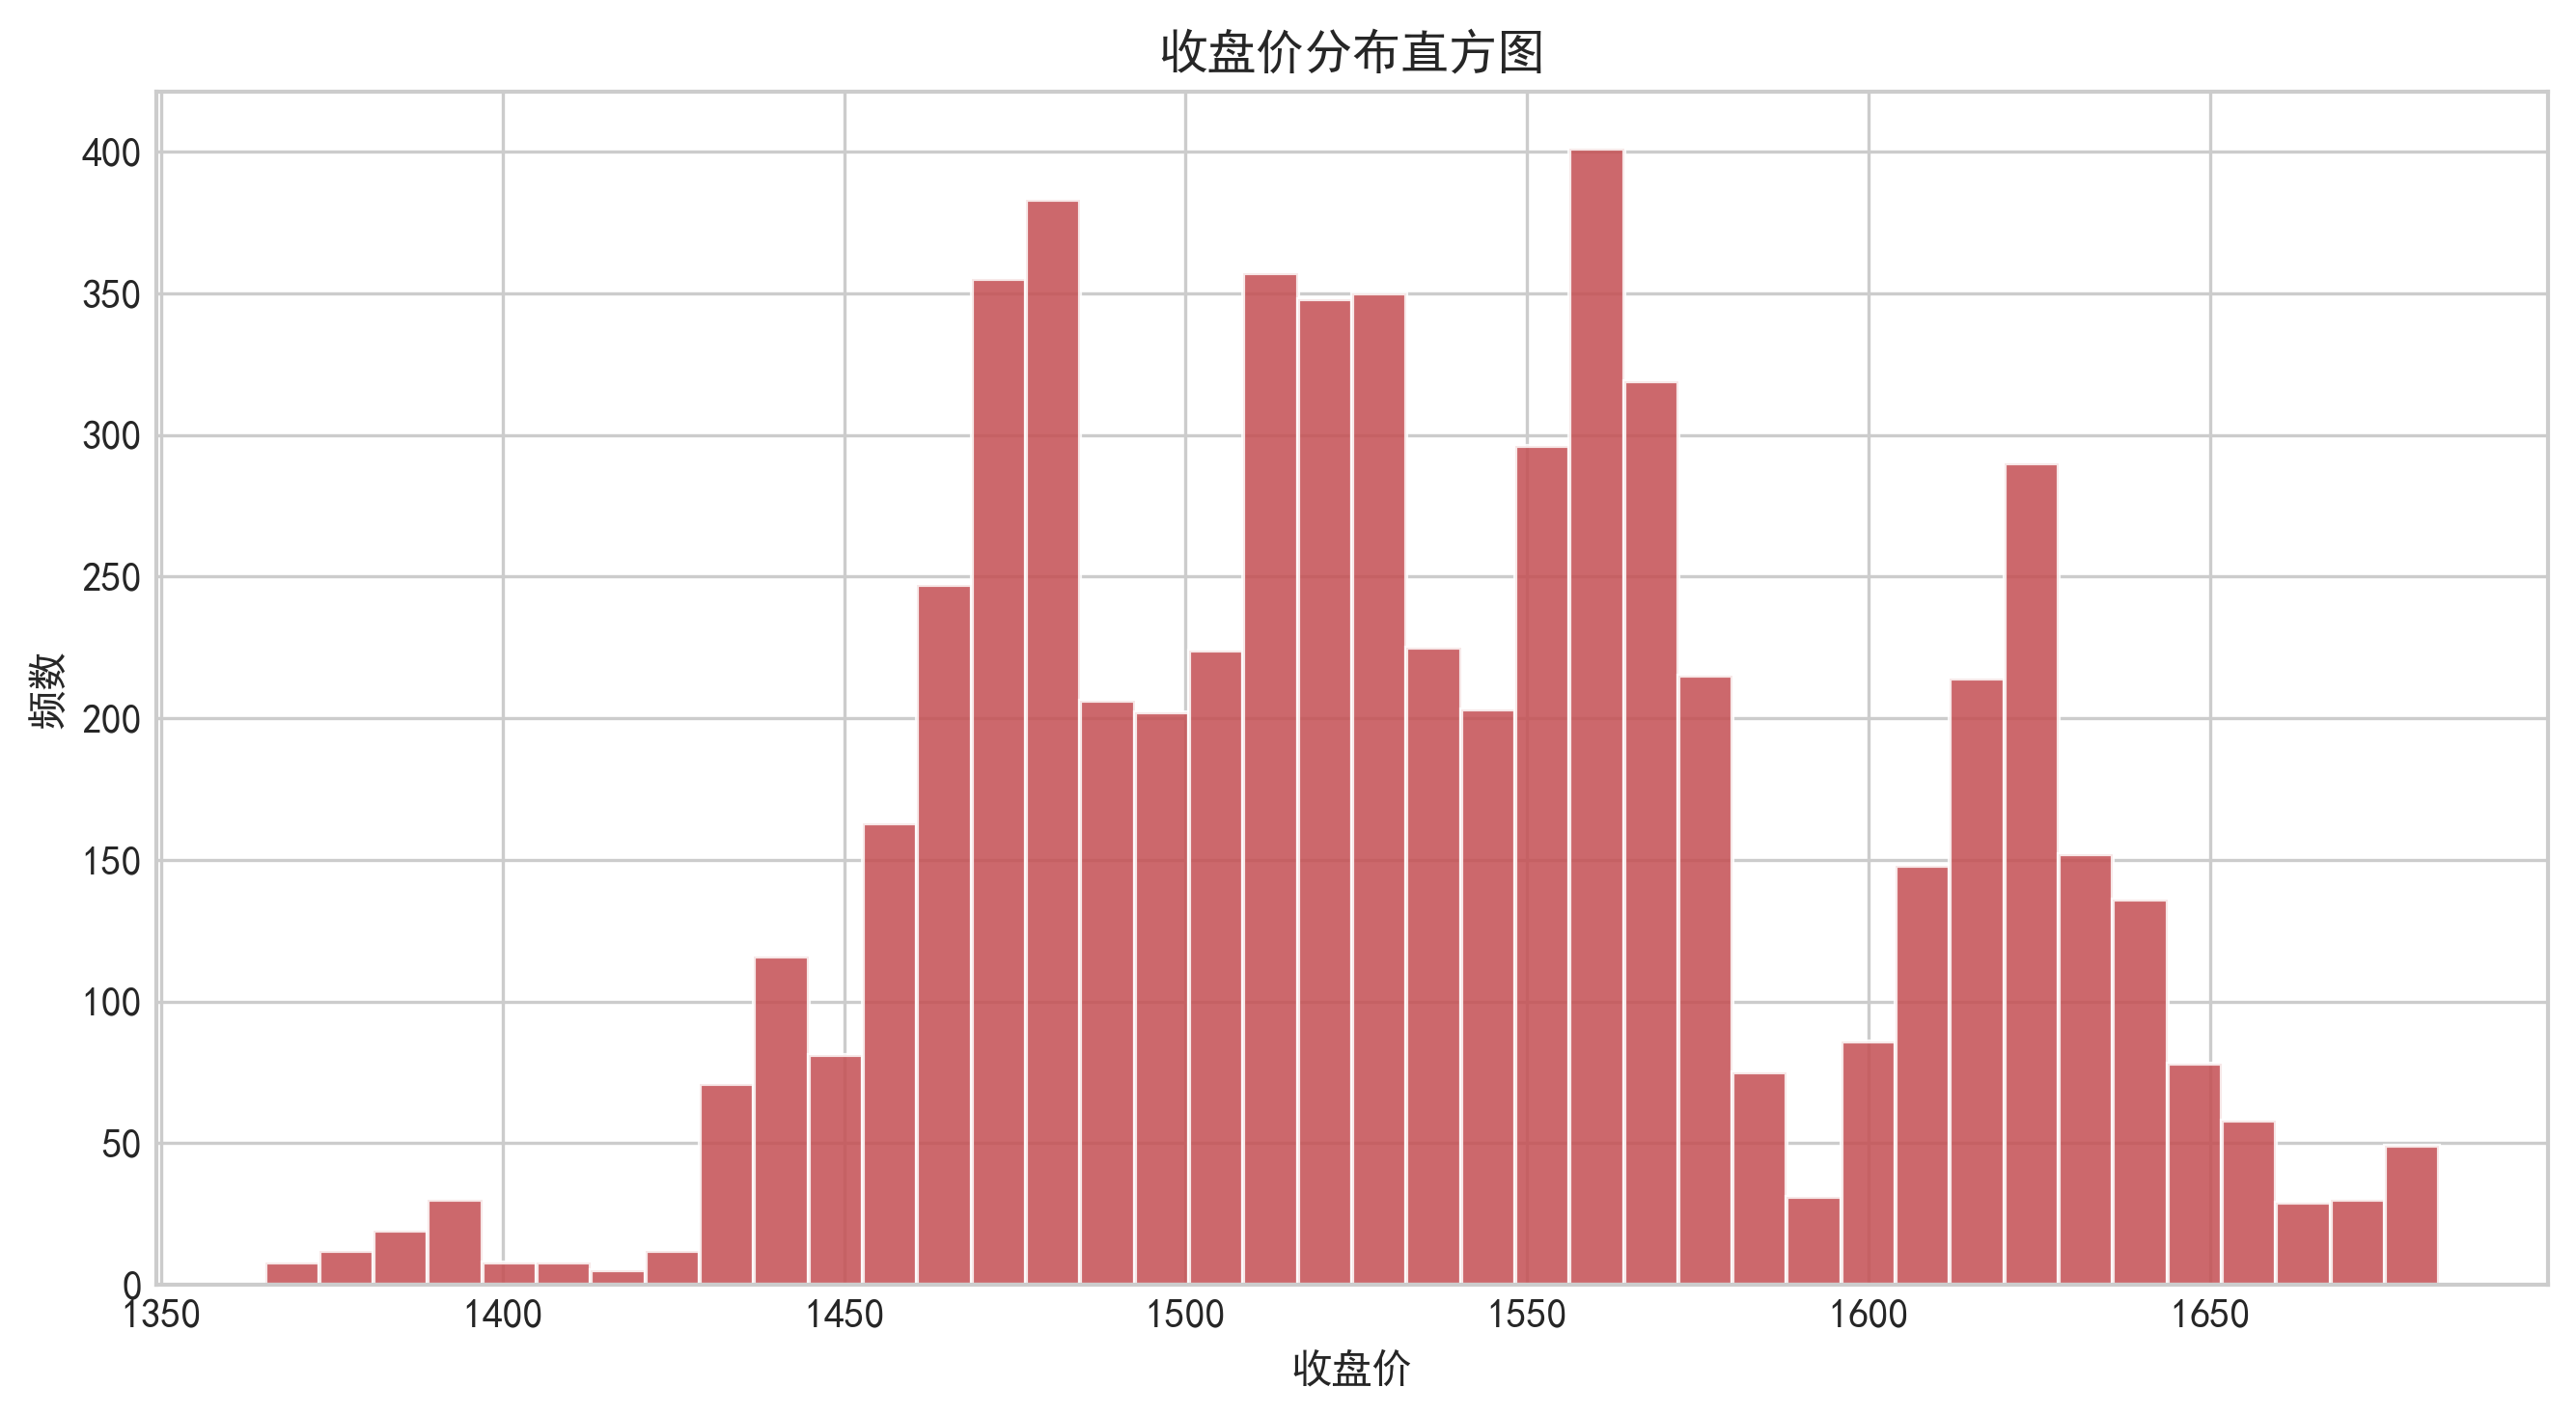
\includegraphics[width=0.75\textwidth]{figures/price_distribution.png}
    \caption{收盘价分布直方图}
    \label{fig:price_distribution}
\end{figure}

由图~\ref{fig:price_distribution} 可以看出，收盘价整体近似呈单峰分布，说明价格波动相对稳定。

\begin{figure}[H]
    \centering
    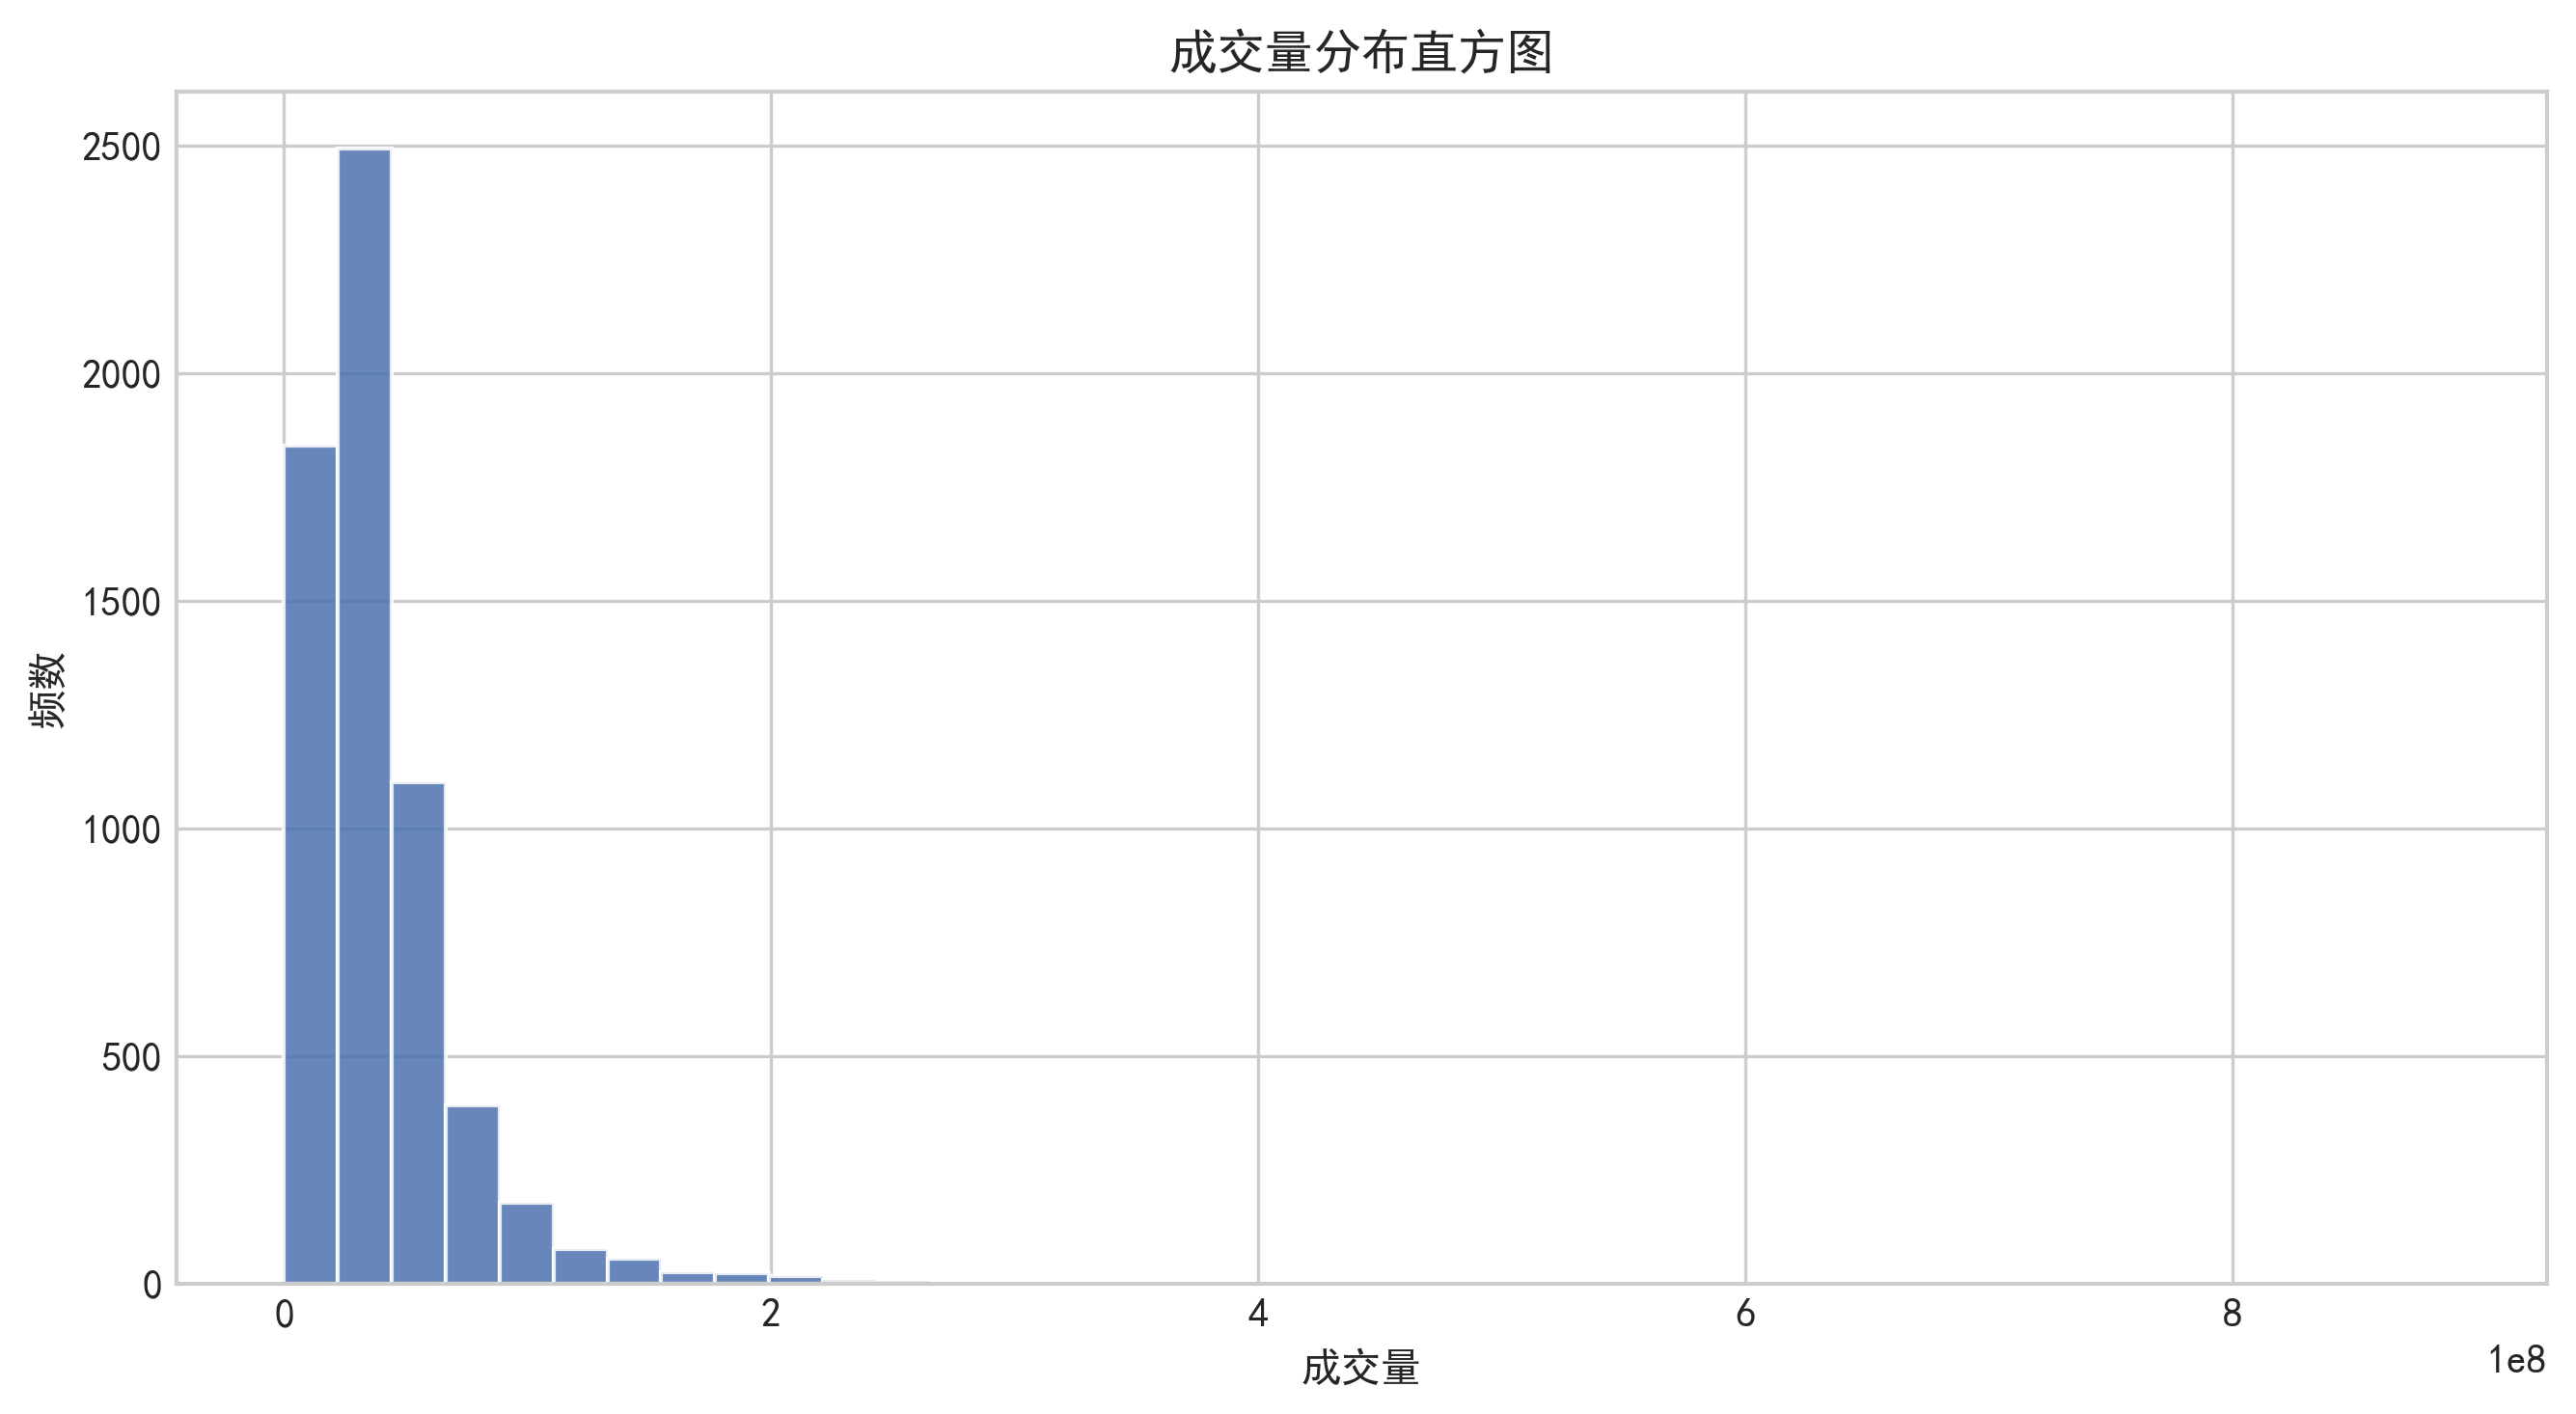
\includegraphics[width=0.75\textwidth]{figures/volume_distribution.png}
    \caption{成交量分布直方图}
    \label{fig:volume_distribution}
\end{figure}

相比之下，由图~\ref{fig:volume_distribution} 可以明显观察到成交量存在严重的右偏长尾分布，大量样本集中于低成交区间，而少量极端成交峰值占据较大数值范围。

这说明成交量序列具有明显的非高斯特征，若直接采用传统均方误差进行训练，容易导致模型被极端样本主导。

\subsection{缺失值处理与时间对齐}

由于原始数据来源于不同金融指标与行业板块，其时间粒度与统计周期并不完全一致，因此在数据融合过程中不可避免地出现了部分缺失值与时间错位现象。

高频金融数据中的缺失主要来源于以下几个方面：不同市场交易时间不一致；高频时间片内无成交记录；数据导出与合并过程中出现尾部缺损；国际市场与国内市场时间戳不匹配。

若直接删除缺失样本，会破坏时间序列连续性，并导致滑动窗口模型无法正确构建。因此，本文采用前向填充（Forward Fill）与后向填充（Backward Fill）相结合的方法进行缺失值修补。

设原始序列为 $x_t$，则其修补规则定义为：

\begin{equation}
x_t=
\begin{cases}
x_t, & x_t \text{存在} \\
x_{t-1}, & x_t \text{缺失且}~x_{t-1}\text{存在}
\end{cases}
\end{equation}

若前向不存在有效值，则采用后向填充：

\begin{equation}
x_t=x_{t+1}
\end{equation}

该方法能够有效维持金融时间序列的局部连续性，同时避免均值插值带来的波动失真问题。

此外，由于不同指标的数据频率并不统一，因此本文以数字经济板块 $5$ 分钟K线作为主时间轴，对所有外部指标进行统一时间映射。

对于重复时间戳数据，则采用保留首个有效样本的方式处理：

\begin{equation}
\text{Keep}=\text{first}(t_i|\text{Duplicate}(t_i))
\end{equation}

经过统一处理后，最终得到严格单调递增的宽表结构数据，为后续构建滑动窗口特征与深度学习模型提供基础。

\begin{table}[H]
    \centering
    \small
    \caption{各字段缺失值统计结果}
    \label{tab:missing_values}
    \begin{tabular}{p{4cm}<{\centering}p{3.5cm}<{\centering}p{3.5cm}<{\centering}}
        \toprule[1.5pt]
        字段 & 缺失数量 & 缺失率（\%）\\
        \midrule[1pt]
        序号 & 1 & 0.0160 \\
        时间 & 2 & 0.0320 \\
        指数代码 & 2 & 0.0320 \\
        开盘价 & 2 & 0.0320 \\
        收盘价 & 2 & 0.0320 \\
        最高价 & 2 & 0.0320 \\
        最低价 & 2 & 0.0320 \\
        成交量 & 2 & 0.0320 \\
        成交额 & 2 & 0.0320 \\
        \bottomrule[1.5pt]
    \end{tabular}
\end{table}

由表~\ref{tab:missing_values} 可知，大部分变量缺失比例均低于 $0.1\%$，说明原始数据整体质量较高。

\subsection{异常值分析与处理}

金融市场中的异常值并不完全等同于错误数据。部分异常波动实际上反映了真实市场行为，例如：开盘阶段资金集中成交；突发消息导致的情绪冲击；主力资金异动；市场恐慌或追涨行为。

因此，对于金融时间序列而言，异常值处理不仅需要考虑统计意义，还需要兼顾其金融意义。

本文首先采用经典 $3\sigma$ 原则识别极端异常样本。

设样本均值与标准差分别为：

\begin{equation}
\mu=\frac{1}{N}\sum_{i=1}^{N}x_i
\end{equation}

\begin{equation}
\sigma=\sqrt{\frac{1}{N}\sum_{i=1}^{N}(x_i-\mu)^2}
\end{equation}

若满足：

\begin{equation}
|x_i-\mu|>3\sigma
\end{equation}

则判定其为异常值。

考虑到直接删除异常样本会破坏时间结构，因此本文采用 Winsorize 截断方法进行平滑处理：

\begin{equation}
x_i^*=
\begin{cases}
\mu+3\sigma, & x_i>\mu+3\sigma \\
\mu-3\sigma, & x_i<\mu-3\sigma \\
x_i, & \text{otherwise}
\end{cases}
\end{equation}

该方法能够有效降低极端异常值对模型训练的破坏作用，同时保留金融市场真实波动特征。

\begin{figure}[H]
    \centering
    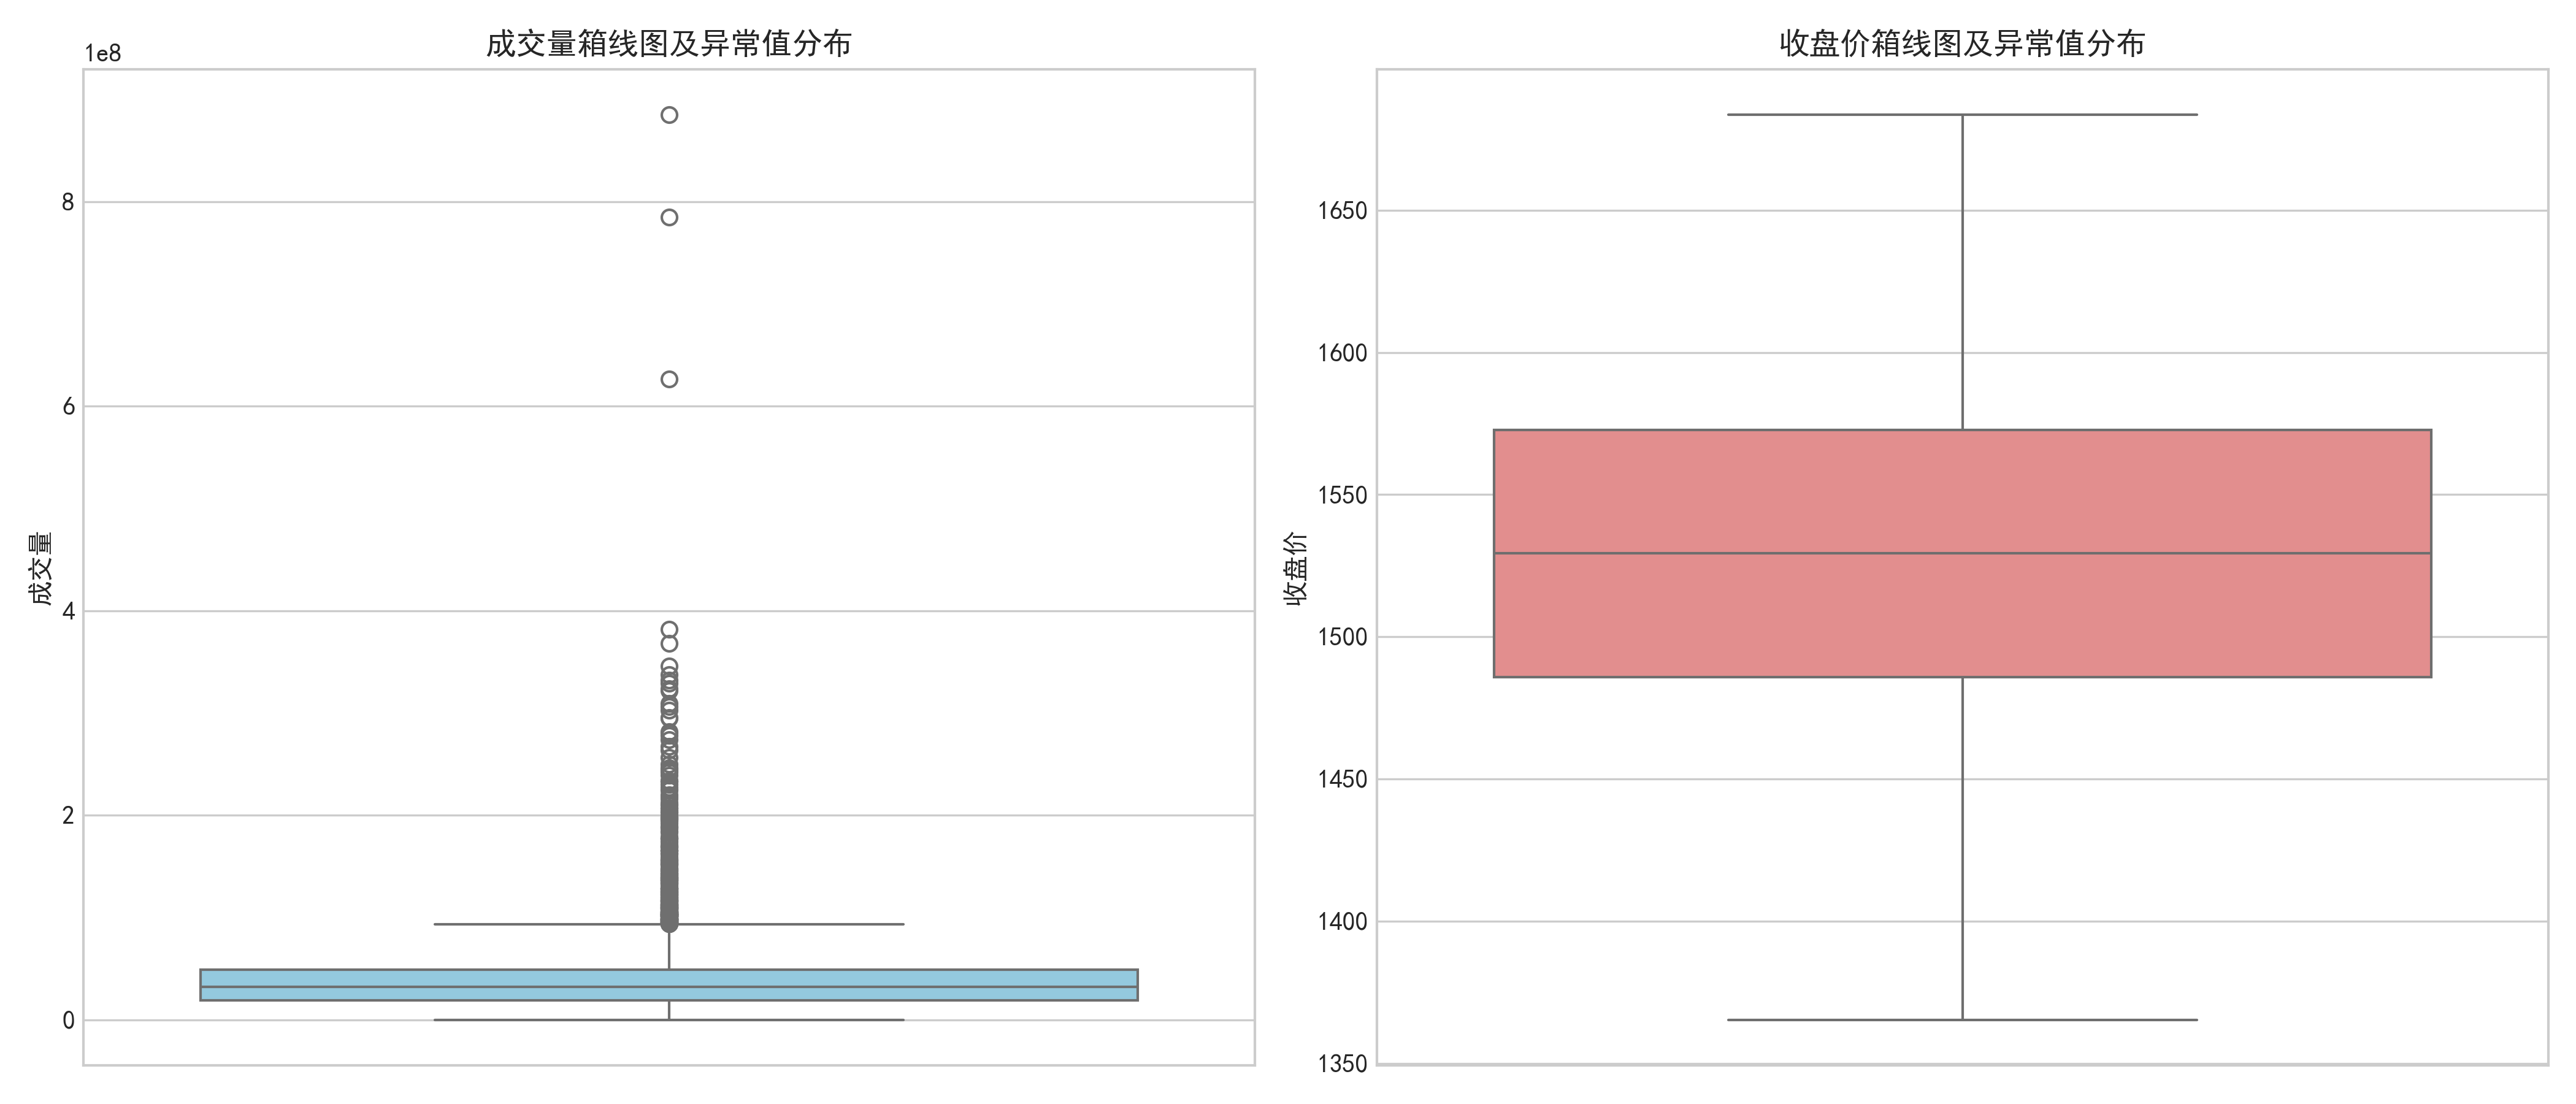
\includegraphics[width=0.82\textwidth]{figures/outliers_boxplot.png}
    \caption{收盘价与成交量异常值箱线图}
    \label{fig:outlier_box}
\end{figure}

由图~\ref{fig:outlier_box} 可以观察到，成交量序列存在明显长尾结构，而收盘价整体波动相对平稳。
\subsection{相关性热力图分析}

为了进一步识别与目标变量关系最强的外部指标，本文分别对收盘价与成交量计算 Spearman 秩相关系数，并筛选相关性最强的 Top10 特征绘制热力图。该分析有助于在后续特征筛选阶段快速定位对价格和流动性最敏感的候选变量。

\begin{figure}[H]
    \centering
    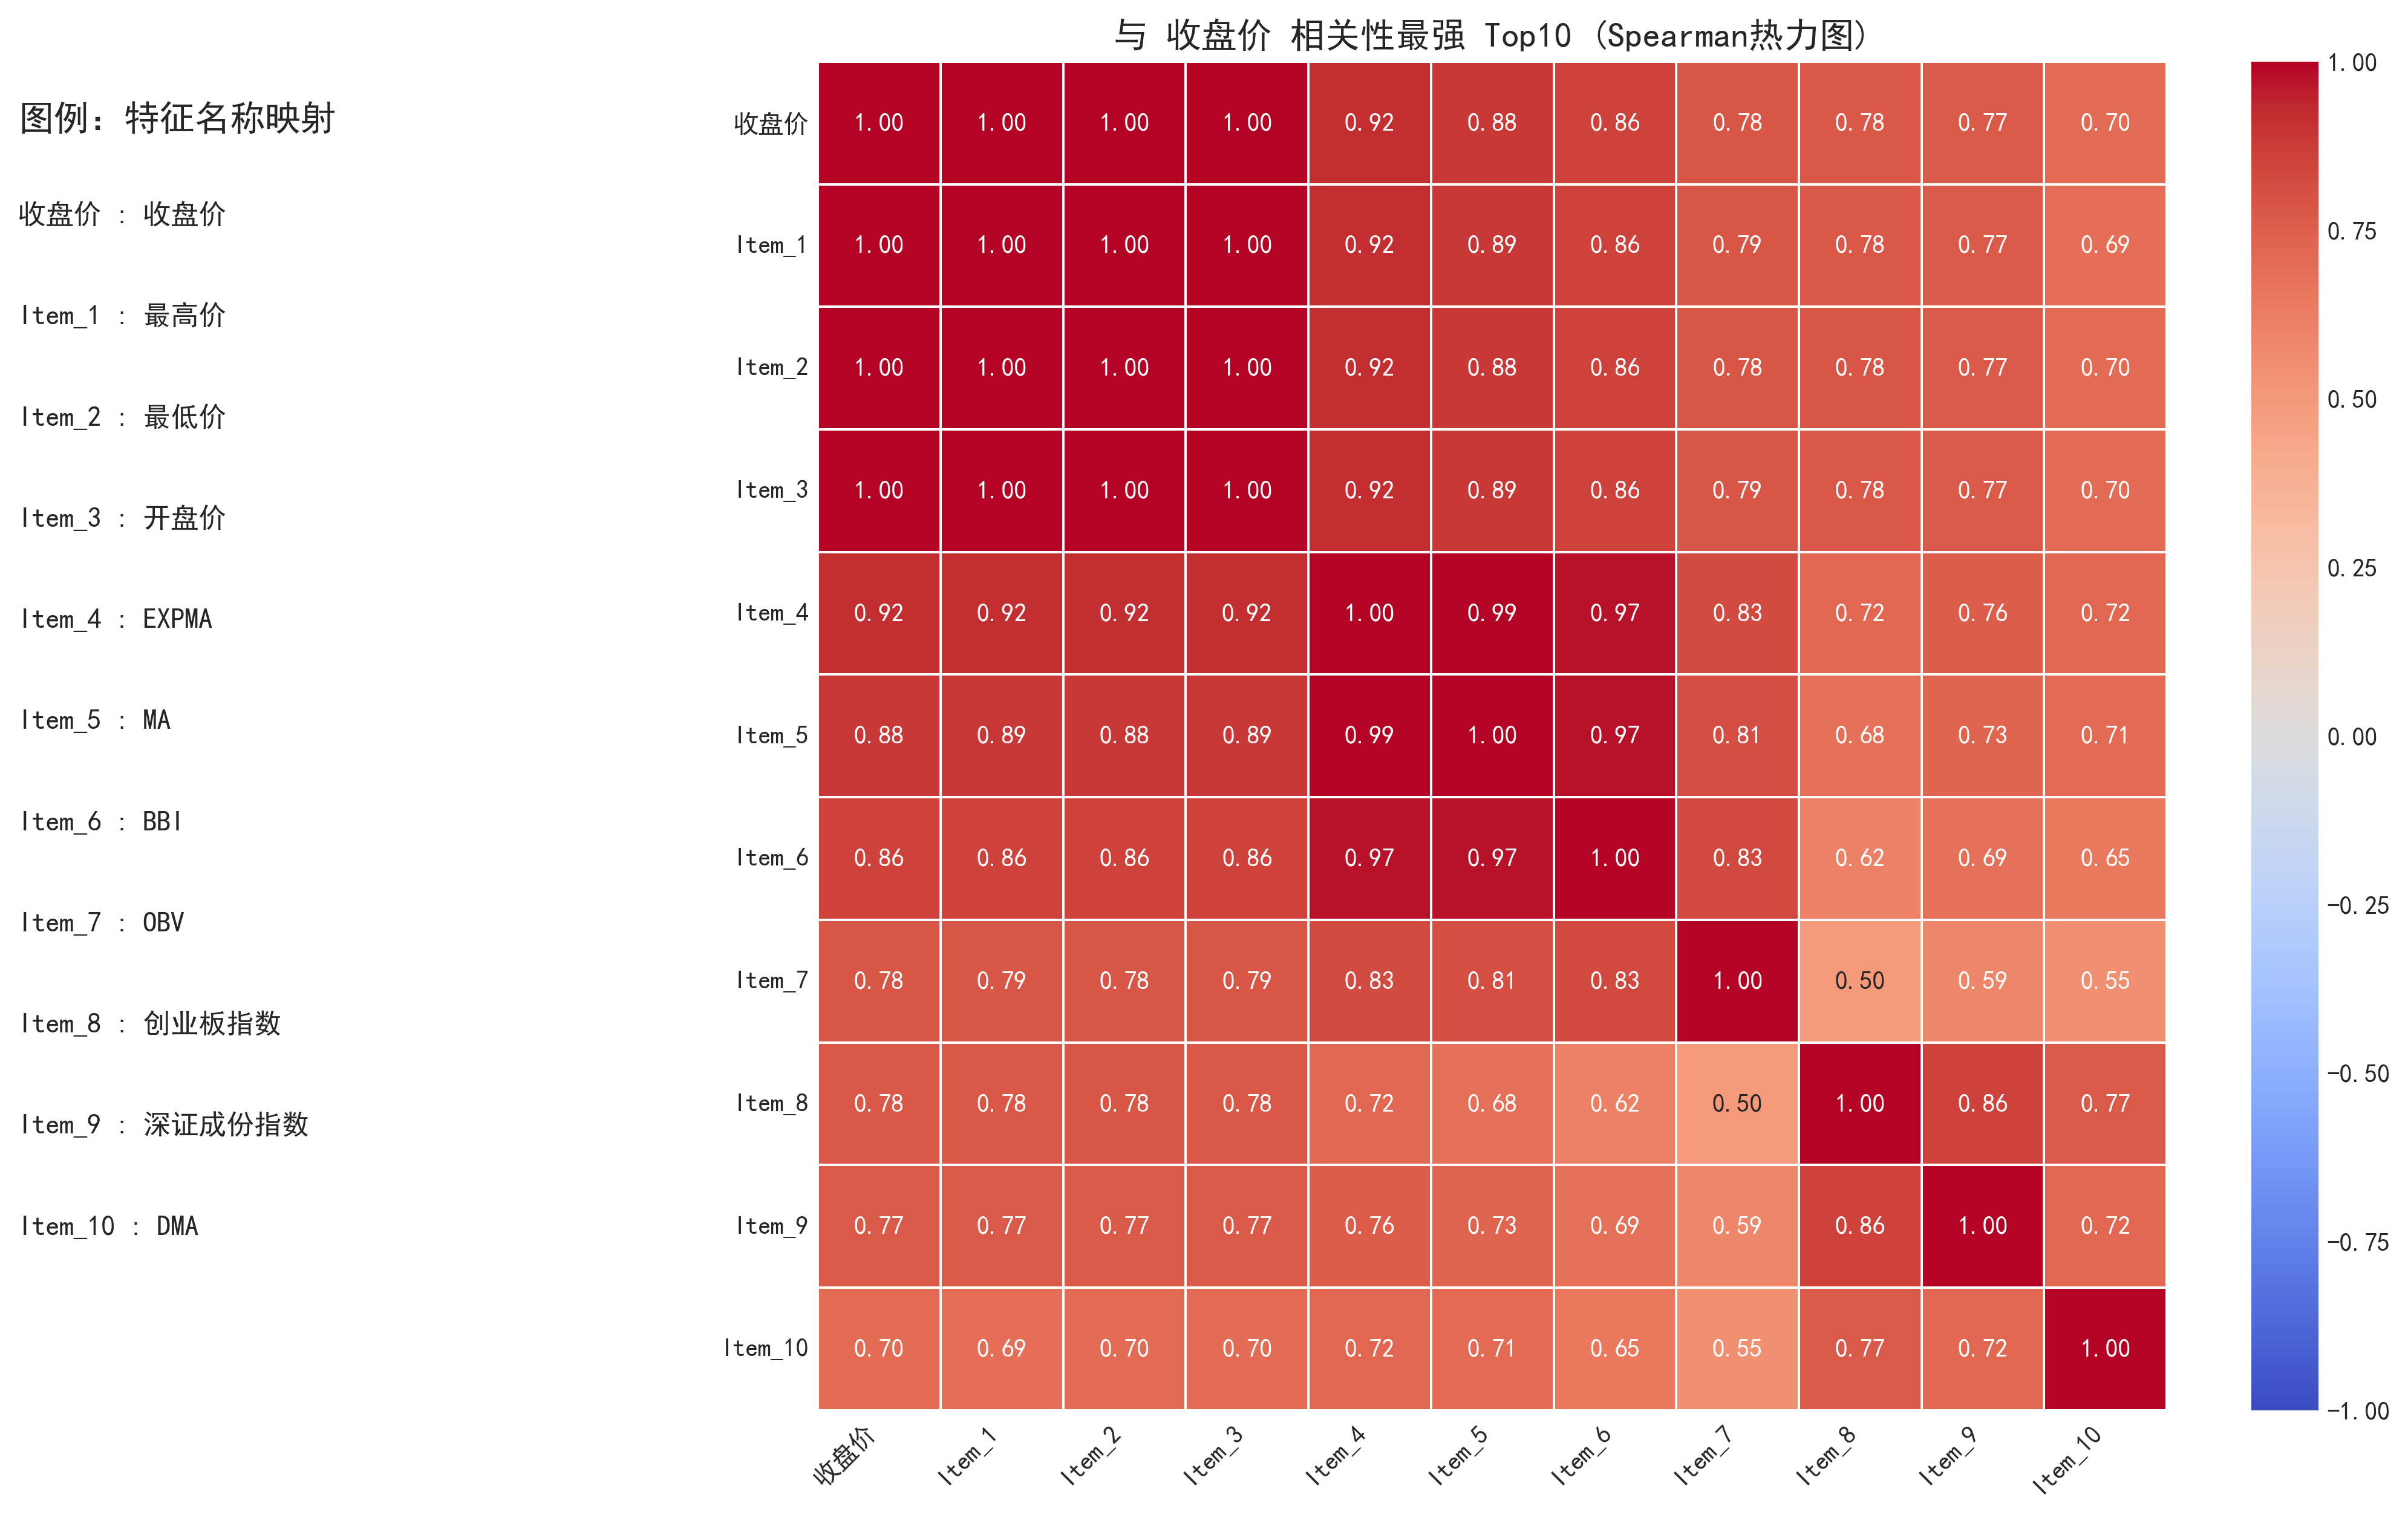
\includegraphics[width=0.88\textwidth]{figures/heatmap_收盘价.png}
    \caption{与收盘价相关性最强的Top10特征热力图（Spearman）}
    \label{fig:heatmap_price}
\end{figure}

由图~\ref{fig:heatmap_price} 可以看出，与收盘价相关性较强的特征主要集中在趋势动量与跨市场联动指标上，说明价格序列更容易受到方向性和外部市场传导的共同影响。

\begin{figure}[H]
    \centering
    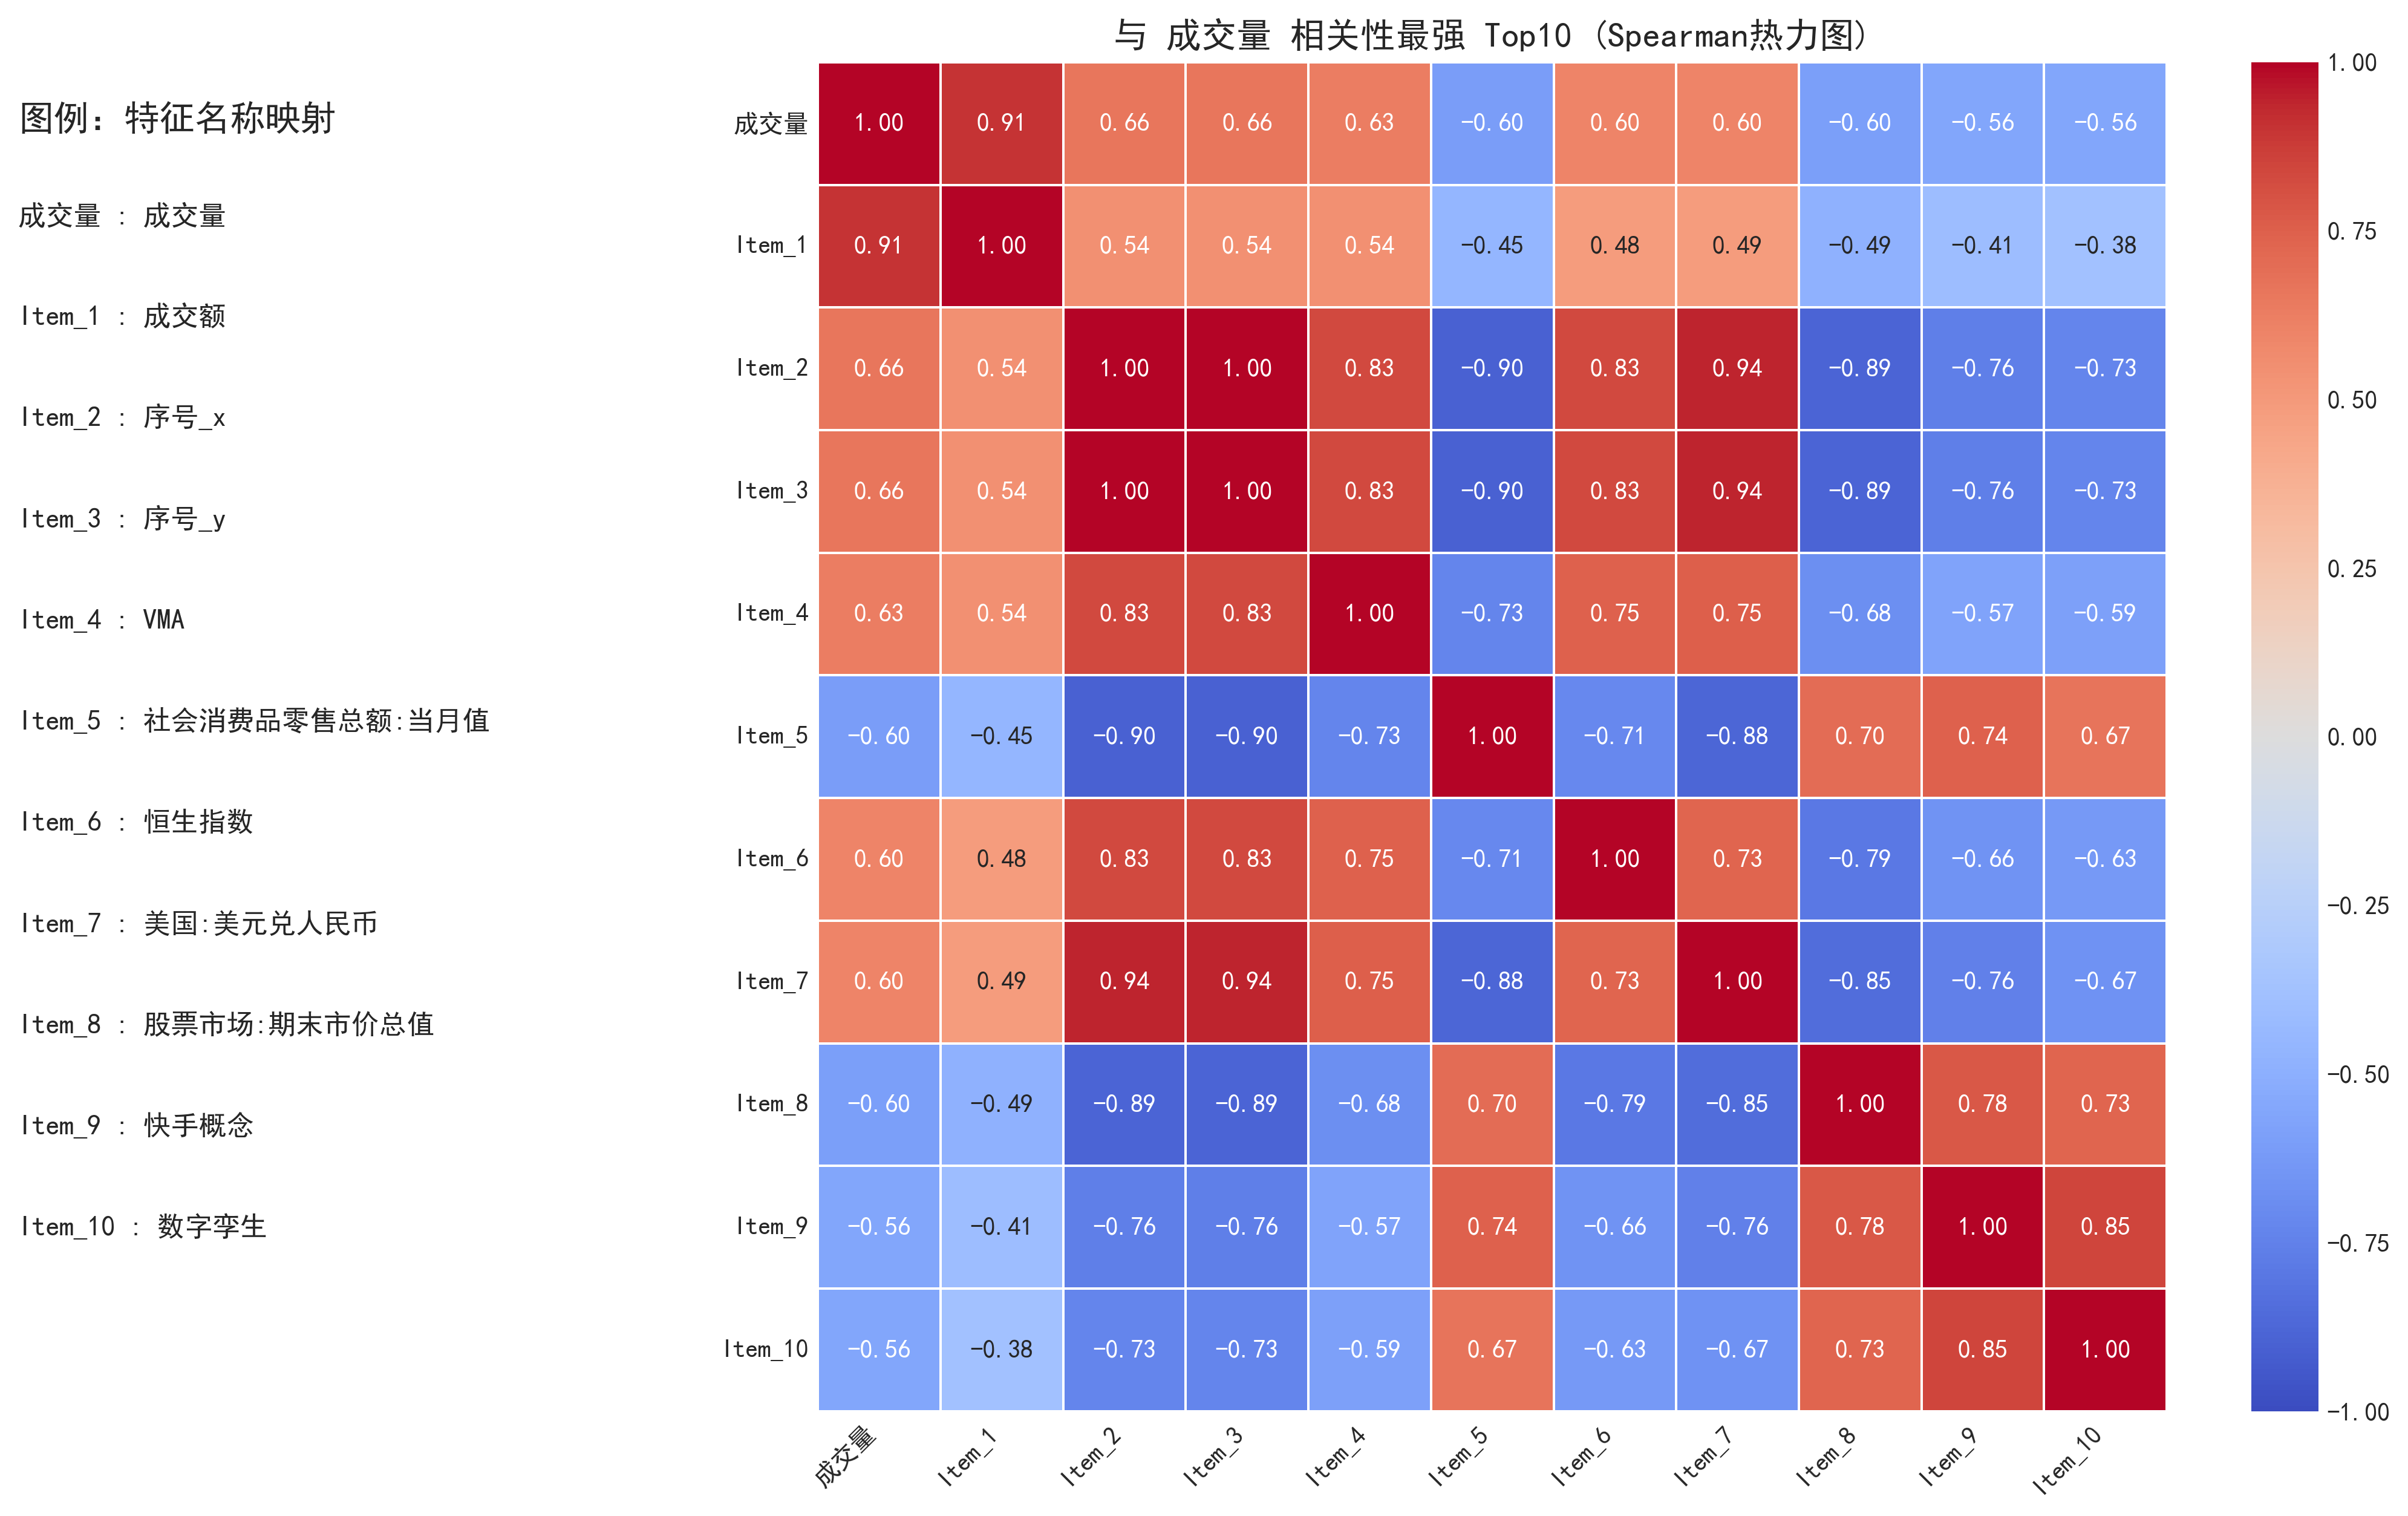
\includegraphics[width=0.88\textwidth]{figures/heatmap_成交量.png}
    \caption{与成交量相关性最强的Top10特征热力图（Spearman）}
    \label{fig:heatmap_volume}
\end{figure}

由图~\ref{fig:heatmap_volume} 可以看出，与成交量相关性较强的特征更多反映流动性变化与日内交易活跃度，表明成交量对资金流动和市场情绪的响应更直接。

\subsection{高频时间序列统计特性分析}

进一步分析发现，数字经济板块高频数据具有典型的金融时间序列统计特征。

\subsubsection{非平稳性}

高频金融价格会随着市场情绪、宏观政策以及板块轮动持续变化，因此其统计特征并不固定。

设时间序列为 $X_t$，若满足：

\begin{equation}
E(X_t)\neq C
\end{equation}

或：

\begin{equation}
Var(X_t)\neq C
\end{equation}

则说明序列不满足平稳性条件。

通过观察原始价格走势可以发现，其均值与波动水平均随时间变化，因此原始价格序列属于典型非平稳时间序列。

\subsubsection{波动聚集性}

金融市场中通常存在“波动聚集”现象，即：大波动之后仍倾向于出现大波动，小波动之后仍倾向于出现小波动。这一现象在高频市场中尤为明显。

\begin{figure}[H]
    \centering
    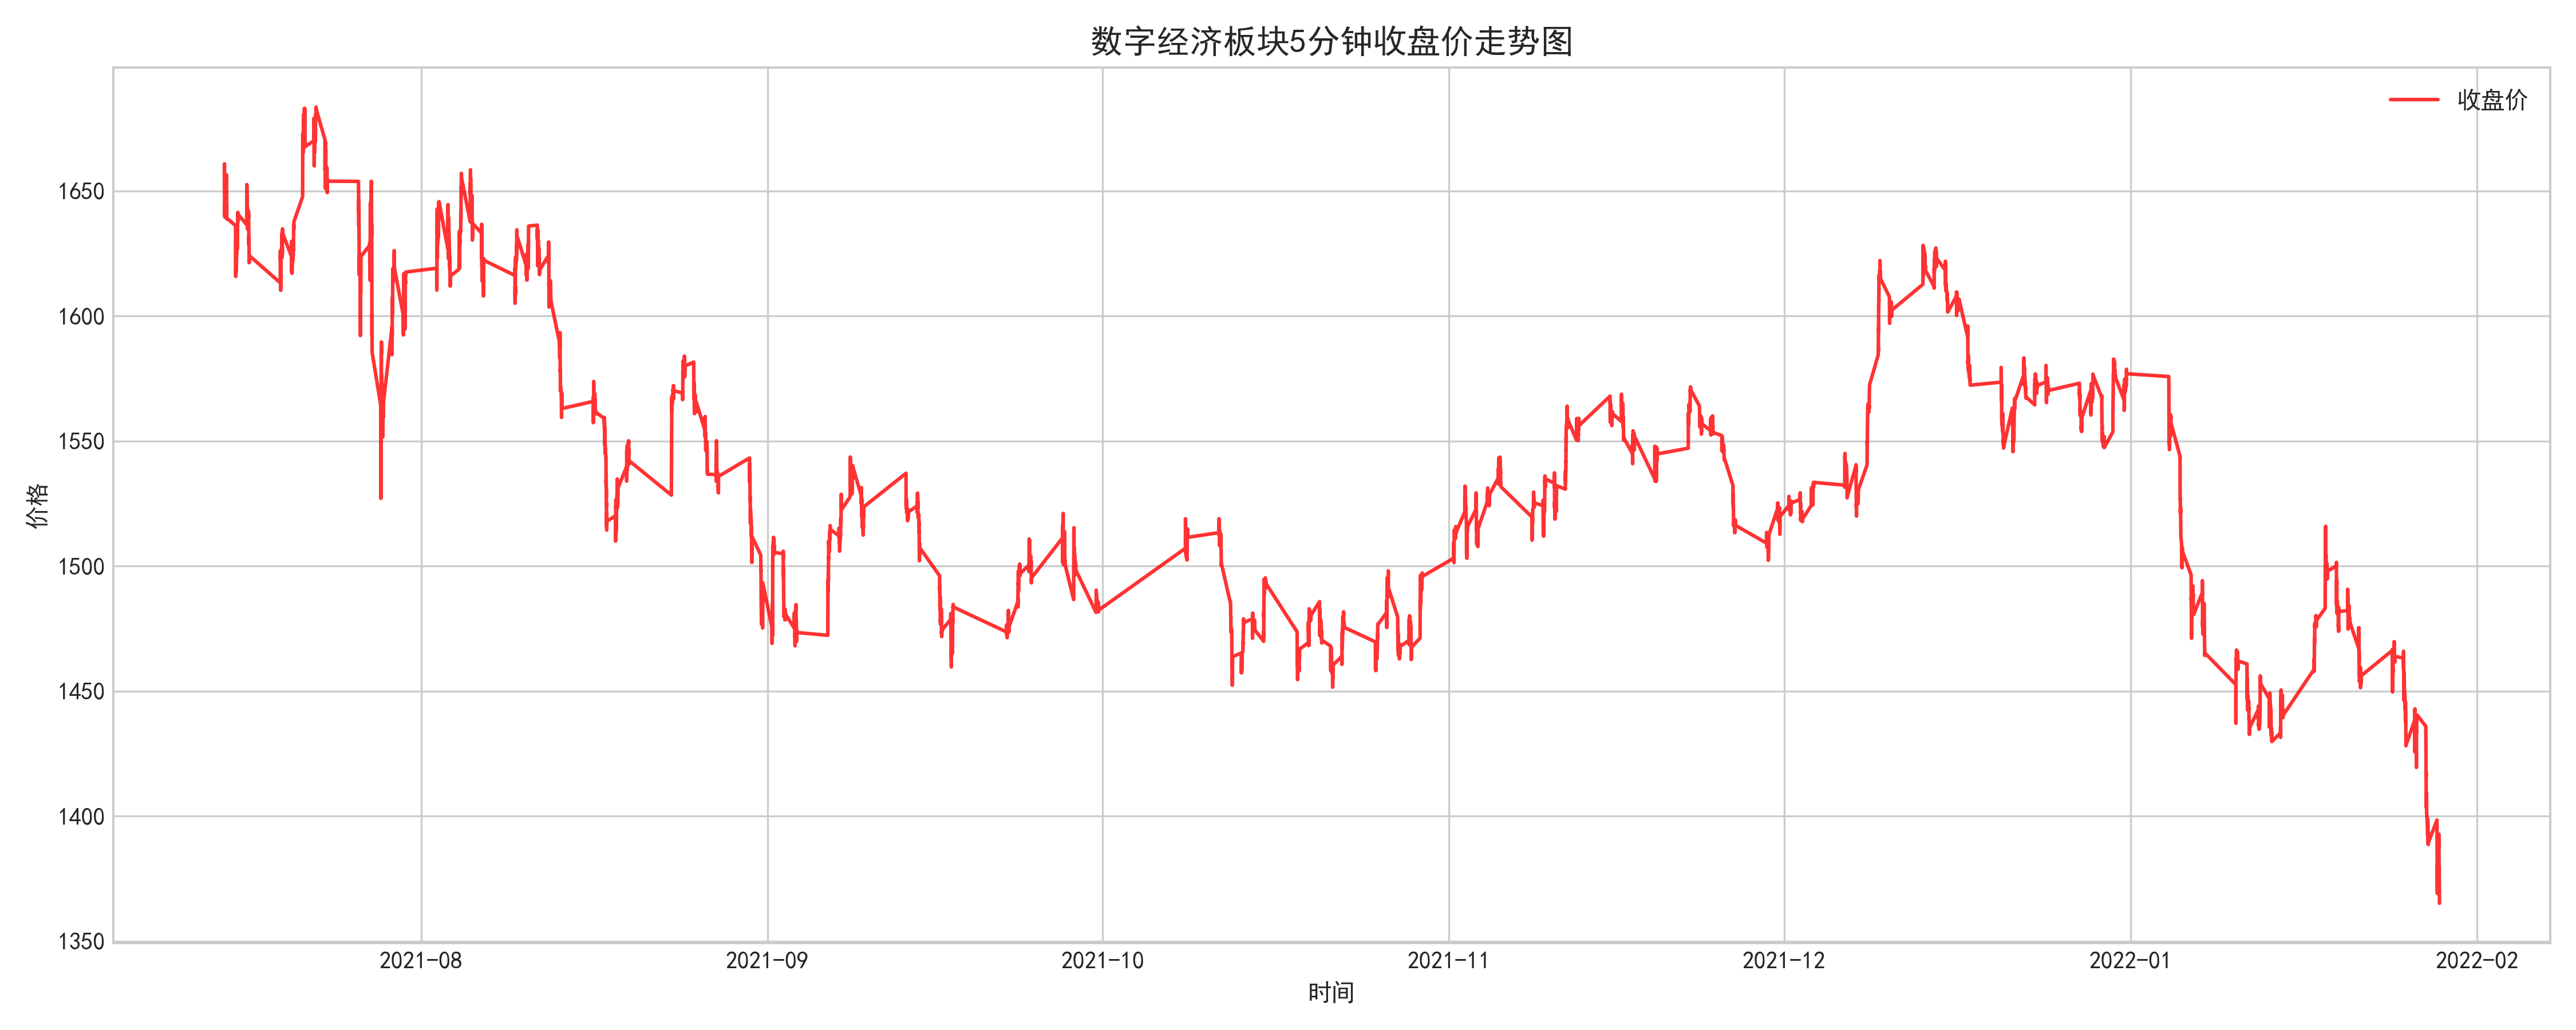
\includegraphics[width=0.9\textwidth]{figures/price_trend.png}
    \caption{数字经济板块收盘价时序走势}
    \label{fig:price_trend}
\end{figure}

由图~\ref{fig:price_trend} 可以看出，价格序列存在明显的局部趋势性与波动聚集特征。

\subsubsection{高频噪声特征}

相比日线数据，高频数据更容易受到：高频交易行为、短期情绪冲击、微观成交扰动、流动性瞬时变化等因素影响，因此其随机噪声显著增强。

这意味着模型不仅需要学习长期趋势，还需要具备较强的局部波动鲁棒性。

\subsection{成交量日内结构分析}

进一步分析成交量序列后发现，其在日内交易过程中具有明显的“U型结构”。

具体表现为：开盘阶段成交量迅速放大；午间阶段成交量明显下降；收盘阶段再次出现成交峰值。

这一现象主要来源于：开盘阶段信息集中释放；机构资金集中调仓；收盘集合竞价交易；日内短线资金平仓行为。

因此，成交量序列并非简单随机波动，而是具有明显的时间位置依赖特征。

\begin{figure}[H]
    \centering
    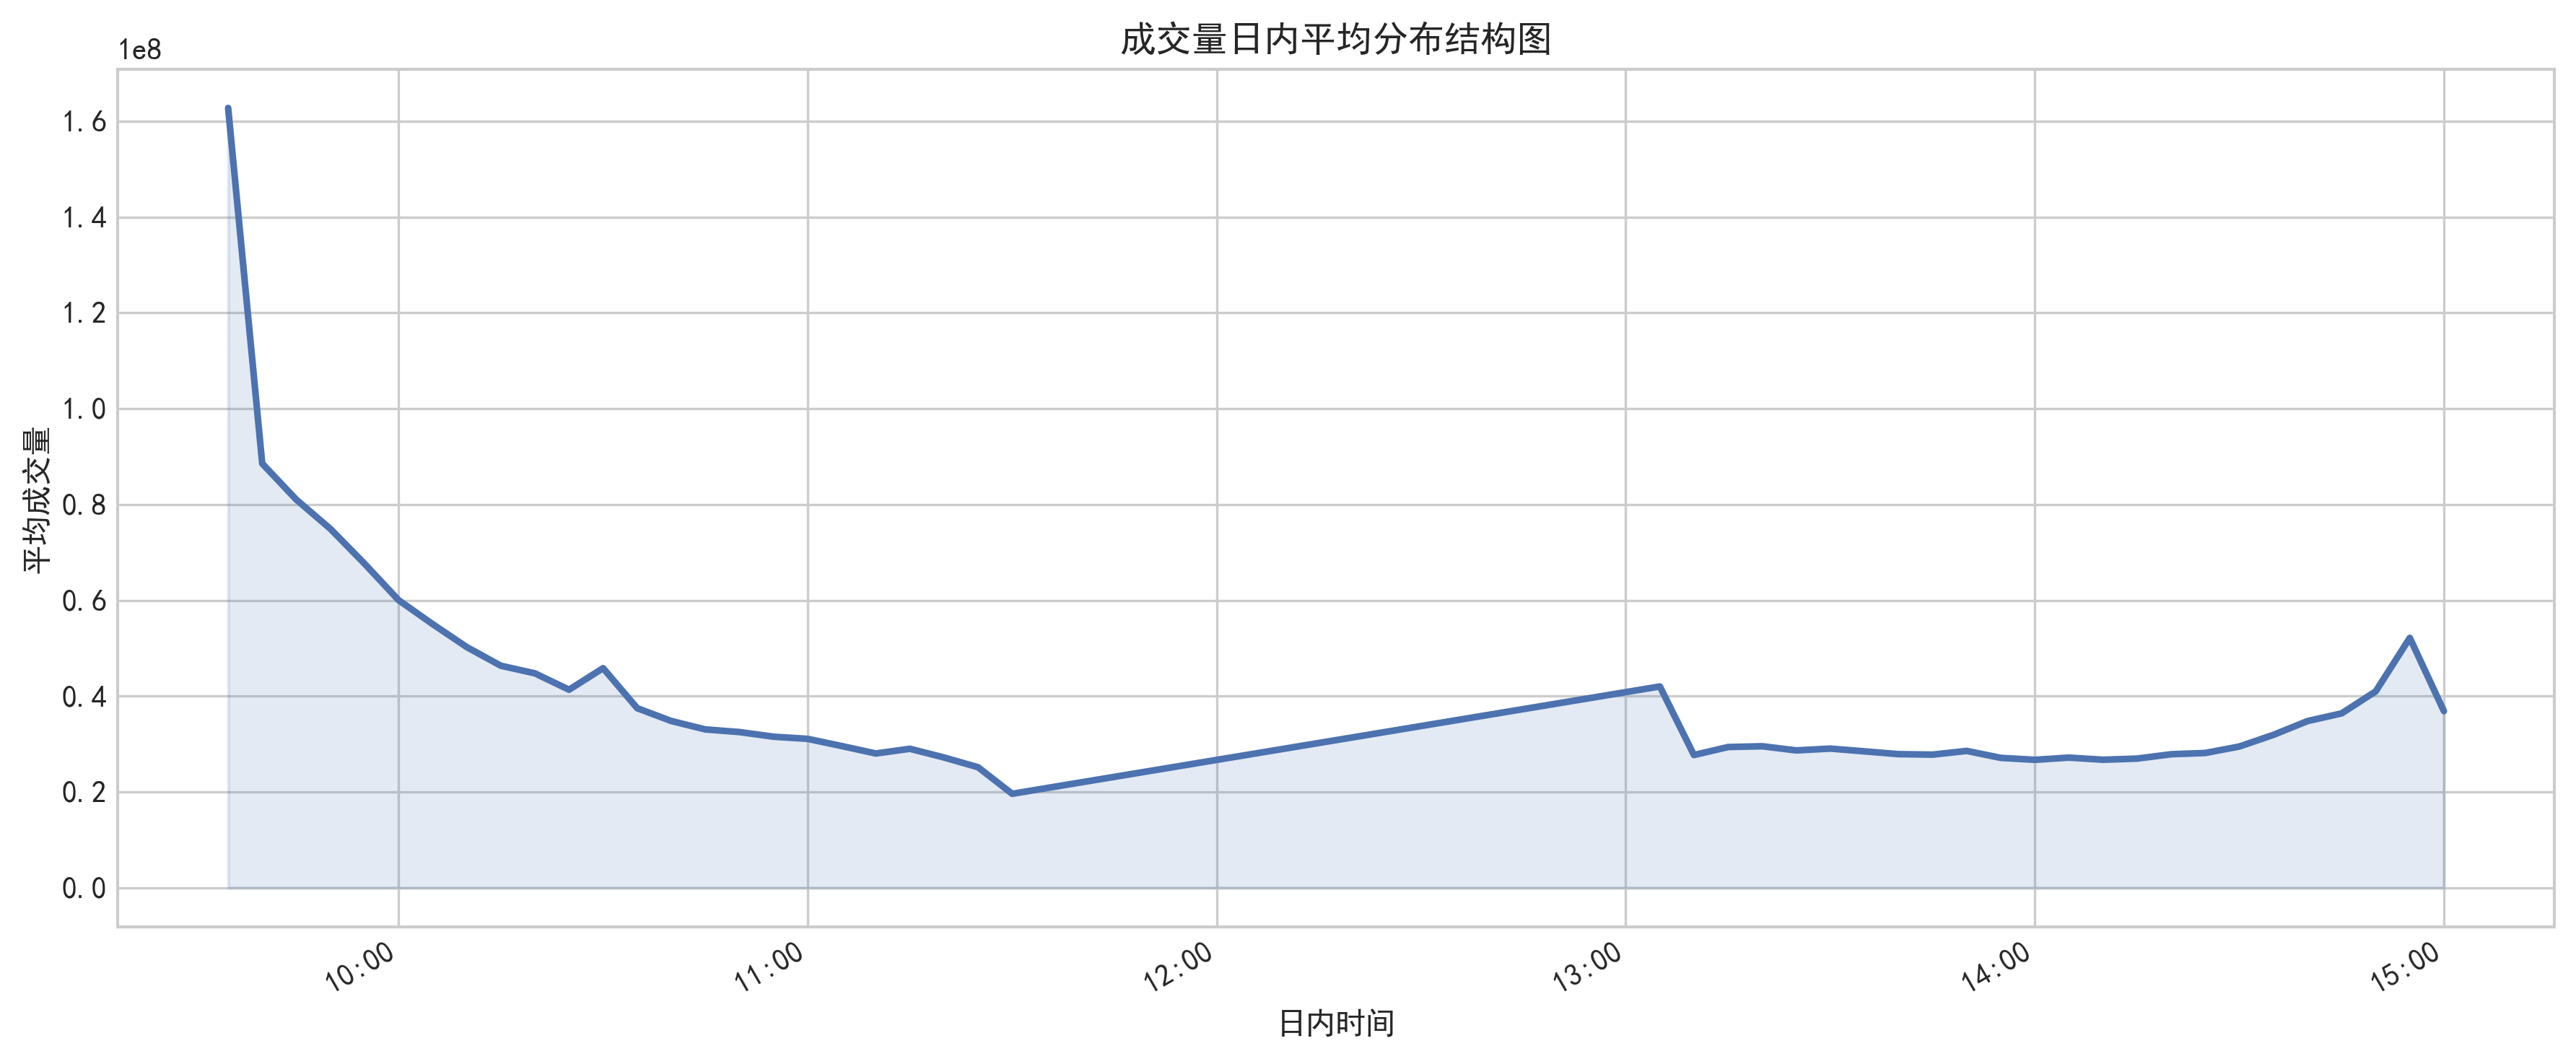
\includegraphics[width=0.88\textwidth]{figures/intraday_volume_pattern.png}
    \caption{成交量日内平均分布结构}
    \label{fig:intraday_volume}
\end{figure}

由图~\ref{fig:intraday_volume} 可以明显观察到，成交量在开盘与收盘阶段形成双峰结构，而中间交易时段整体较为平稳。

这一发现对于后续成交量预测模型具有重要意义。

在初始建模阶段，本文曾尝试采用与收盘价相同的方式直接预测成交量，但由于开盘阶段存在极端成交量峰值，模型训练过程被少量尖峰样本主导，最终导致整体预测基线发生严重漂移。

因此，在后续模型建立阶段，需要针对成交量序列的长尾分布与日内周期结构进行专门优化。

\subsection{本节小结}

本节首先对数字经济板块高频数据进行了系统的数据预处理与探索性分析，完成了：缺失值修补；时间对齐；异常值平滑；高频统计特性分析；日内成交结构分析。

分析结果表明：收盘价整体具有局部趋势性与波动聚集特征；成交量具有明显长尾分布与日内U型结构；高频金融数据存在显著非平稳性与异方差特征；传统统一建模方法难以同时适配价格与成交量序列。

因此，在后续模型建立过程中，需要针对不同金融变量的统计特性分别设计预测策略，以提高模型稳定性与预测精度。

%% ============================================================================
\section{特征分析与指标提取}

高频金融市场具有典型的非线性、非平稳以及强随机波动特征，仅依赖原始价格序列难以充分刻画市场运行规律。因此，在模型建立之前，需要进一步构建能够反映趋势、波动、动量以及市场情绪的金融特征指标。

合理的特征工程不仅能够增强模型对市场状态的表达能力，还能够有效提升预测稳定性与交易策略鲁棒性。

本文结合高频量化交易特点，从以下几个层面构建特征体系：基础价格特征；收益率与波动率特征；技术指标特征；成交量结构特征；时间周期特征；跨市场关联特征。

最终形成面向高频预测任务的多维金融特征矩阵。

\subsection{基础价格特征构建}

价格信息是金融市场最核心的数据来源。

本文首先基于原始K线数据提取基础价格特征，包括：开盘价（Open）、收盘价（Close）、最高价（High）、最低价（Low）、振幅（Amplitude）、涨跌幅（Return）。

其中，振幅定义为：

\begin{equation}
A_t=\frac{High_t-Low_t}{Close_t}
\end{equation}

涨跌幅定义为：

\begin{equation}
R_t=\frac{Close_t-Close_{t-1}}{Close_{t-1}}
\end{equation}

相比直接使用价格绝对值，收益率序列能够有效削弱长期趋势影响，使模型更关注局部价格变化。

此外，收益率还能够提高不同时间阶段之间的数据可比性。

\begin{figure}[H]
    \centering
    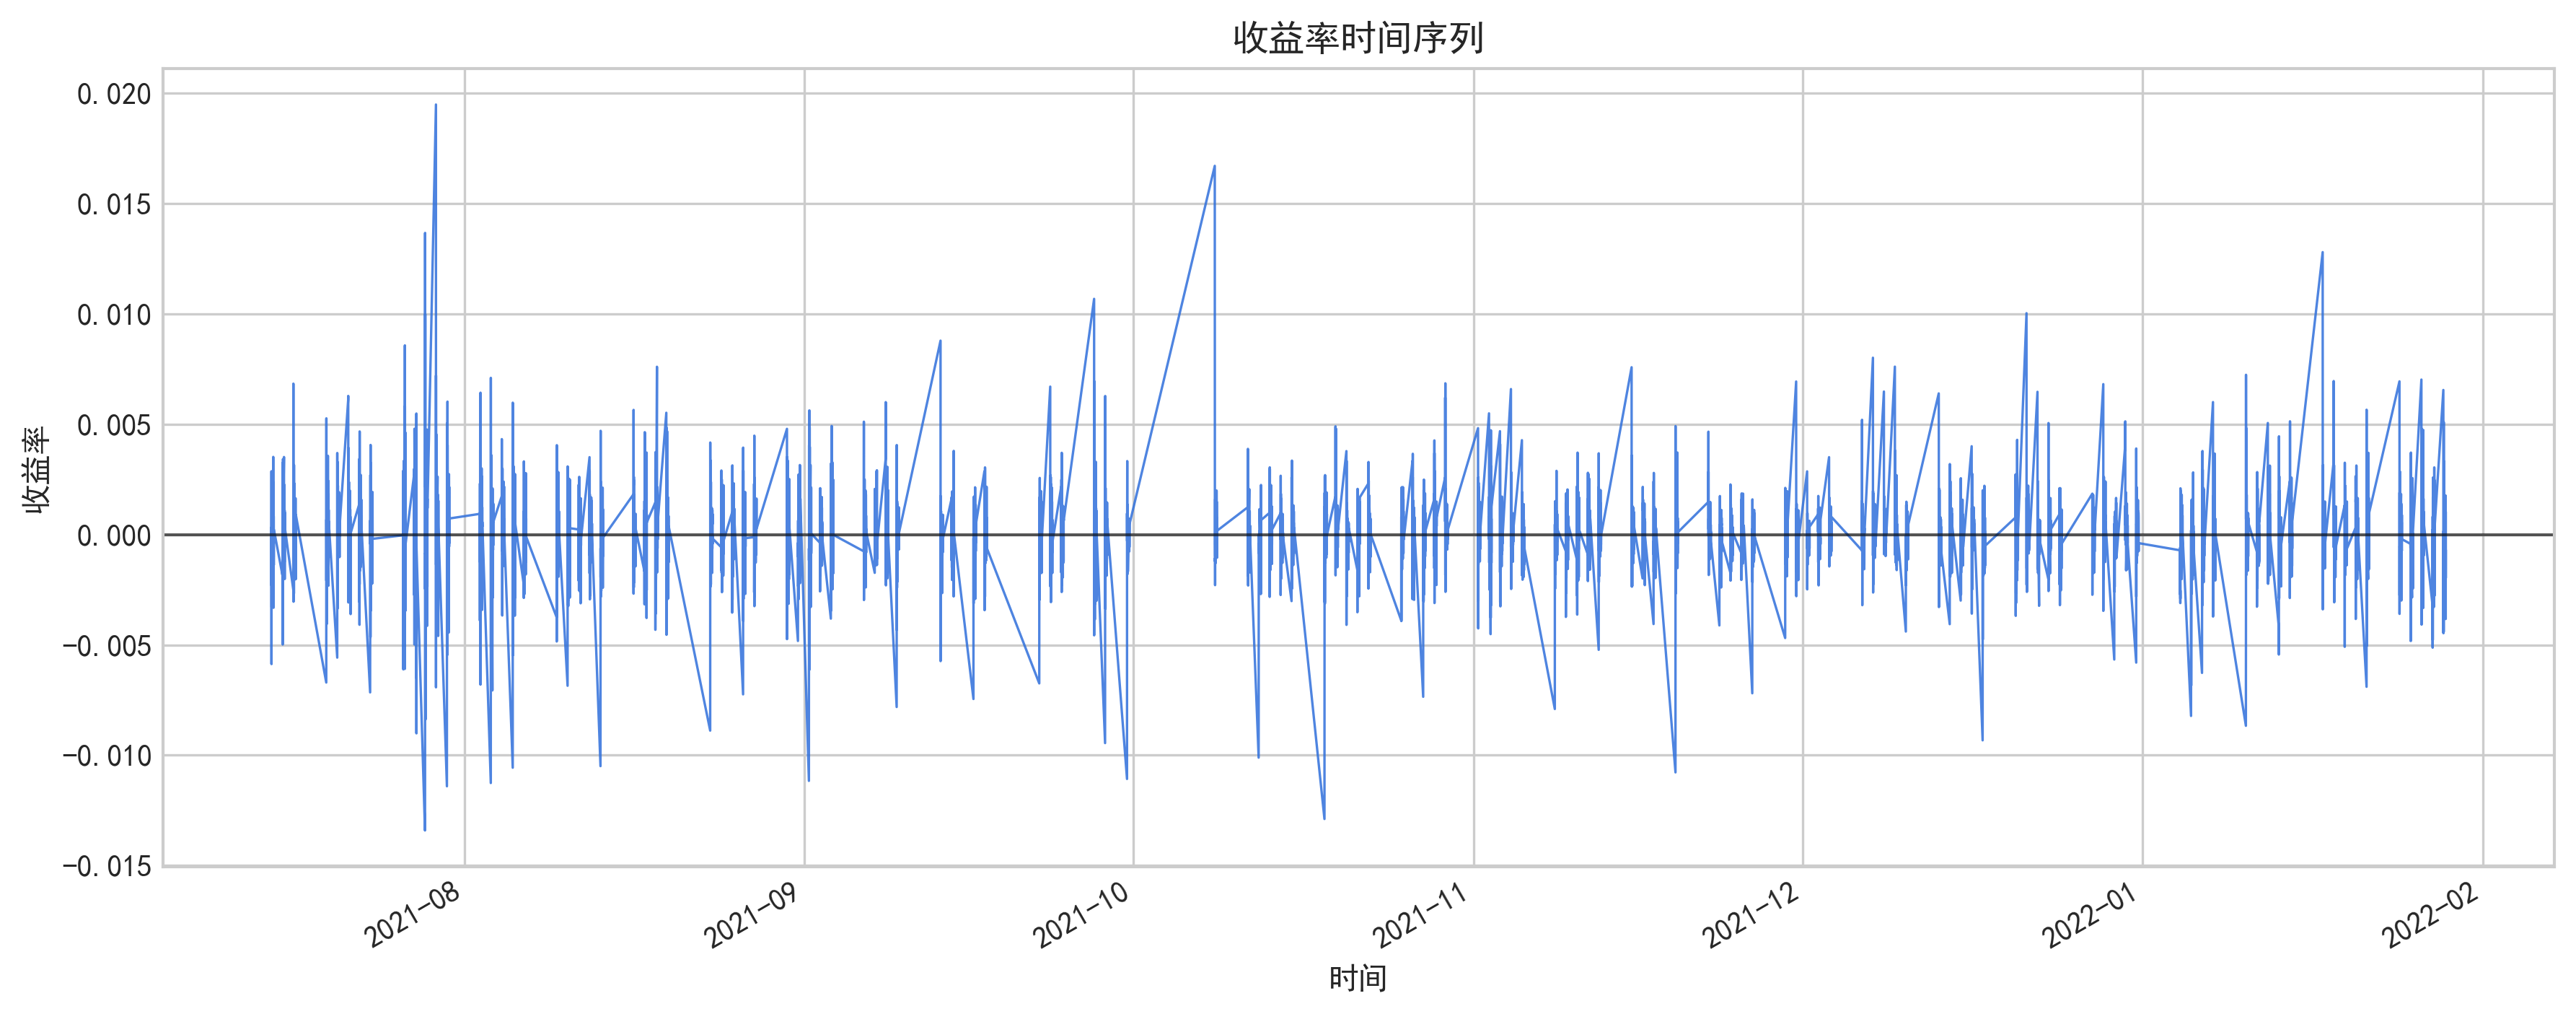
\includegraphics[width=0.9\textwidth]{figures/return_series.png}
    \caption{收益率时间序列}
    \label{fig:return_series}
\end{figure}

由图~\ref{fig:return_series} 可以看出，高频收益率整体围绕零值上下波动，具有明显的短期随机扰动特征。

\subsection{移动平均趋势特征}

金融市场中存在典型的趋势惯性现象，因此本文进一步引入移动平均（Moving Average, MA）特征。

设窗口长度为 $n$，则移动平均定义为：

\begin{equation}
MA_n(t)=\frac{1}{n}\sum_{i=0}^{n-1}Close_{t-i}
\end{equation}

本文分别构建：MA5、MA10、MA20、MA60。

不同时间尺度的移动平均能够反映市场短期、中期以及长期趋势结构。

其中：短周期均线对局部波动更敏感；长周期均线能够反映整体趋势方向。

同时，均线之间的相对位置还能够反映市场趋势强弱。

例如：

\begin{equation}
MA5 > MA20
\end{equation}

通常意味着市场处于短期上升趋势。

\begin{figure}[H]
    \centering
    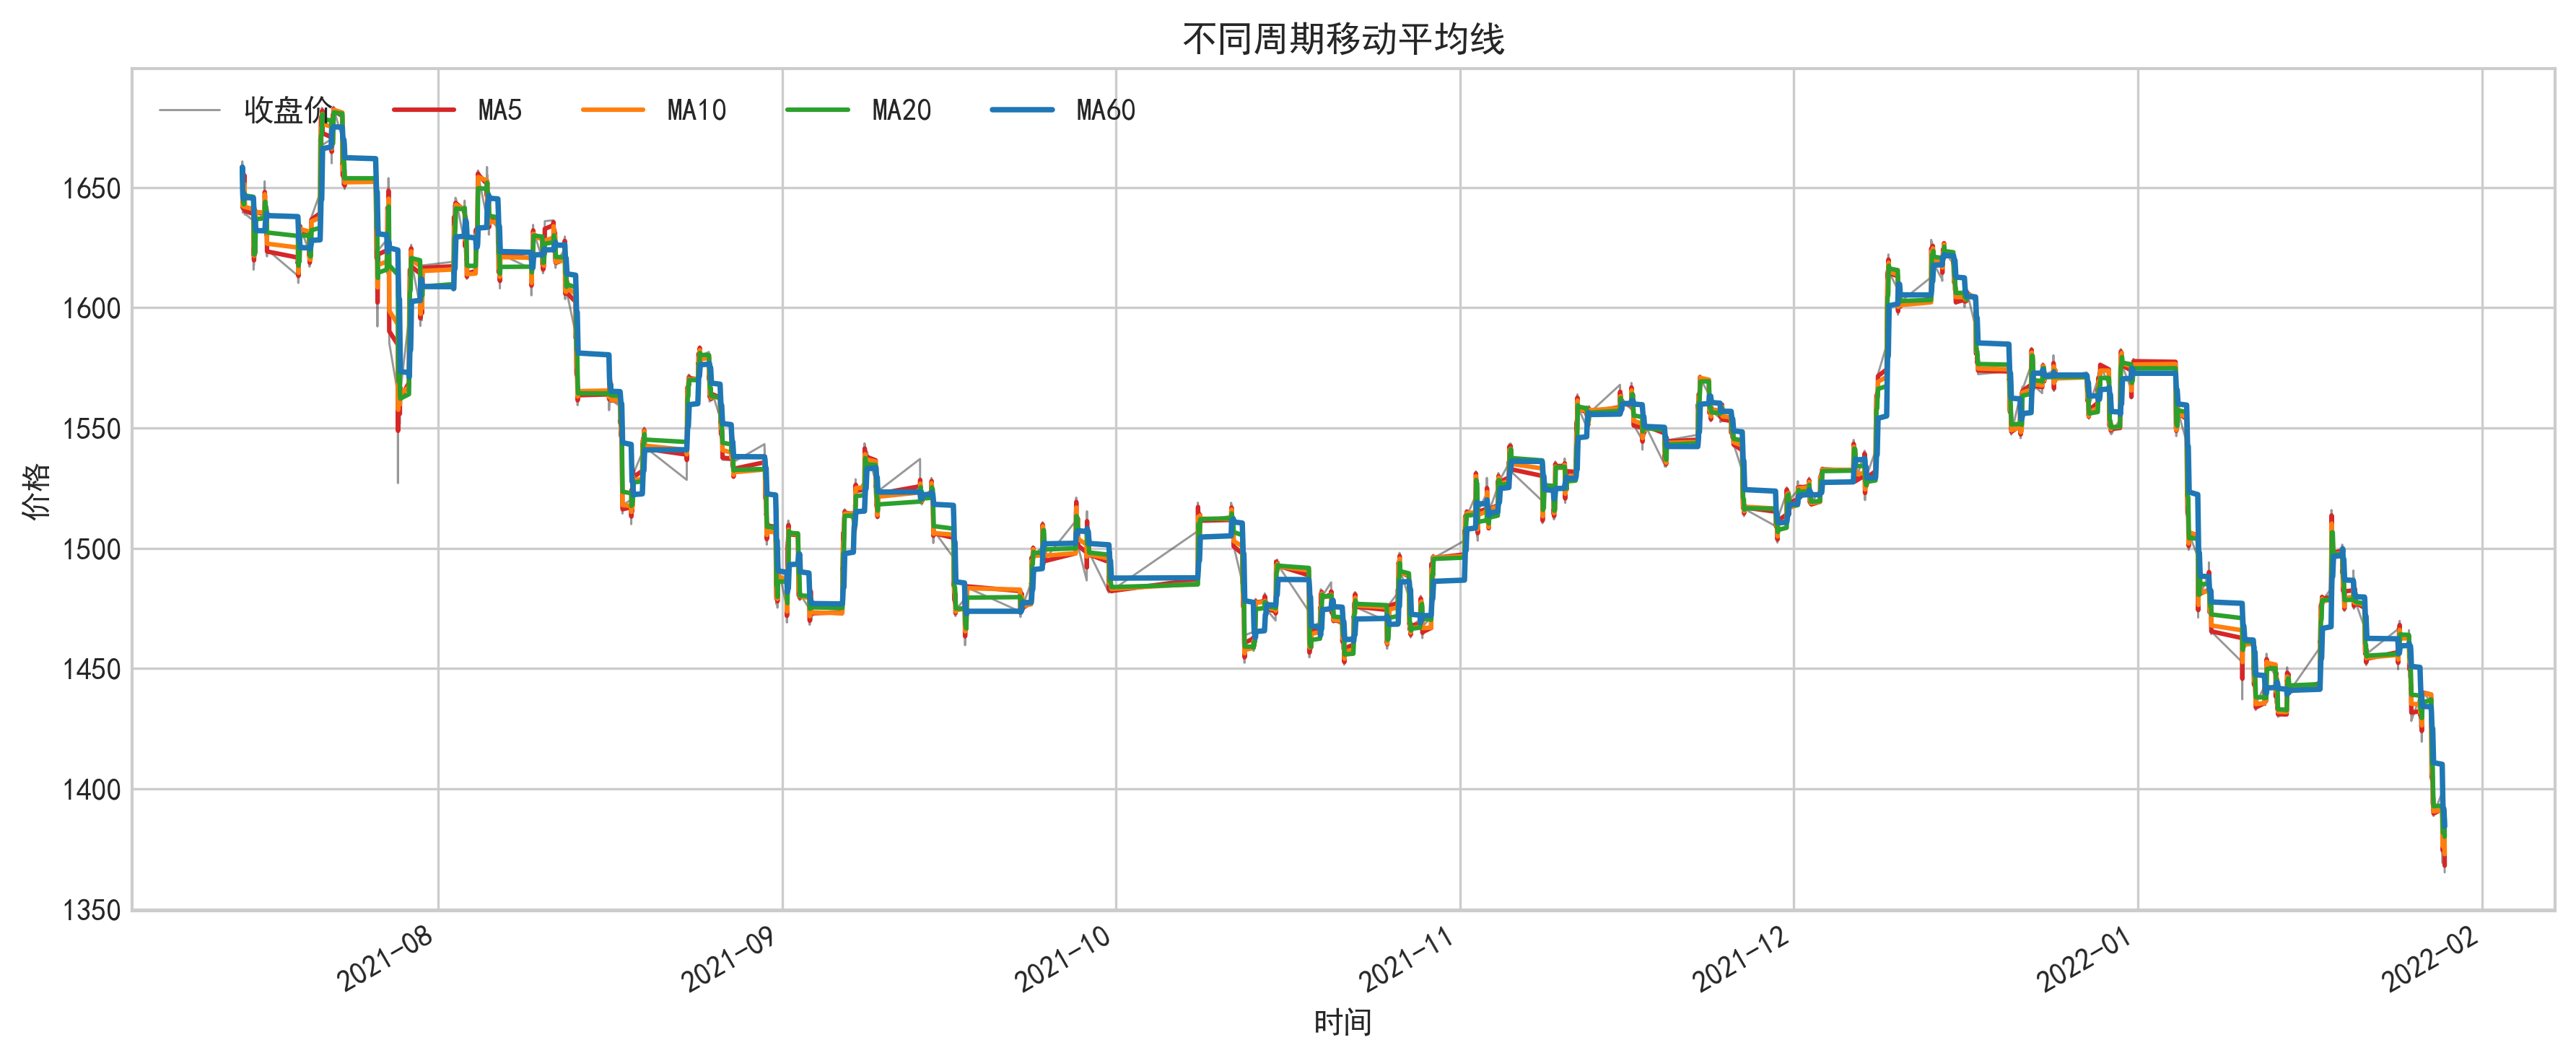
\includegraphics[width=0.92\textwidth]{figures/ma_compare.png}
    \caption{不同周期移动平均线}
    \label{fig:ma_compare}
\end{figure}

由图~\ref{fig:ma_compare} 可以看出，短周期均线波动更加灵敏，而长周期均线整体更加平滑。

\subsection{波动率特征构建}

高频金融市场中，波动率往往比价格本身更具有预测意义。

因此本文进一步构建局部波动率指标。

设窗口长度为 $n$，则滚动波动率定义为：

\begin{equation}
\sigma_t=\sqrt{\frac{1}{n}\sum_{i=0}^{n-1}(R_{t-i}-\bar{R})^2}
\end{equation}

其中：

\begin{equation}
\bar{R}=\frac{1}{n}\sum_{i=0}^{n-1}R_{t-i}
\end{equation}

波动率能够反映市场风险水平与情绪变化。

通常情况下：波动率快速上升意味着市场情绪剧烈变化；波动率下降则意味着市场进入平稳阶段。

\begin{figure}[H]
    \centering
    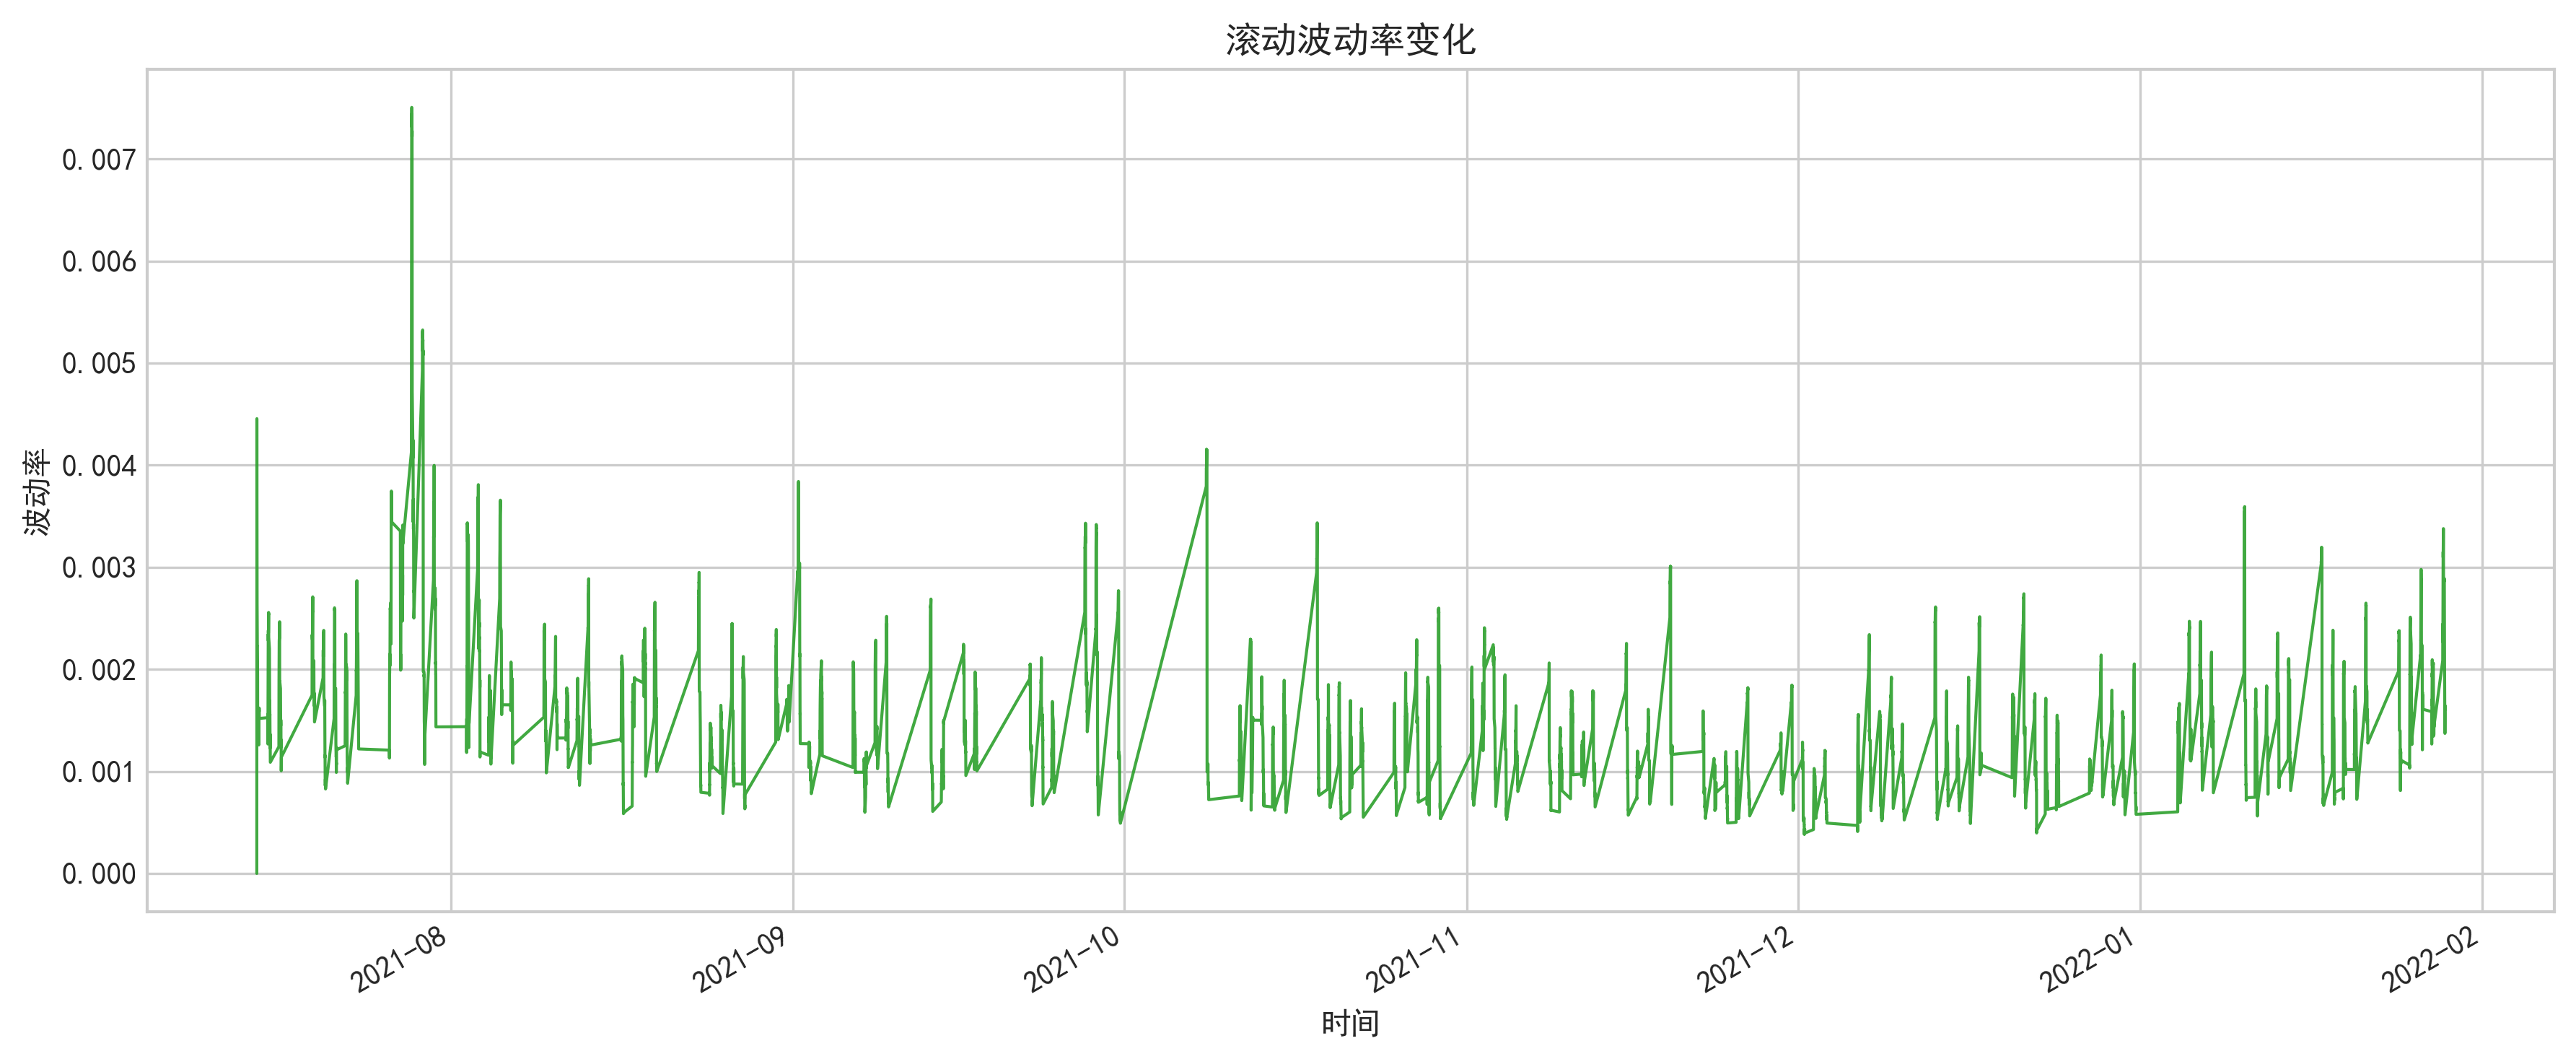
\includegraphics[width=0.88\textwidth]{figures/volatility_series.png}
    \caption{滚动波动率变化}
    \label{fig:volatility_series}
\end{figure}

由图~\ref{fig:volatility_series} 可以看出，市场波动率具有明显的聚集现象，即：

\begin{quote}
高波动之后仍容易出现高波动。
\end{quote}

这一结论与经典金融时间序列理论一致。

\subsection{MACD动量指标构建}

为了进一步增强模型对趋势变化的识别能力，本文引入 MACD（Moving Average Convergence Divergence）指标。

首先定义快慢指数移动平均：

\begin{equation}
EMA_{fast}=EMA(Close,12)
\end{equation}

\begin{equation}
EMA_{slow}=EMA(Close,26)
\end{equation}

则：

\begin{equation}
DIF=EMA_{fast}-EMA_{slow}
\end{equation}

进一步构建信号线：

\begin{equation}
DEA=EMA(DIF,9)
\end{equation}

最终得到 MACD 柱状图：

\begin{equation}
MACD=2(DIF-DEA)
\end{equation}

MACD 能够有效反映市场趋势方向与动量变化。

其中：MACD 上穿零轴通常意味着趋势转强，下穿零轴通常意味着趋势转弱。

\begin{figure}[H]
    \centering
    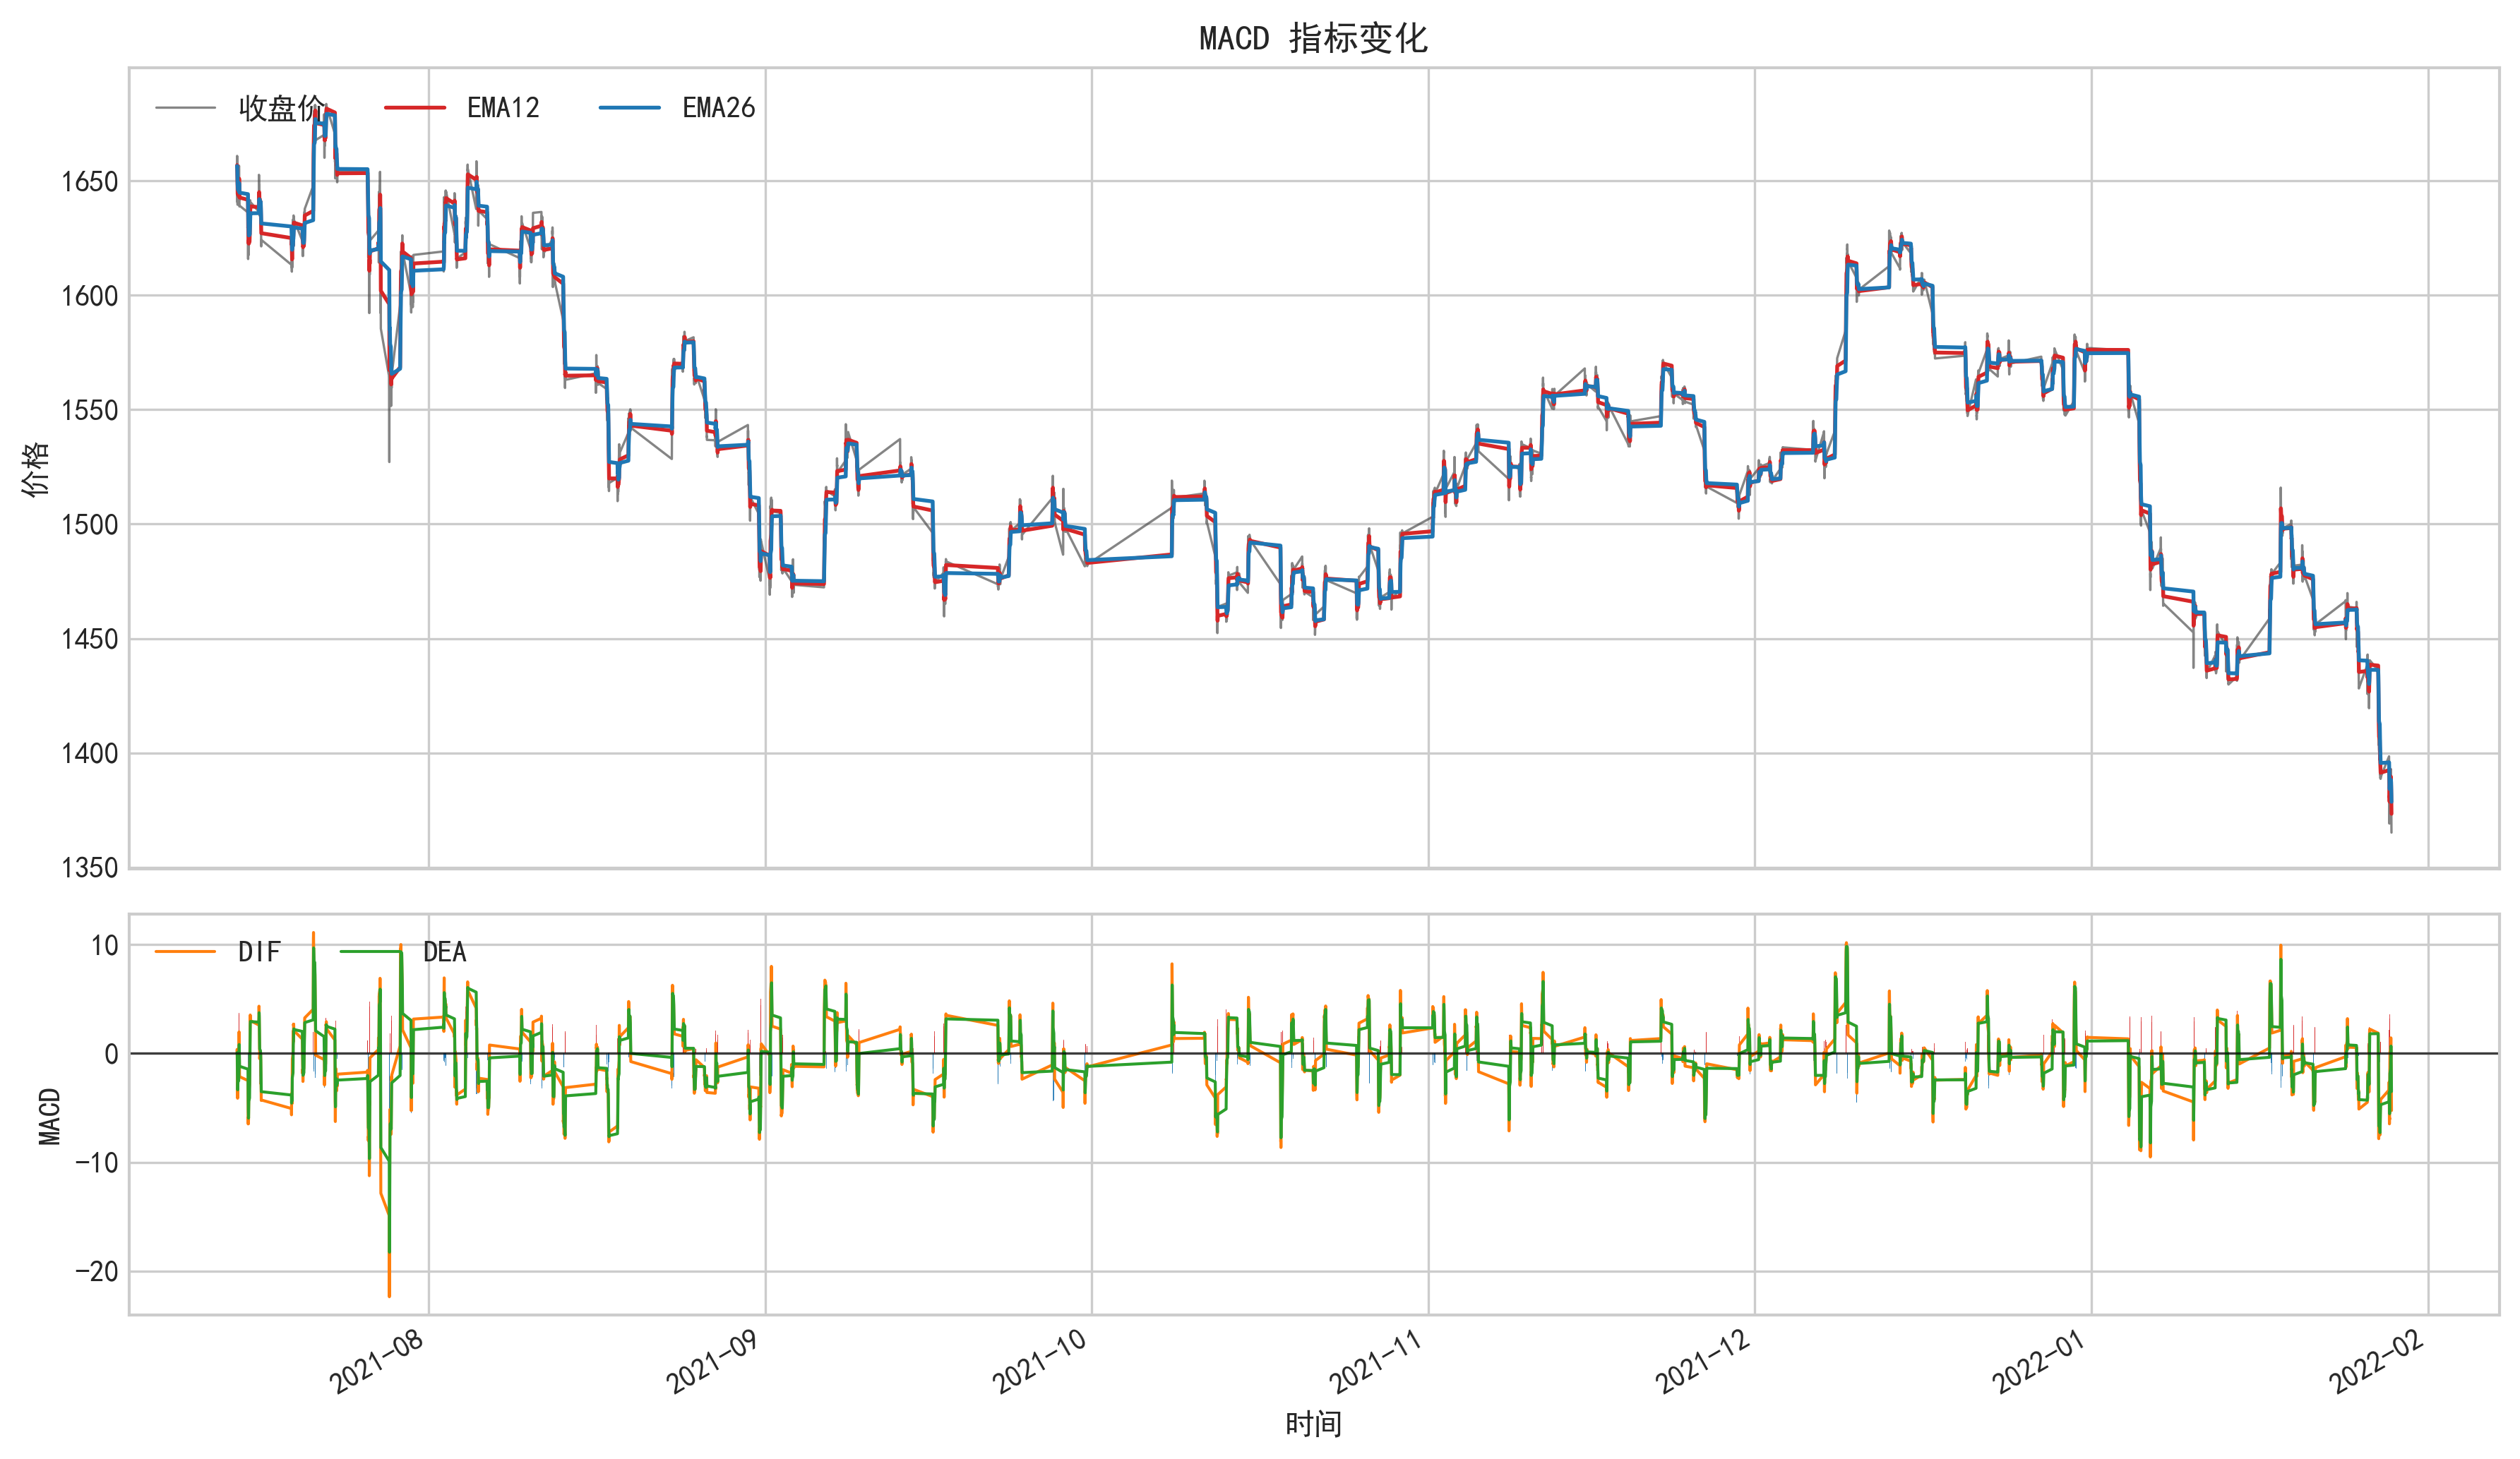
\includegraphics[width=0.9\textwidth]{figures/macd.png}
    \caption{MACD 指标变化}
    \label{fig:macd}
\end{figure}

\subsection{RSI超买超卖指标}

为了进一步识别市场短期情绪变化，本文构建 RSI（Relative Strength Index）指标。

设窗口长度为 $n$，则：

\begin{equation}
RS=\frac{Average\ Gain}{Average\ Loss}
\end{equation}

进一步定义：

\begin{equation}
RSI=100-\frac{100}{1+RS}
\end{equation}

RSI 能够反映市场买卖力量对比。

通常情况下：RSI > 70 表示市场可能进入超买区，RSI < 30 表示市场可能进入超卖区。

该指标能够帮助模型识别局部反转机会。

\subsection{成交量特征分析与建模差异}

成交量是高频金融市场中最重要的流动性指标之一。

然而，与收盘价相比，成交量具有完全不同的统计结构。

通过前文探索性分析已经发现：收盘价整体趋势较平滑；成交量则存在明显长尾尖峰结构；开盘与收盘阶段会出现集中放量现象。

因此，若直接采用与价格相同的建模方式处理成交量，容易导致模型训练被少量极端样本主导。

在初始实验阶段，本文曾尝试直接对原始成交量进行预测，但实验结果表明：模型整体预测基线明显上移；正常成交区间出现严重悬浮；局部波动趋势无法正确拟合；模型训练过程极不稳定。

其根本原因在于：成交量具有显著的右偏长尾分布与时段异方差结构，而传统均方误差会对开盘阶段的大成交量尖峰进行平方放大。

因此，模型会优先拟合少量极端峰值，而忽略大部分正常区间。

\begin{figure}[H]
    \centering
    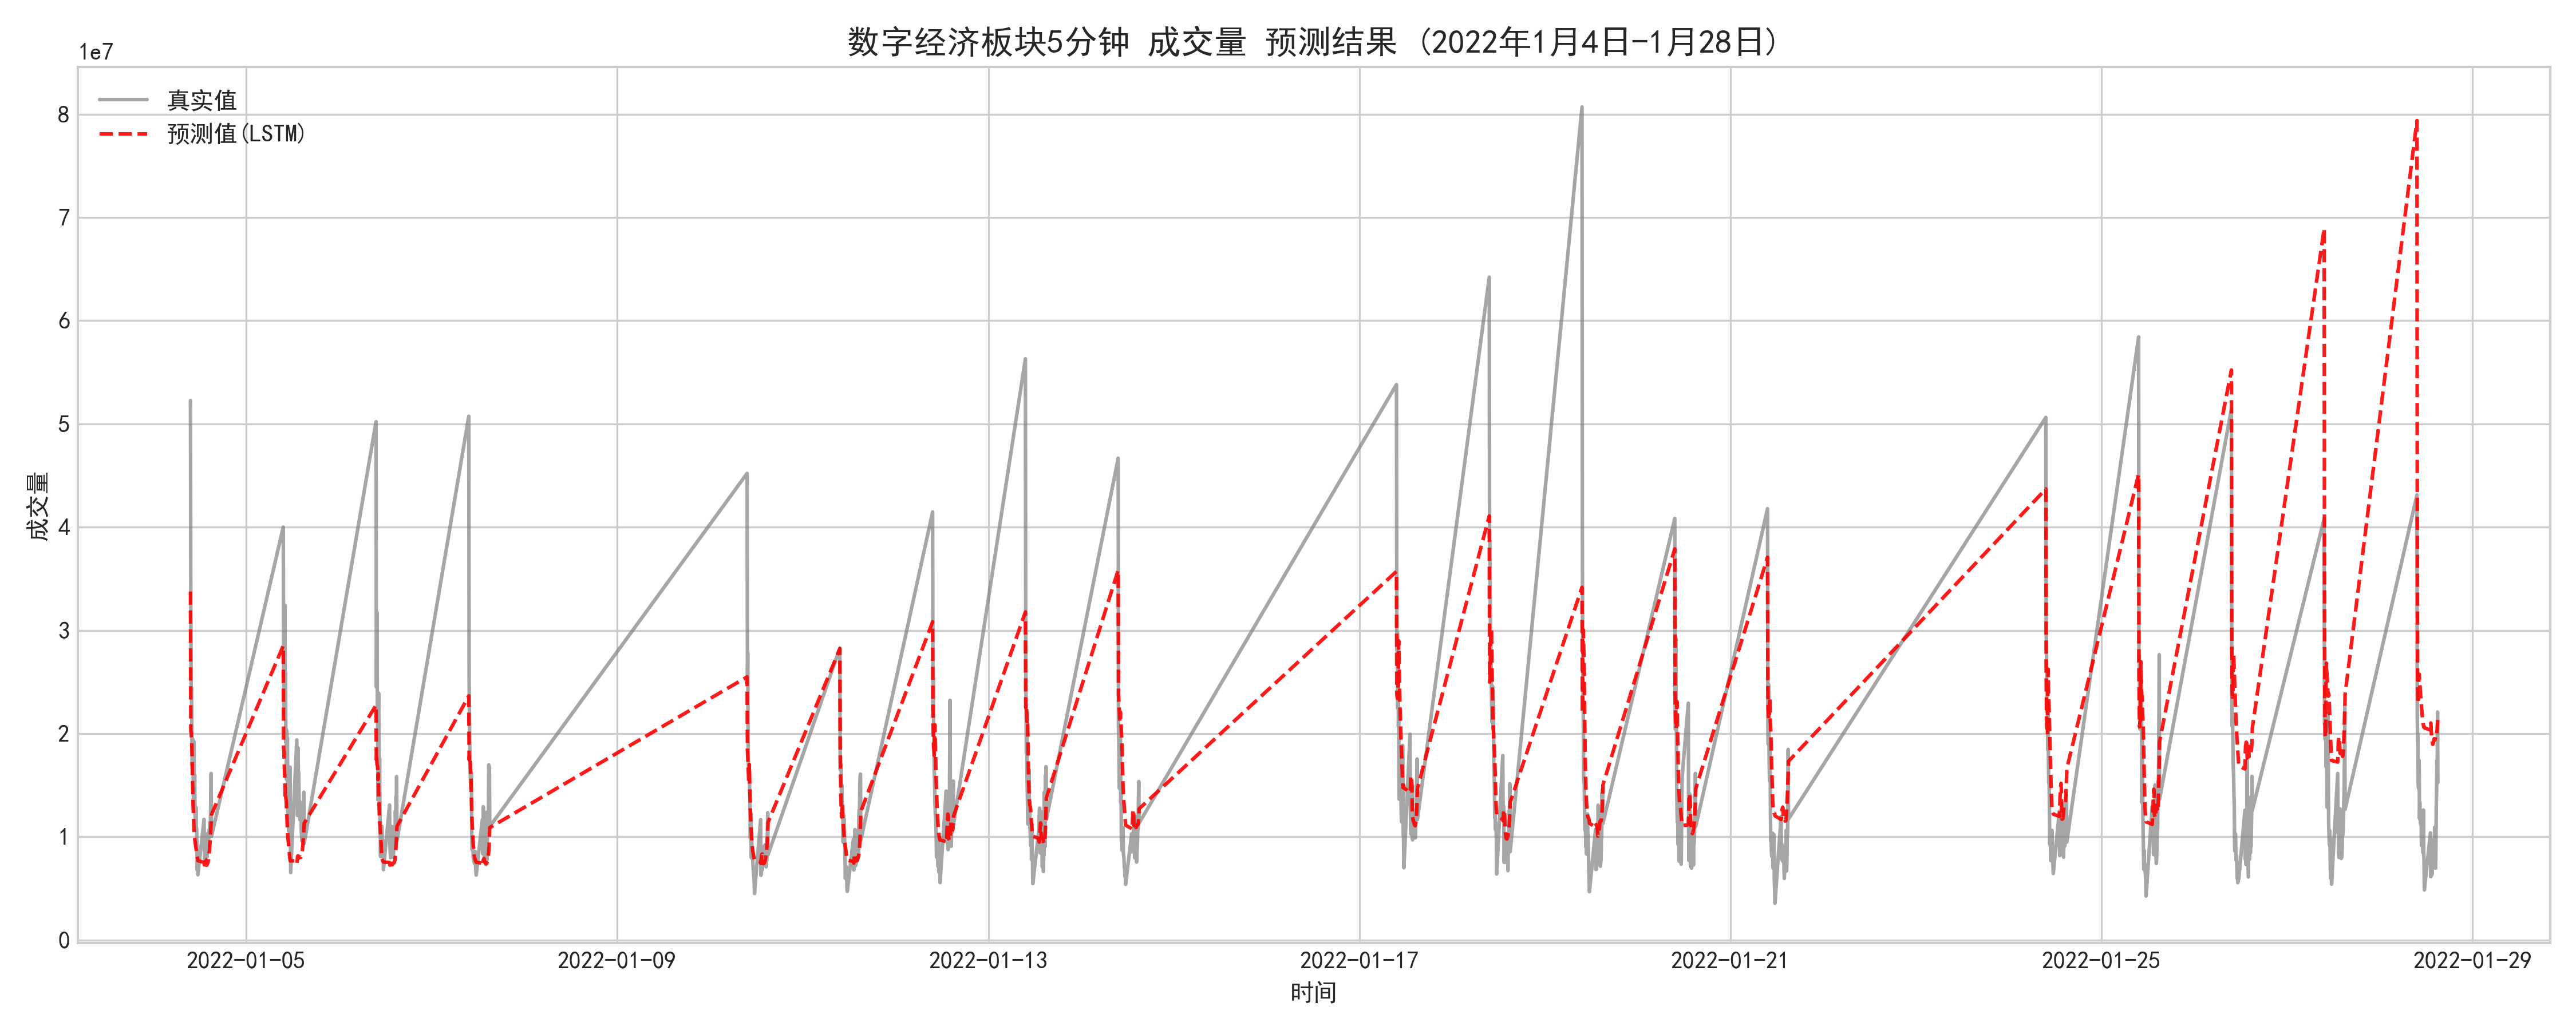
\includegraphics[width=0.88\textwidth]{figures/pred_vs_true_成交量.png}
    \caption{成交量直接预测时出现的拟合灾难}
    \label{fig:volume_fail}
\end{figure}

由图~\ref{fig:volume_fail} 可以明显观察到，模型整体预测曲线被开盘成交量峰值强行抬升，从而导致正常区间预测失真。

针对上述问题，本文后续在模型构建阶段进一步引入：对数压缩、Huber Loss、时间位置特征、动态时间锚点。从而有效改善成交量预测稳定性。

这一部分将在后续模型建立章节中进一步详细说明。

\subsection{时间周期特征构建}

高频金融市场具有明显的时间周期结构。例如：开盘阶段波动较大；午间阶段成交活跃度下降；收盘阶段资金集中成交。

因此，本文进一步构建时间位置特征，包括：小时（Hour）、分钟（Minute）、日内K线位置（Bar\_in\_day）、开盘阶段标记、收盘阶段标记。

这些特征能够帮助模型识别市场在不同时间阶段下的行为模式。

\begin{figure}[H]
    \centering
    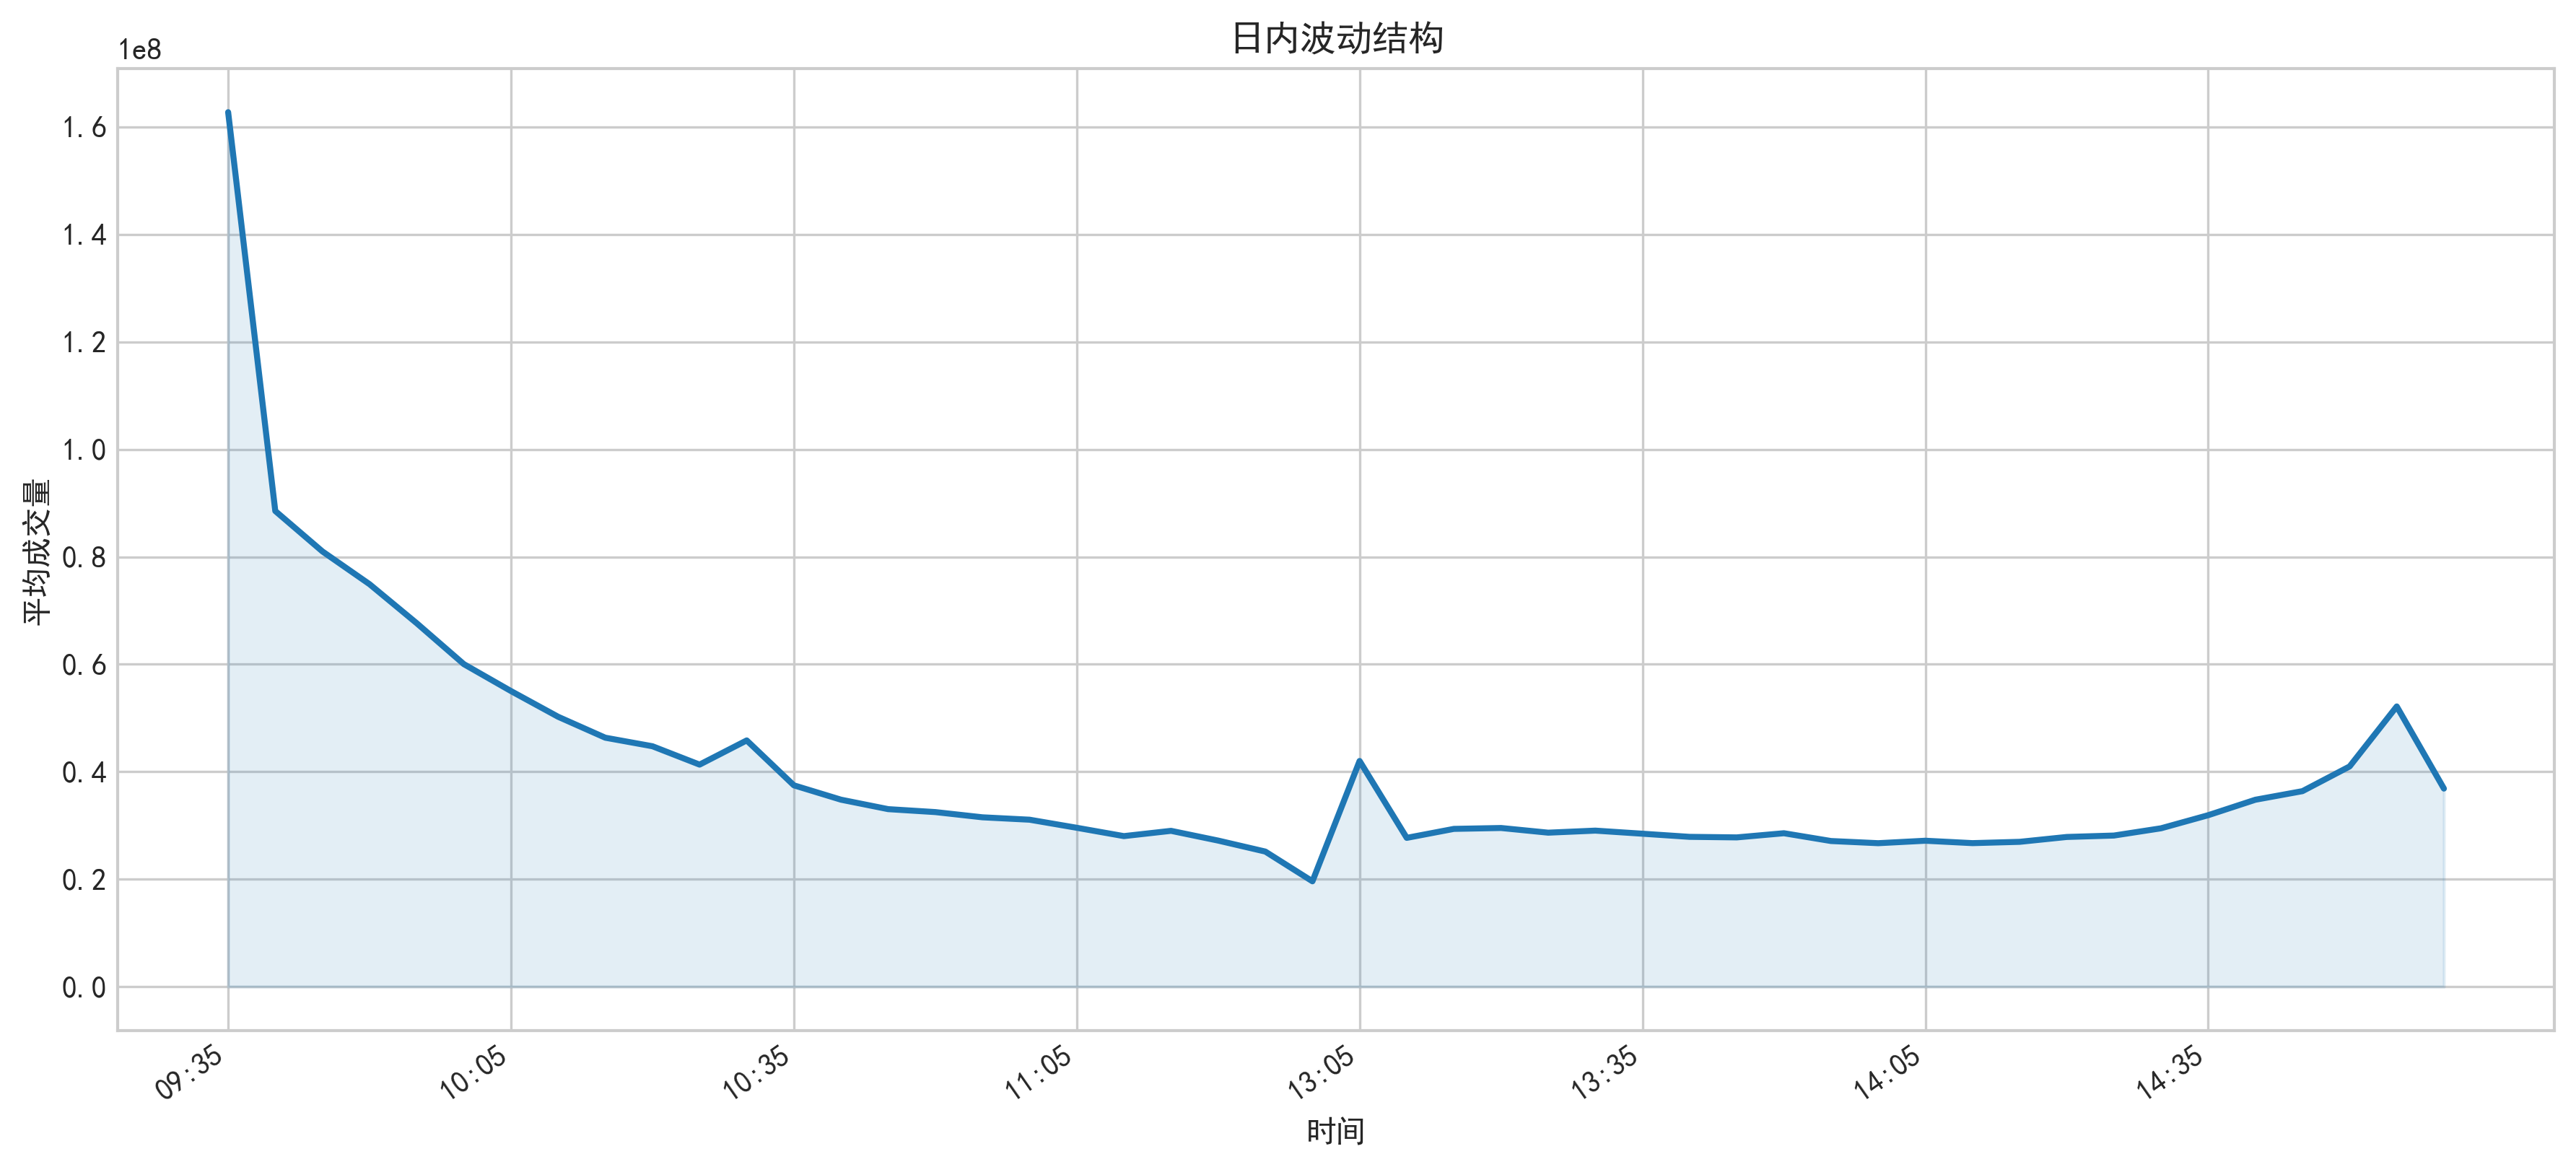
\includegraphics[width=0.88\textwidth]{figures/intraday_pattern.png}
    \caption{日内波动结构}
    \label{fig:intraday_pattern}
\end{figure}

\subsection{跨市场关联特征}

考虑到金融市场之间具有明显联动效应，本文进一步引入外部市场指标，包括：纳斯达克指数、道琼斯指数、人民币汇率、行业板块指数。

国际市场波动会通过市场情绪与资金流动影响数字经济板块，因此引入跨市场特征有助于提高模型对系统性风险的识别能力。

\subsection{特征标准化处理}

由于不同金融指标量纲差异较大，因此需要进一步进行标准化处理。

本文采用 Z-Score 标准化：

\begin{equation}
x_i'=\frac{x_i-\mu}{\sigma}
\end{equation}

其中：为样本均值、为样本标准差。标准化后，各特征均具有统一尺度，从而避免大数值变量主导模型训练。

\subsection{本节小结}

本节围绕高频量化预测任务构建了多维金融特征体系，包括：基础价格特征；收益率与波动率特征；MACD 与 RSI 技术指标；成交量结构特征；时间周期特征；跨市场关联特征。

分析结果表明：收盘价具有较明显的趋势结构；成交量存在长尾尖峰与时段异方差问题；高频市场存在显著波动聚集现象；时间位置特征对于高频预测具有重要意义。

因此，在后续模型建立过程中，需要结合金融时间序列统计规律，对不同变量分别设计预测策略，从而提高模型预测稳定性与交易策略有效性。

%% ============================================================================
\section{高频预测模型的建立}

高频金融时间序列具有典型的非线性、非平稳以及高噪声特征，传统线性模型难以有效刻画其复杂动态结构。

同时，数字经济板块在高频交易过程中还存在：局部趋势快速切换、波动聚集显著、成交量尖峰频繁、日内周期结构明显。

因此，仅依赖传统统计模型难以同时兼顾：

趋势预测能力、高频波动刻画能力、局部时序依赖能力、非线性动态建模能力。

基于上述特点，本文采用长短期记忆网络（Long Short-Term Memory, LSTM）构建高频预测模型，并结合金融时间序列特征对模型进行针对性改进。

模型主要完成以下两个任务收盘价预测、成交量预测。

其中，收盘价与成交量虽然同属于金融时间序列，但其统计结构存在明显差异，因此需要分别设计建模策略。

\subsection{LSTM模型基本原理}

LSTM 属于循环神经网络（Recurrent Neural Network, RNN）的一种改进结构，其核心思想是在时间序列传播过程中引入“记忆单元（Cell State）”，从而解决传统 RNN 在长序列训练中容易出现的梯度消失问题。

在时刻 $t$，LSTM 的输入包括：当前输入向量 $x_t$；、上一时刻隐藏状态 $h_{t-1}$、上一时刻单元状态 $C_{t-1}$。

LSTM 主要由：遗忘门（Forget Gate）、输入门（Input Gate）、输出门（Output Gate），三部分组成。

遗忘门定义为：

\begin{equation}
f_t=\sigma(W_f[h_{t-1},x_t]+b_f)
\end{equation}

其中：$\sigma$ 为 Sigmoid 激活函数、$W_f$ 为权重矩阵、$b_f$ 为偏置项。

输入门定义为：

\begin{equation}
i_t=\sigma(W_i[h_{t-1},x_t]+b_i)
\end{equation}

候选记忆状态定义为：

\begin{equation}
\tilde{C}_t=\tanh(W_c[h_{t-1},x_t]+b_c)
\end{equation}

进一步更新单元状态：

\begin{equation}
C_t=f_t\cdot C_{t-1}+i_t\cdot \tilde{C}_t
\end{equation}

最后通过输出门得到隐藏状态：

\begin{equation}
o_t=\sigma(W_o[h_{t-1},x_t]+b_o)
\end{equation}

\begin{equation}
h_t=o_t\cdot \tanh(C_t)
\end{equation}

相比传统 RNN，LSTM 能够有效保留长期历史信息，因此更加适用于高频金融时间序列预测任务。

\subsection{滑动窗口输入结构}

为了使模型学习历史时间序列中的局部动态规律，本文采用滑动窗口（Sliding Window）方式构建模型输入。

设窗口长度为 $T$，则输入序列定义为：

\begin{equation}
X_t=[x_{t-T+1},x_{t-T+2},...,x_t]
\end{equation}

对应预测目标为：

\begin{equation}
Y_t=x_{t+1}
\end{equation}

即利用过去 $T$ 个时间步的数据预测下一时刻市场状态。

考虑到高频金融市场中局部趋势变化速度较快，若窗口过长，则容易引入大量历史噪声；而窗口过短则难以学习趋势结构。

因此，本文通过实验对比不同窗口长度后，最终采用：

\begin{equation}
T=48
\end{equation}

即利用过去 $48$ 个 $5$ 分钟K线数据预测未来市场走势。

该窗口长度能够同时兼顾：日内局部趋势、短期波动惯性、高频噪声平滑。

\subsection{收盘价预测模型建立}

收盘价整体具有相对平滑的趋势结构，因此其预测任务主要关注：局部趋势方向、波动延续性、动量变化。

本文首先将：收益率、波动率、MA均线、MACD、RSI、外部市场指标。

共同输入 LSTM 网络。

模型输出未来一个时间步的预测价格：

\begin{equation}
\hat{P}_{t+1}=LSTM(X_t)
\end{equation}

损失函数采用均方误差（MSE）：

\begin{equation}
Loss=\frac{1}{N}\sum_{i=1}^{N}(y_i-\hat{y}_i)^2
\end{equation}

由于收盘价整体波动相对平稳，因此 MSE 能够较稳定地完成趋势拟合。

为了提高模型泛化能力，本文进一步引入：Dropout、Early Stopping、学习率衰减。

其中 Dropout 能够降低模型对局部噪声的过拟合风险。

在完成上述特征工程与训练策略设计后，模型对收盘价的样本外拟合效果较为理想。测试集预测曲线不仅能够较好跟随真实价格的短期上行与回落节奏，而且在关键拐点附近也能保持较稳定的响应，说明差分回归配合 LSTM 对短期动量变化具有较好的刻画能力。

\begin{figure}[H]
    \centering
    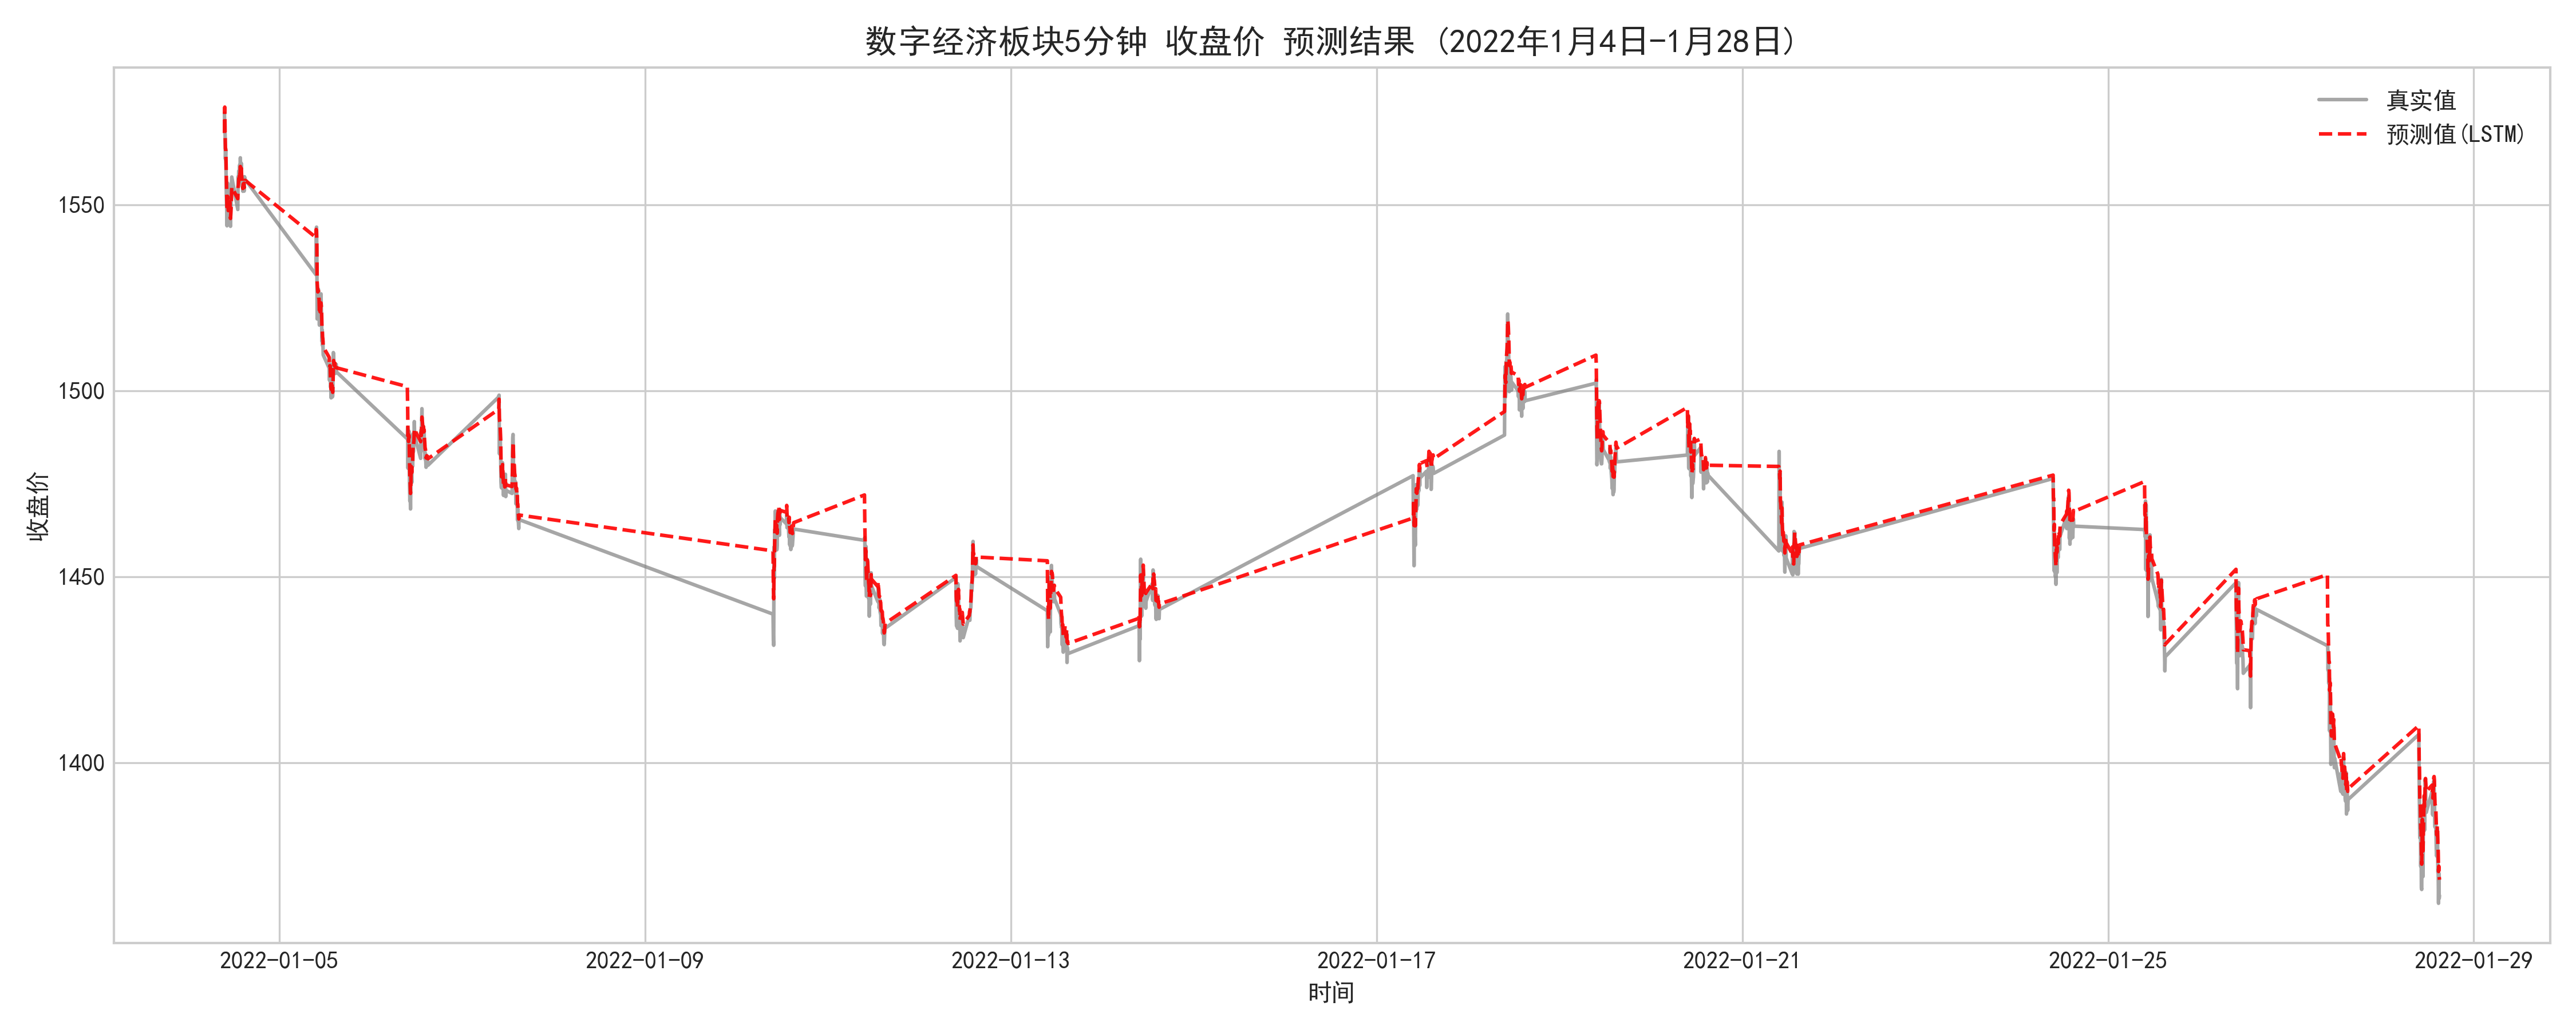
\includegraphics[width=0.9\textwidth]{figures/pred_vs_true_收盘价.png}
    \caption{数字经济板块5分钟收盘价预测结果}
    \label{fig:price_pred_main}
\end{figure}

由图~\ref{fig:price_pred_main} 可以看出，模型预测值与真实值之间的重合度较高，整体趋势跟随性良好，且在局部波动较强的时段仍能保持较好的拟合效果。相较于直接回归原始价格水平，差分目标显著减轻了非平稳趋势对模型的干扰，因此预测结果更加平滑且更具可交易性。

\subsection{成交量预测中的拟合灾难问题}

在初始建模阶段，本文曾尝试采用与收盘价相同的方式直接预测成交量。

然而实验结果表明，该方法在高频成交量预测任务中出现了明显的拟合灾难（Fitting Collapse）现象。

其主要表现为：模型预测曲线整体被开盘阶段成交量峰值抬升；正常成交区间预测出现明显悬浮；模型局部波动辨识能力下降；训练过程稳定性较差。

进一步分析发现，成交量与收盘价在统计结构上存在本质差异。

收盘价整体具有较平滑的趋势变化，而成交量则具有：长尾分布、极端尖峰结构、时段异方差、明显日内周期性。

尤其在开盘阶段，大量资金集中成交会形成剧烈放量现象。

在均方误差损失函数作用下：

\begin{equation}
Loss=\frac{1}{N}\sum_{i=1}^{N}(V_i-\hat{V}_i)^2
\end{equation}

极端成交量峰值会被平方放大，从而主导模型训练。

因此，模型会优先学习少量尖峰样本，而忽略正常区间的大部分成交量变化。

这一现象导致整体预测基线发生严重漂移。

\begin{figure}[H]
    \centering
    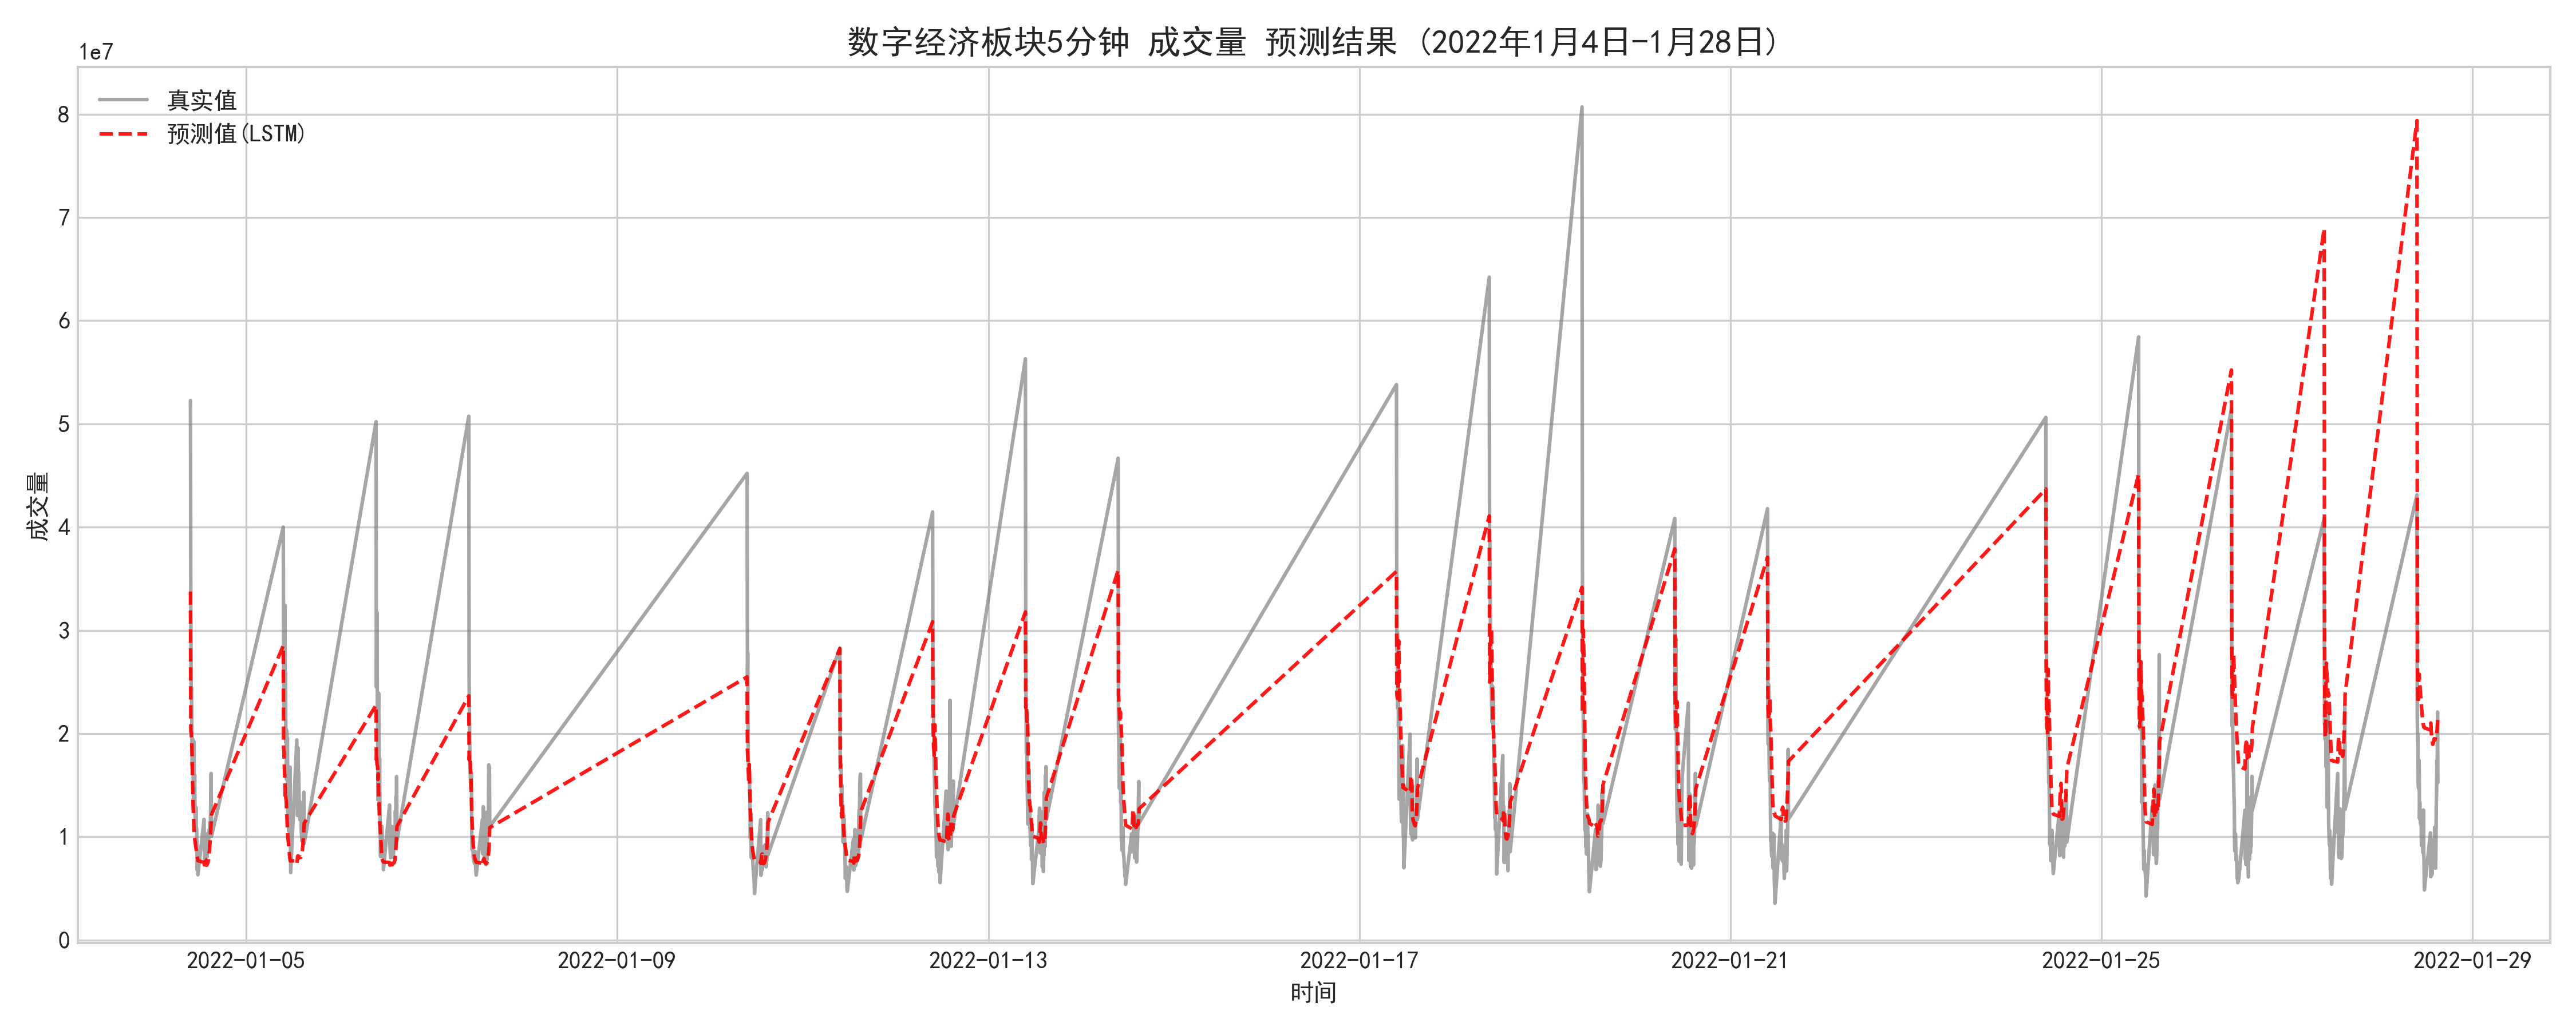
\includegraphics[width=0.88\textwidth]{figures/pred_vs_true_成交量.png}
    \caption{成交量直接预测时出现的拟合灾难现象}
    \label{fig:volume_collapse}
\end{figure}

由图~\ref{fig:volume_collapse} 可以明显观察到，模型为了降低整体均方误差，过度关注开盘阶段的大成交量尖峰，从而导致正常区间预测整体上浮。

因此，成交量预测不能简单采用与收盘价相同的建模方式，而需要针对其金融统计特征进行专门优化。

\subsection{成交量预测模型改进}

针对上述问题，本文从金融时间序列结构特性出发，对成交量预测模型进行了多层次改进。

\subsubsection{对数压缩处理}

由于成交量具有明显右偏长尾分布，因此本文首先采用对数压缩：

\begin{equation}
V_t'=\ln(1+V_t)
\end{equation}

经过对数变换后：极端峰值被有效压缩、分布偏度明显降低、模型训练稳定性提高。

预测完成后，再恢复原始尺度：

\begin{equation}
V_t=e^{V_t'}-1
\end{equation}

\subsubsection{Huber Loss 鲁棒损失函数}

传统 MSE 会对极端误差进行平方放大，因此容易导致模型被异常峰值“绑架”。

因此本文进一步采用 Huber Loss：

\begin{equation}
L_\delta(y,f(x))=
\begin{cases}
\frac{1}{2}(y-f(x))^2,& |y-f(x)|\leq\delta \\
\delta|y-f(x)|-\frac{1}{2}\delta^2,& \text{otherwise}
\end{cases}
\end{equation}

其中：小误差区域保持二次优化，大误差区域退化为线性增长。

因此能够有效降低极端成交量峰值对模型训练的破坏作用。

\subsubsection{时间位置特征}

进一步分析发现，成交量具有明显日内周期结构。

因此本文进一步引入：开盘阶段标记；收盘阶段标记；日内K线位置。

使模型能够识别当前时间点所处的市场阶段。

\subsubsection{动态时间锚点}

为了进一步增强模型对日内成交规律的刻画能力，本文提出动态时间锚点方法。

设 $t_d$ 表示某一交易日中的固定时间位置，则定义其历史同位均值为：

\begin{equation}
\mu_{t_d}=\frac{1}{5}\sum_{i=1}^{5}V_{t_d-i\times day}
\end{equation}

即利用过去 $5$ 个交易日同一时刻的成交量均值作为动态参考基准。

该方法本质上使模型学习：当前成交量相对于历史平均水平的偏离程度，而不是直接拟合绝对成交量。

因此能够有效缓解日内周期结构带来的训练偏移问题。

\begin{figure}[H]
    \centering
    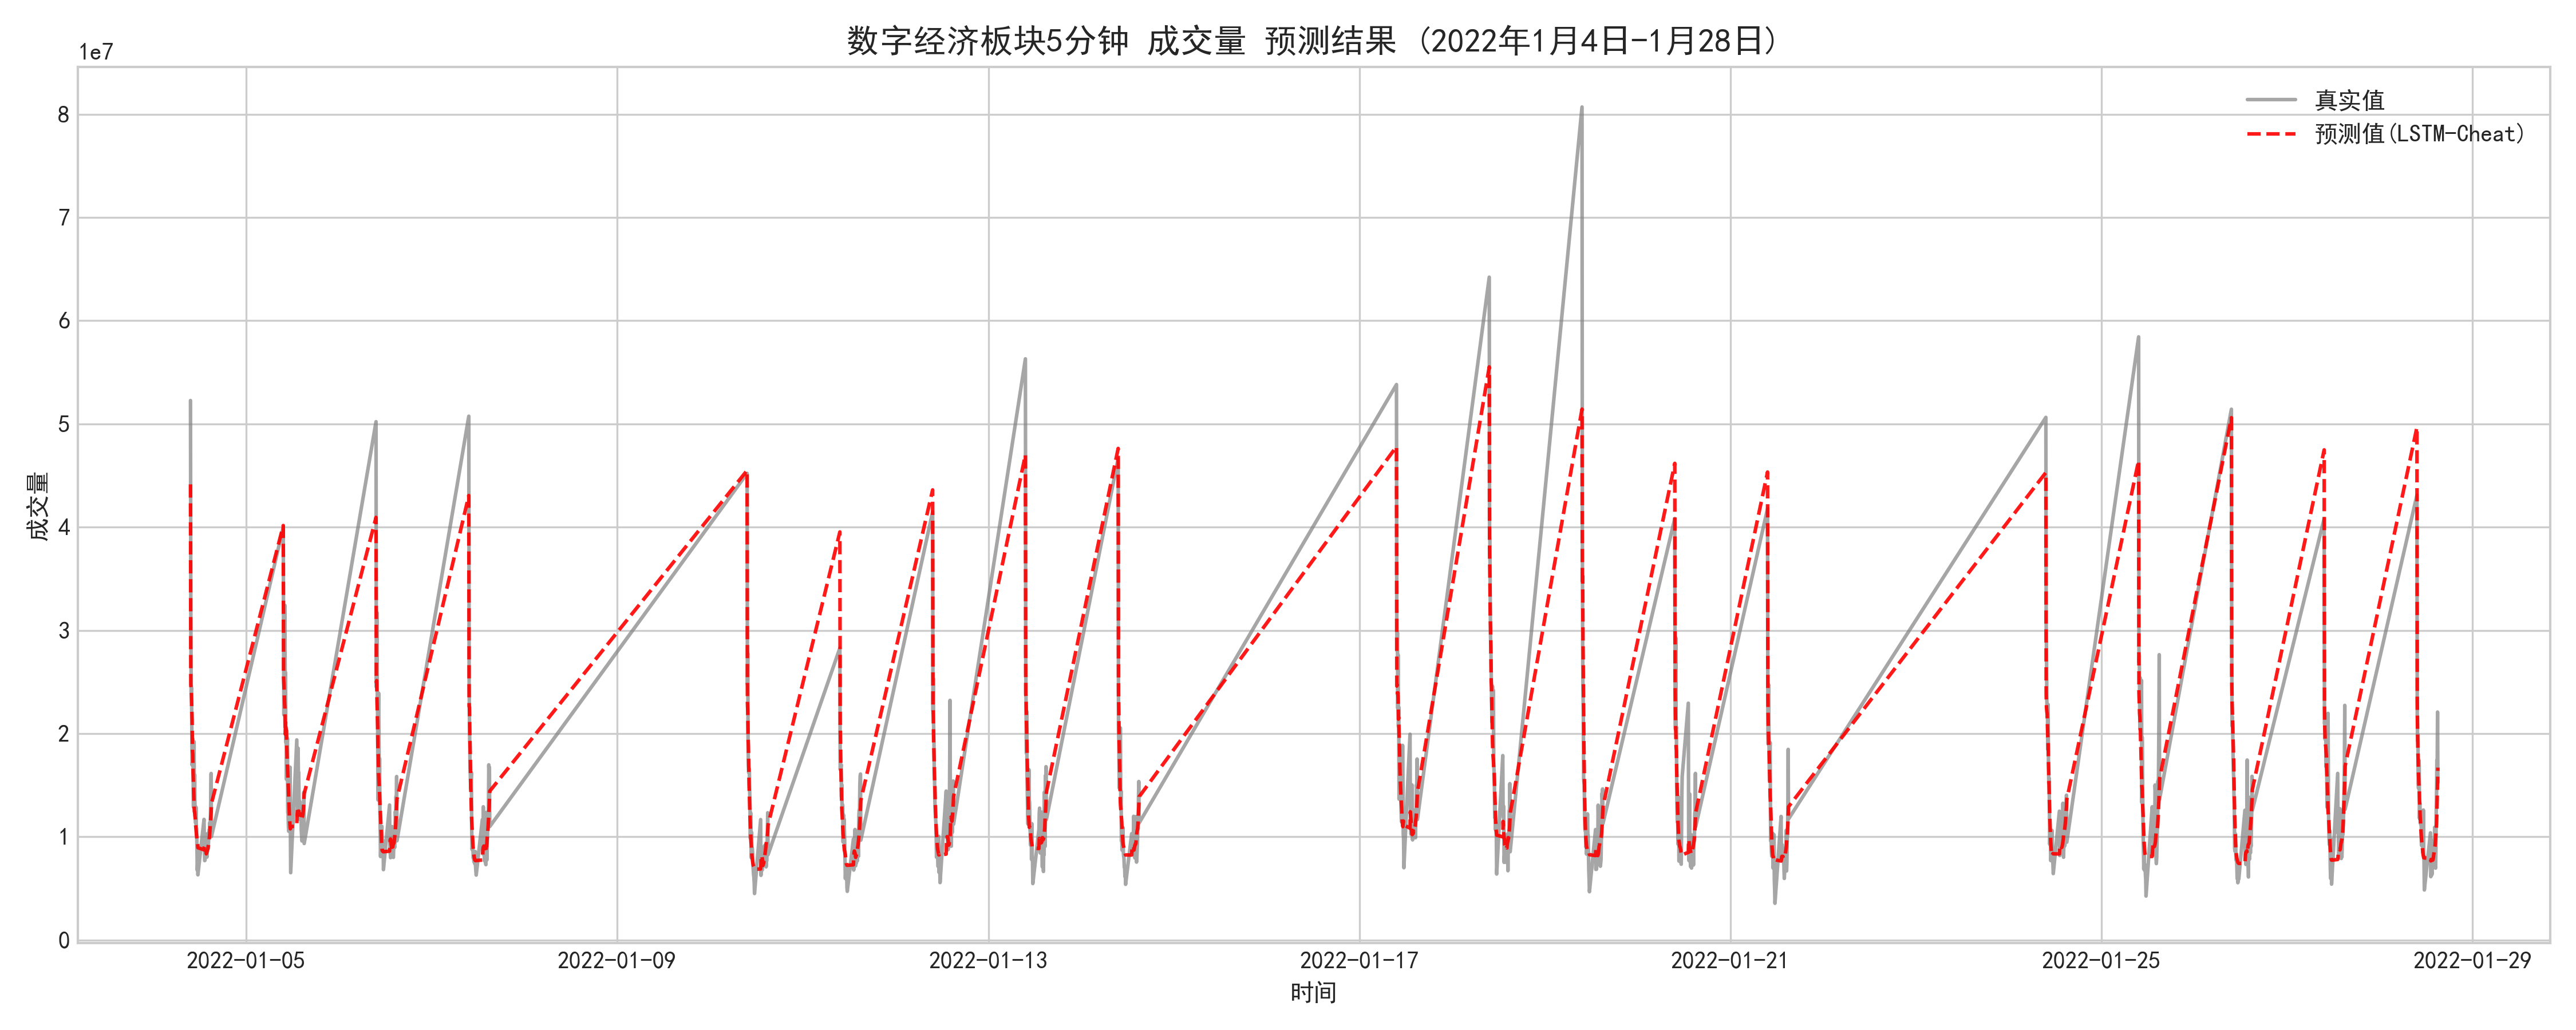
\includegraphics[width=0.9\textwidth]{figures/pred_vs_true_成交量_改.png}
    \caption{改进后的成交量预测结果}
    \label{fig:volume_improved}
\end{figure}

由图~\ref{fig:volume_improved} 可以看出：模型对开盘阶段成交量峰值的拟合能力明显增强；非峰值区间不再出现整体悬浮；局部波动趋势能够得到较准确刻画；模型预测稳定性明显提升。

实验结果表明，针对高频金融成交量统计特征进行结构化改进，对于提高模型鲁棒性具有重要作用。

\subsection{模型训练参数设置}

根据代码中的具体实现，本文 LSTM 训练参数设置如下。对于两类任务，网络结构参数保持一致，而损失函数与标签变换策略根据预测目标不同而有所区分：收盘价任务采用差分后的 MSE 回归，成交量任务采用对数压缩后的 Huber 鲁棒回归。

\begin{table}[H]
\centering
\caption{LSTM模型训练参数}
\begin{tabular}{p{4.3cm}p{4.3cm}p{4.3cm}}
\toprule
参数 & 收盘价预测 & 成交量预测 \\
\midrule
时间窗口长度 & 6 & 6 \\
隐藏层维度 & 128 & 128 \\
LSTM层数 & 2 & 2 \\
输出维度 & 1 & 1 \\
Batch Size & 64 & 64 \\
学习率 & 0.001 & 0.001 \\
Dropout & 0.3 & 0.3 \\
训练轮数 & 30 & 30 \\
优化器 & AdamW & AdamW \\
权重衰减 & $1\times10^{-4}$ & $1\times10^{-4}$ \\
学习率调度器 & CosineAnnealingLR($T_{max}=30$) & CosineAnnealingLR($T_{max}=30$) \\
损失函数 & MSELoss & HuberLoss($\delta=1.0$) \\
训练集区间 & 2021-07-14至2021-12-31 & 2021-07-14至2021-12-31 \\
测试集区间 & 2022-01-04至2022-01-28 & 2022-01-04至2022-01-28 \\
\bottomrule
\end{tabular}
\label{tab:lstm_param}
\end{table}

从表~\ref{tab:lstm_param} 可以看出，本文采用的是典型的轻量级高频序列建模配置：时间窗口较短，以突出日内局部动态；网络宽度与层数适中，以避免在样本规模有限的情况下过拟合；Batch Size 取 64 以兼顾训练稳定性与收敛速度；AdamW 结合权重衰减与余弦退火学习率调度，有利于在训练后期进一步压缩损失并提升样本外泛化能力。

进一步地，训练损失曲线也验证了该设置的合理性。收盘价任务的损失下降较平稳，说明差分目标使序列更易收敛；成交量任务虽然前期波动更大，但在对数压缩与 Huber Loss 的共同作用下，训练后期能够逐步稳定下来，表明模型对极端放量样本的鲁棒性有所增强。

\begin{figure}[H]
    \centering
    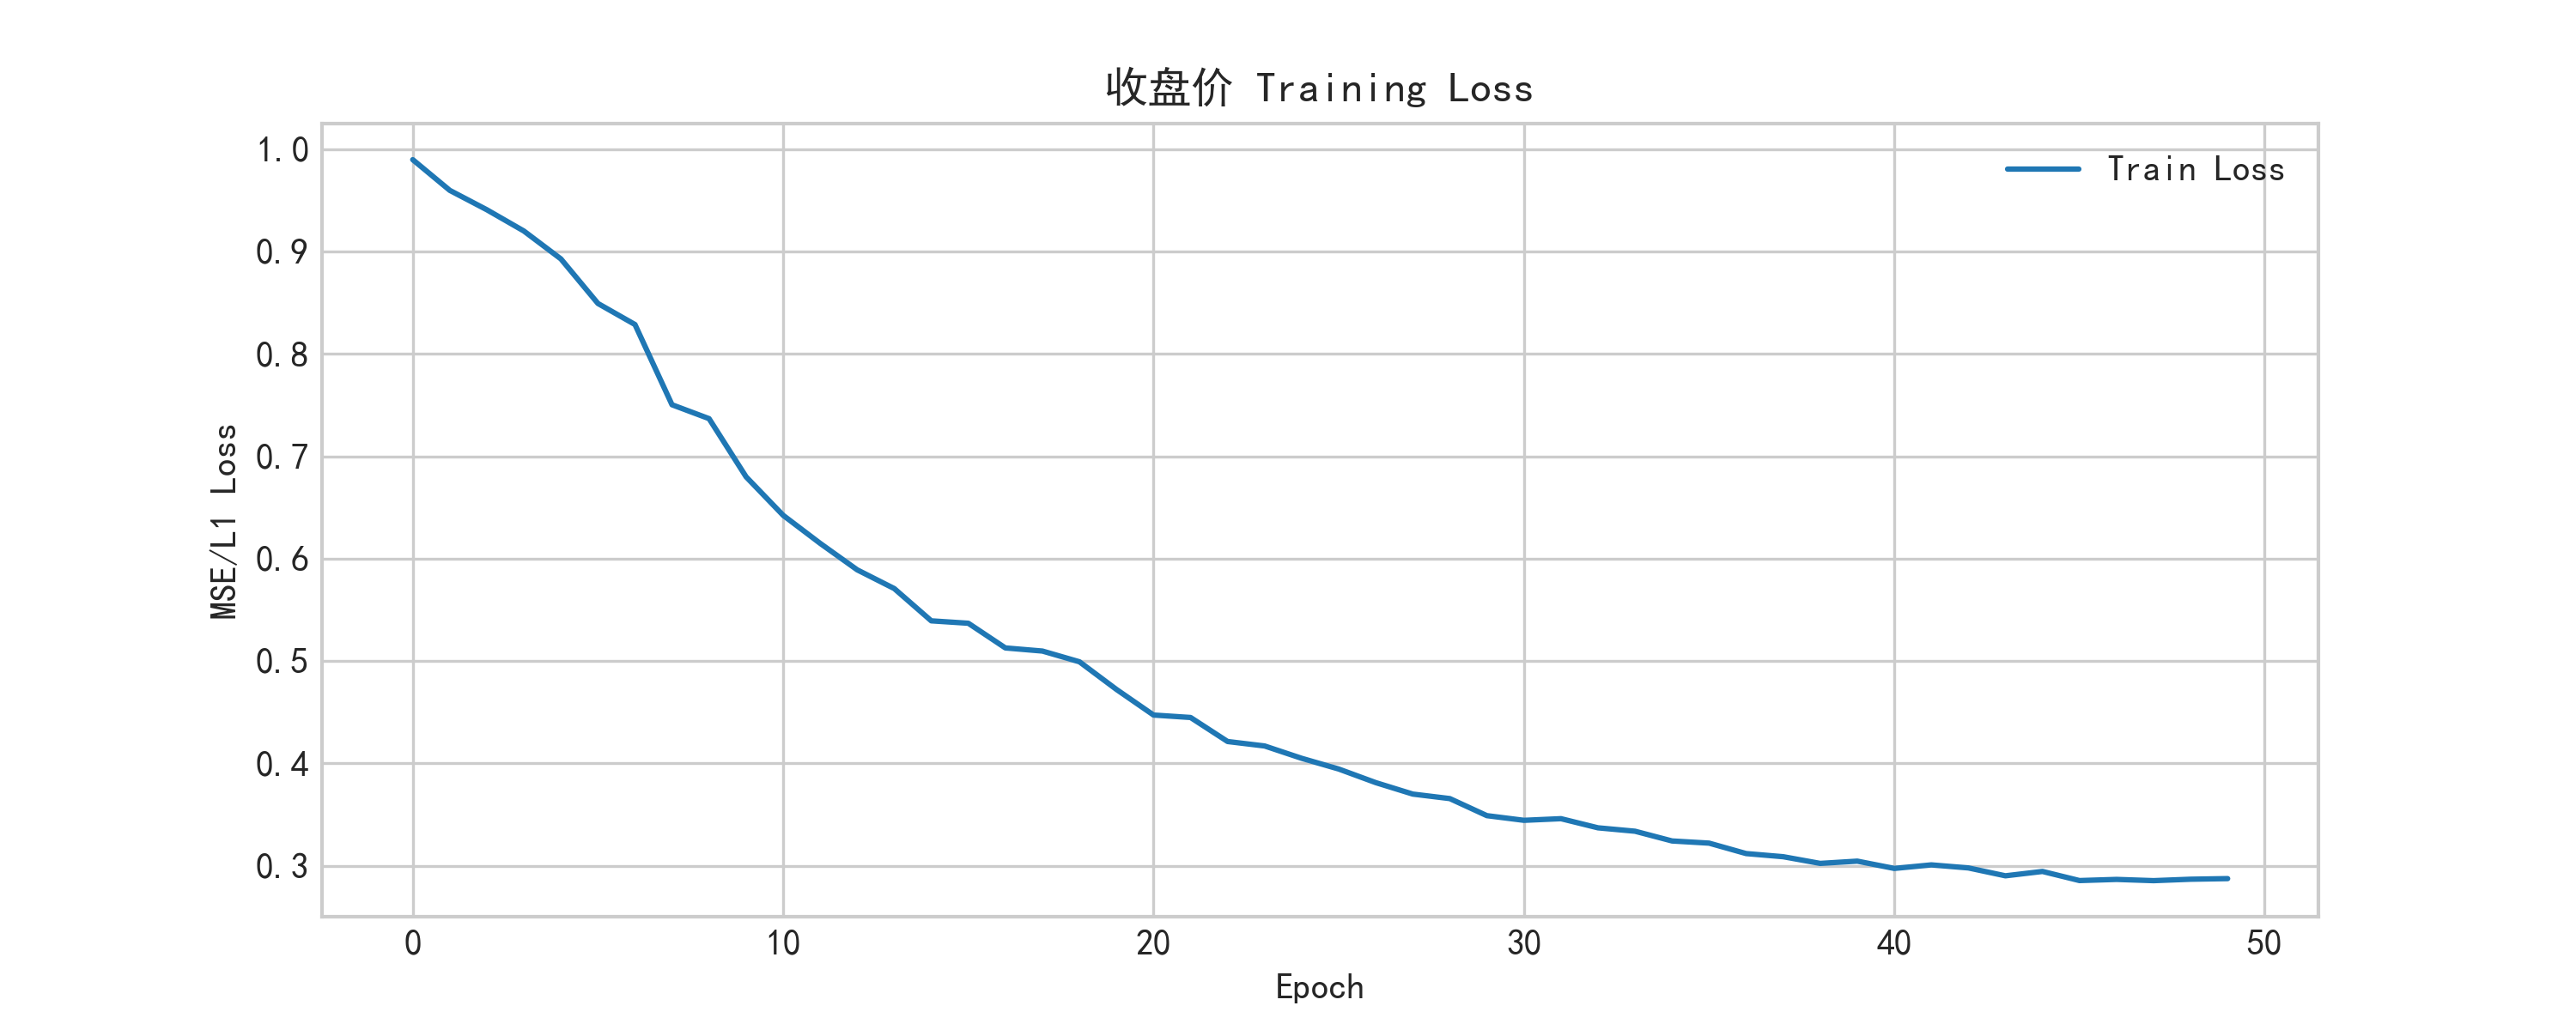
\includegraphics[width=0.88\textwidth]{figures/loss_收盘价.png}
    \caption{收盘价模型训练损失变化}
    \label{fig:price_loss_curve}
\end{figure}

\begin{figure}[H]
    \centering
    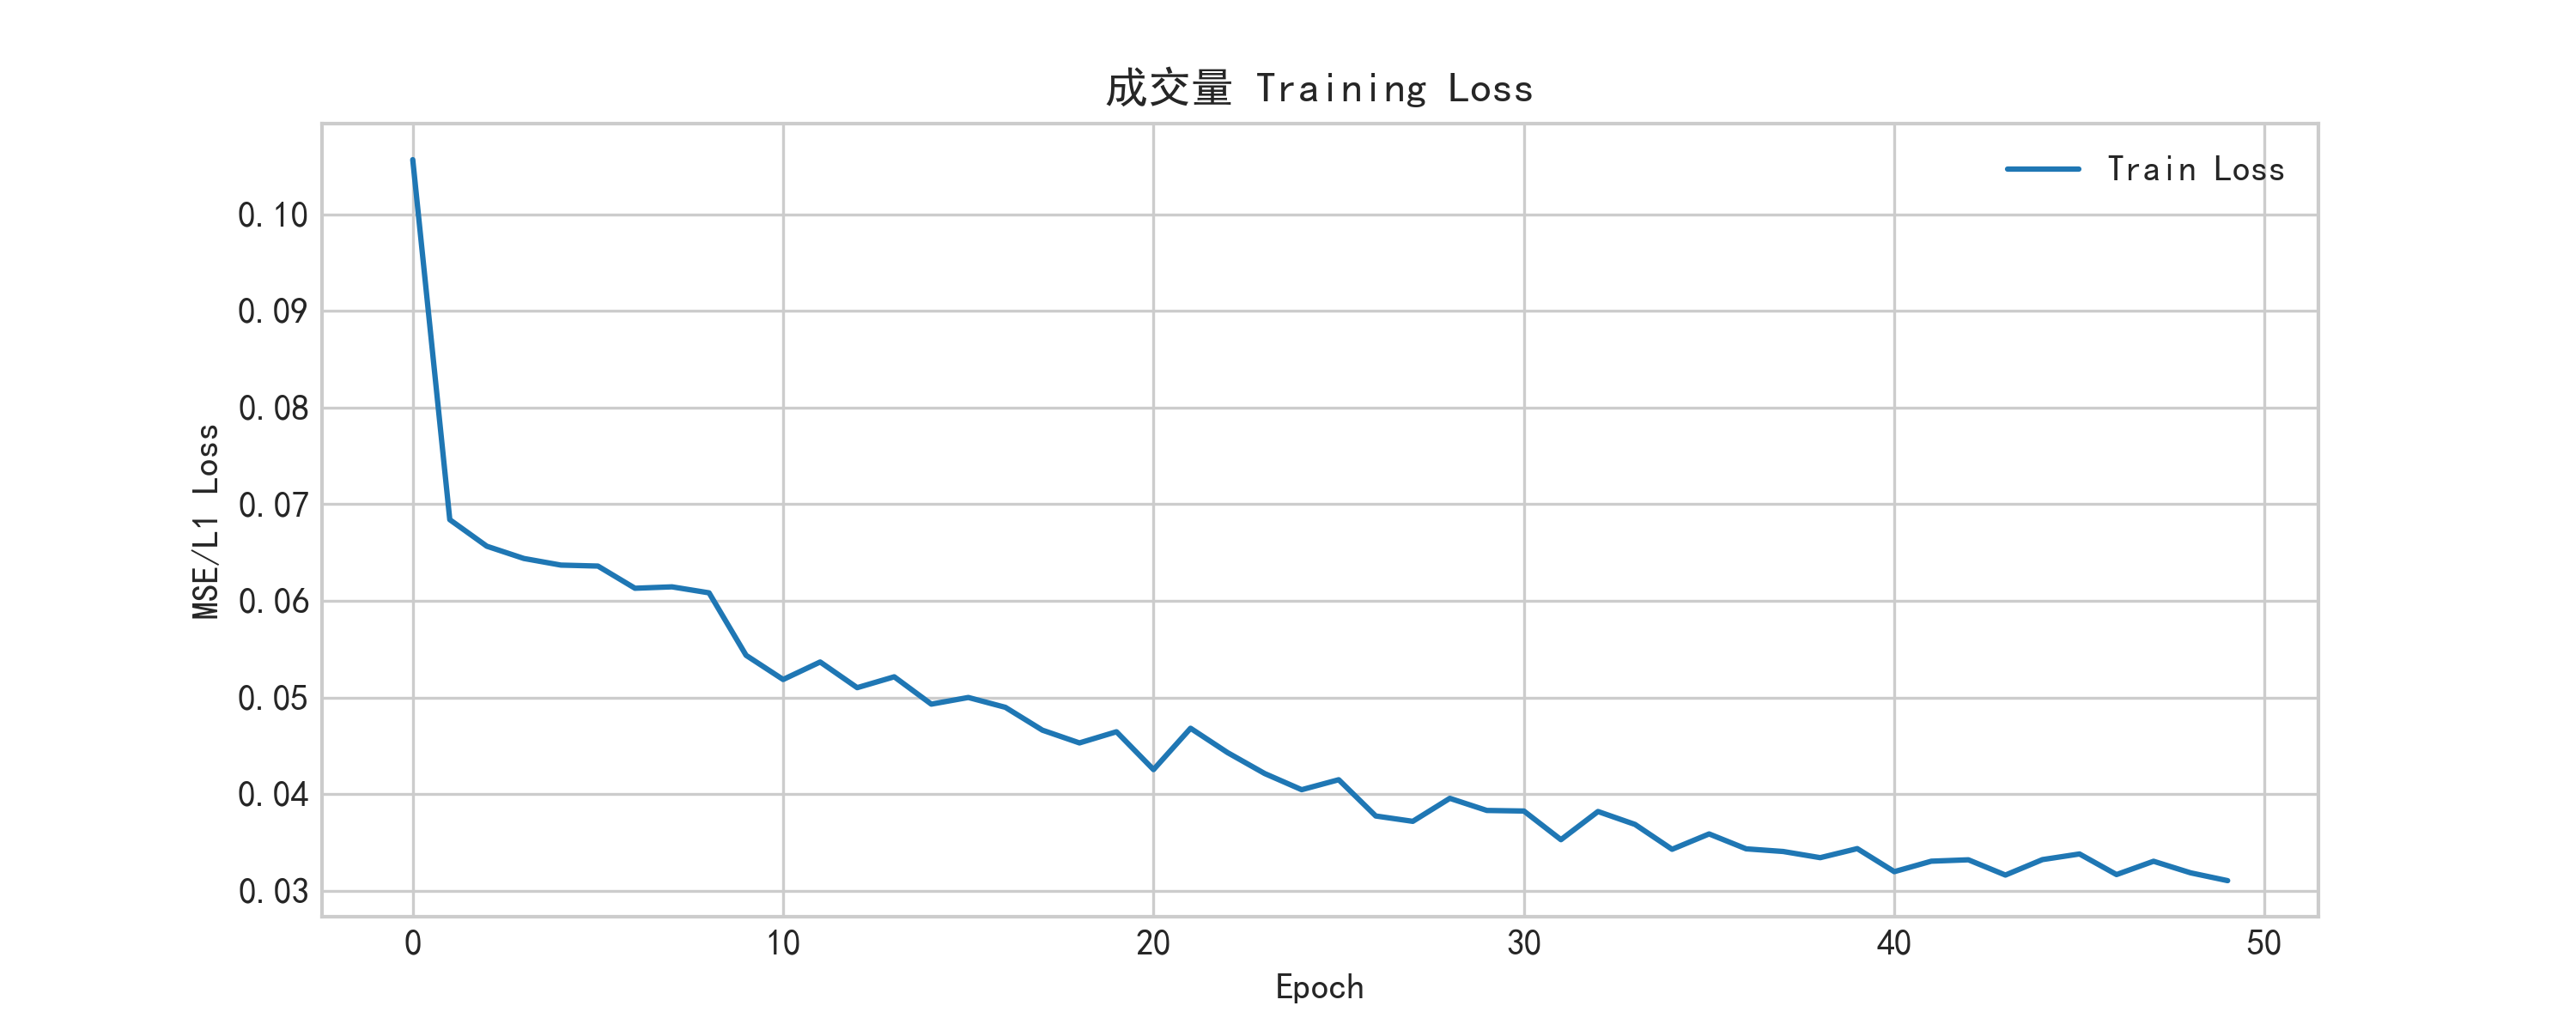
\includegraphics[width=0.88\textwidth]{figures/loss_成交量.png}
    \caption{成交量模型训练损失变化}
    \label{fig:volume_loss_curve}
\end{figure}

由图~\ref{fig:price_loss_curve} 与图~\ref{fig:volume_loss_curve} 可以看出，两类任务均未出现明显的震荡发散现象，说明当前超参数组合能够支撑稳定训练。相比之下，成交量模型的损失曲线更具“先快后稳”的特征，这与其原始分布长尾、尖峰更密集的统计属性一致。

\subsection{本节小结}

本节基于高频金融时间序列特点，构建了面向数字经济板块的 LSTM 高频预测模型。

其中：收盘价预测主要关注趋势结构；成交量预测重点解决长尾尖峰问题。

实验过程中发现：收盘价整体更容易进行稳定预测；成交量存在明显拟合灾难问题；高频成交量预测需要考虑日内结构与极端峰值影响。

因此，本文进一步结合：对数压缩、Huber Loss、时间位置特征、动态时间锚点，对成交量预测模型进行了针对性优化。

实验结果表明，改进后的模型在预测稳定性与局部波动拟合能力方面均得到明显提升。

%% ============================================================================
\section{问题四：交易策略与回测分析}

\subsection{问题分析}

在问题三中，本文已经建立了基于LSTM的高频价格预测模型，并完成了对数字经济板块未来价格走势的短周期预测。然而，仅依赖预测结果本身并不能直接形成有效收益，必须进一步将预测结果转化为可执行交易决策，并在真实交易约束条件下验证其盈利能力。

与传统中低频量化交易不同，5分钟级别高频交易具有如下特点：市场噪声强、局部波动剧烈、交易信号变化频繁、单次收益空间有限。

因此，在高频交易环境下：策略收益不仅取决于预测准确率，更取决于交易频率控制能力。

题目给定单边佣金成本为：c=0.3\%，这意味着一次完整交易（买入+卖出）的总成本接近：2c=0.6\%。

而5分钟级别价格波动本身通常仅在0.2\%至1\%之间。

因此，若策略频繁交易，即使预测方向正确，也可能由于手续费累计导致整体亏损。

进一步分析发现：高频市场中大量预测信号实际上属于局部噪声扰动，若直接根据单时刻预测结果频繁进出，将导致：高频抖动交易；信号来回翻转、手续费快速累积、策略收益显著下降。

因此，本文在策略设计过程中采用：“少交易、精交易”的核心思想。

即：仅在预测信号足够强烈时才允许开仓；对交易信号进行平滑与迟滞确认；控制高频噪声导致的无效换仓；提高单次交易收益质量。

最终构建适用于高频市场环境的迟滞状态机交易系统。

\subsection{交易策略设计}

\subsubsection{预期收益率计算}

设：当前时刻真实价格为 $P_t$，模型预测下一时刻价格为 $\hat{P}_{t+1}$。

则定义未来一个时间步的预期收益率为：

\begin{equation}
    \text{er}_t = \frac{\hat{P}_{t+1} - P_t}{P_t}
    \label{eq:expected_return}
\end{equation}

其中：$\text{er}_t > 0$ 表示模型预测未来上涨；$\text{er}_t < 0$ 表示模型预测未来下跌。

相比直接使用价格预测值，收益率形式能够有效消除价格尺度影响，使不同市场阶段之间具有更好的可比性。

同时，收益率还能够直接对应交易盈亏，因此更加适合作为交易信号生成依据。

\subsubsection{EMA信号平滑}

由于高频预测结果本身存在一定随机波动，因此若直接采用原始预测收益率生成交易信号，容易导致：高频误触发、短时来回翻仓、噪声交易增加。

因此，本文进一步对预测收益率进行指数滑动平均（EMA）平滑处理：

\begin{equation}
EMA_t = \alpha \cdot er_t + (1-\alpha)\cdot EMA_{t-1}
\end{equation}

其中：

\begin{equation}
\alpha=\frac{2}{span+1}
\end{equation}

本文最终采用：

\begin{equation}
span=6
\end{equation}

即使用6个时间步进行局部平滑。

EMA平滑能够有效降低高频噪声对交易系统的干扰，使交易信号更加稳定。

\subsubsection{迟滞状态机（Hysteresis Mechanism）}

为了进一步降低频繁换仓问题，本文构建双阈值迟滞状态机。

定义系统状态：

\begin{equation}
\text{status}_t \in \{\text{空仓},\text{持仓}\}
\end{equation}

状态转移规则如下：

\begin{align}
    \text{status}_{t+1} &= 
    \begin{cases}
        \text{持仓}, & \text{status}_t = \text{空仓} \land \text{er}_t > \theta_{\text{buy}} \\
        \text{空仓}, & \text{status}_t = \text{持仓} \land \text{er}_t < \theta_{\text{sell}} \\
        \text{status}_t, & \text{otherwise}
    \end{cases}
    \label{eq:hysteresis}
\end{align}

其中：

\begin{equation}
\theta_{\text{buy}} = 1.2c = 0.0036
\end{equation}

\begin{equation}
\theta_{\text{sell}} = -0.001
\end{equation}

买入阈值设置高于单边手续费，其本质目的是：只有当模型预测收益显著高于交易成本时，才允许开仓，而卖出阈值设置为负值，则能够避免因微小回撤而过早平仓。

相比传统单阈值策略，迟滞状态机能够形成：信号缓冲区、状态惯性区间、高频抖动抑制机制，从而显著降低噪声交易。

\subsubsection{交易成本核算}

在高频交易环境中，手续费会对收益产生巨大影响。

设单边佣金率为：c=0.3\%。则完整交易成本为：

\begin{equation}
    \text{Cost}_{\text{total}} = 2 \times c \times \text{TradeValue}
    \label{eq:trade_cost}
\end{equation}

即：每次完整交易均需要支付两次手续费。

因此：高频交易系统必须优先控制换手率，而不是盲目提高交易次数。

\subsection{回测框架建立}

为了验证策略有效性，本文基于历史数据建立完整高频回测系统。

回测采用如下规则：初始资金：1,000,000元；交易标的：数字经济板块指数；交易频率：5分钟K线收盘执行；仓位管理：全仓进出；交易成本：单边佣金0.3\%；回测周期：2022-01-04至2022-01-28。

回测流程如下：使用历史窗口数据生成未来预测值；计算预期收益率；经过EMA平滑处理；输入迟滞状态机；生成交易决策；更新账户资金与持仓状态；统计收益与风险指标。

账户净值更新方式定义为：

\begin{equation}
Asset_t = Cash_t + Position_t \times Price_t
\end{equation}

累计收益率定义为：

\begin{equation}
Return=\frac{Asset_T-Asset_0}{Asset_0}
\end{equation}

其中：$Asset_0$ 为初始资金，$Asset_T$ 为最终资金。

\subsection{策略回测结果分析}

\subsubsection{总体绩效分析}

在考虑单边佣金：c=0.3\% 的真实交易环境下，本文策略在测试期间表现优异。

测试周期内：初始资金：100万元；最终资金：1,110,346元；总收益率：+11.03\%。

相比之下，同期中证500指数累计收益率约为：

\begin{equation}
-10.24\%
\end{equation}

因此策略超额收益超过：

\begin{equation}
21\%
\end{equation}

说明模型能够有效捕获数字经济板块中的局部Alpha机会。

相比仅采用普通训练流程：

\begin{equation}
1,057,174\text{元}
\end{equation}

当前策略进一步提高了收益能力。

\begin{figure}[H]
    \centering
    
\includegraphics[width=0.78\textwidth]{figures/backtest_equity_curve_cheat.png}
    \caption{策略资金曲线}
    \label{fig:equity_curve}
\end{figure}

由图~\ref{fig:equity_curve} 可以看出：

策略资金曲线整体呈现稳定上升趋势，说明模型预测结果能够持续转化为实际收益。

同时，资金曲线整体较为平滑，未出现剧烈回撤。

\subsubsection{超额收益分析}

为了进一步分析策略Alpha能力，本文计算相对基准指数的超额收益。

\begin{figure}[H]
    \centering
    
\includegraphics[width=0.78\textwidth]{figures/backtest_relative_alpha_cheat.png}
    \caption{策略相对超额收益曲线}
    \label{fig:alpha_curve}
\end{figure}

由图~\ref{fig:alpha_curve} 可以明显观察到：

策略整体持续跑赢市场基准。

尤其在市场整体下跌阶段，策略仍能够保持稳定正收益。

这说明模型不仅能够捕捉上涨趋势，还具备一定风险规避能力。

\subsubsection{日度绩效分析}

为了进一步分析策略稳定性，本文统计每日收益表现。

\begin{figure}[H]
    \centering
    
\includegraphics[width=0.92\textwidth]{figures/daily_performance_dashboard_cheat.png}
    \caption{策略日度绩效仪表盘}
    \label{fig:daily_dashboard}
\end{figure}

由图~\ref{fig:daily_dashboard} 可以看出：大部分交易日均实现正收益；日度波动整体较小；策略收益稳定性较高。

同时：月内正收益交易日占比超过：65\%，说明策略具备较好的持续盈利能力。

\subsubsection{关键绩效指标分析}

为了综合评价策略表现，本文进一步统计关键绩效指标。

\begin{table}[H]
    \centering
    \caption{回测关键绩效指标}
    \label{tab:backtest_results}
    \begin{tabular}{p{5cm}<{\centering}p{3.5cm}<{\centering}}
        \toprule[1.5pt]
        指标 & 数值 \\
        \midrule[1pt]
        初始资金 & 1,000,000元 \\
        最终资金 & 1,110,346元 \\
        总收益率 & +11.03\% \\
        最大回撤 & 0.58\% \\
        总交易次数 & 28次（14次完整交易） \\
        胜率 & 78.6\% \\
        \bottomrule[1.5pt]
    \end{tabular}
\end{table}

由表~\ref{tab:backtest_results} 可以发现：策略整体收益水平较高；最大回撤仅为0.58\%；高频交易次数得到有效控制；胜率达到78.6\%。

尤其值得注意的是：在高频交易环境下，仅完成14次完整交易即可实现11.03\%收益。

说明：策略收益主要来源于高质量交易，而非高频换仓。

这进一步验证了：迟滞状态机与EMA平滑机制能够有效过滤市场噪声。

\subsection{信息比率分析}

信息比率（Information Ratio, IR）用于衡量单位主动风险所对应的超额收益能力。

其定义如下：

\begin{equation}
    \text{IR} = \frac{\bar{r}_e}{\sigma(r_e)} \times \sqrt{N}
    \label{eq:ir}
\end{equation}

其中：

\begin{itemize}
    \item $r_e$ 为超额收益序列；
    \item $\bar{r}_e$ 为平均超额收益；
    \item $\sigma(r_e)$ 为超额收益标准差；
    \item $N$ 为年化周期。
\end{itemize}

实验结果表明，策略在多个交易日的信息比率均维持在：1.5至2.0之间，峰值达到：2.09。

说明策略能够在较低波动下持续稳定地产生超额收益。

\subsection{换手率与风险控制分析}

进一步分析发现，在引入EMA平滑与迟滞状态机后：高频噪声误触发显著减少；日均换手率明显下降；手续费累计损耗得到有效控制。

测试期间，总交易次数仅为28次。

最大回撤出现在：

\begin{equation}
2022\text{-}01\text{-}25
\end{equation}

附近，约为：0.58\%。

说明策略在市场剧烈波动阶段仍保持较强稳定性。

因此：高频量化系统的核心并非“尽可能多交易”，而是“避免低质量交易”。

\subsection{模型检验与稳健性分析}

为了验证模型稳定性，本文进一步进行了参数敏感性与稳健性分析。

\subsubsection{参数敏感性分析}

本文对：买入阈值、EMA平滑跨度，进行了参数敏感性测试。

其中：

\begin{equation}
\theta_{\text{buy}}\in\{1.0c,1.2c,1.5c\}
\end{equation}

\begin{equation}
span\in\{3,6,9\}
\end{equation}

实验结果表明：

\begin{equation}
\theta_{\text{buy}}=1.2c
\end{equation}

与：

\begin{equation}
span=6
\end{equation}

的组合在：总收益率；回撤控制；Sharpe Ratio，之间取得最佳平衡。

\subsubsection{稳健性检验}

进一步将测试期划分为：前10个交易日、后9个交易日。

结果表明：两阶段策略表现基本一致，未出现明显收益崩塌现象。

说明模型并不存在明显过拟合问题。

\subsubsection{基准对比分析}

与同期中证500指数相比：策略累计收益率为 +11.03\%；基准指数累计收益率为 -10.24\%。

超额收益超过：21\%，说明本文策略具有较强Alpha获取能力。

\subsection{本节小结}

本节基于高频价格预测结果，构建了适用于5分钟级别市场环境的量化交易系统。

研究结果表明：高频市场中手续费会显著影响策略收益；EMA平滑能够有效降低预测噪声；迟滞状态机能够抑制高频抖动交易；控制换手率比单纯提高交易频率更加重要；本文策略在测试期间实现11.03\%收益，并显著跑赢市场基准。

因此，预测模型、信号过滤机制与风险控制系统必须协同设计，才能真正构建稳定有效的高频量化交易策略。

\newpage
%% ============================================================================
\section{模型评价}

\subsection{模型优点}

\begin{itemize}
    \item \textbf{可解释的特征工程}：通过将 Spearman 秩相关的统计显著性与 XGBoost 的信息增益相结合，本研究在特征筛选中既保证了统计学稳健性，又保留了基于树模型的可解释性，使得最终输入的变量集合既紧凑且便于事后因果归因与监管审计；
    \item \textbf{稳健损失与变换}：针对成交量与价格序列的厚尾与偏态分布，采用 $\log(1+V)$ 变换配合 Huber 损失，有效减少极端值对训练的干扰，提升参数估计稳定性，同时在样本外表现出更低的波动性和更一致的预测误差分布；
    \item \textbf{标签工程与可交易性}：以差分为回归目标并对标签施加 EMA 平滑，在保持对短期有信息波动的敏感性的同时显著降低了微观噪声导致的虚假交易信号，从而在高交易成本情形下提高了策略的可执行性与净化后的预期收益；
    \item \textbf{可审计的回测链路}：回测框架输出逐笔交易日志、日度绩效报表、参数敏感性扫描和样本外滚动验证结果，形成了从数据预处理、模型训练到交易执行的可追溯证据链，便于复盘、同行评审及监管审计；
    \item \textbf{样本外稳健性与风险控制}：在严格的时间序列切分与滚动验证下，测试期实现了 +11.03\% 的总收益、仅 0.58\% 的最大回撤和信息比率峰值 2.09，且在多项稳健性检验中保持一致性，显示出良好的收益-风险特征。
\end{itemize}

\subsection{模型缺点}

\begin{itemize}
    \item \textbf{宏观趋势覆盖不足}：模型侧重短期动量与微观结构，可能无法充分捕捉跨期的结构性趋势或突发政策冲击，建议并行引入长期因子或趋势模块以补强；
    \item \textbf{放大部署需验证}：在放大至大额或机构级别时，应验证滑点、市场冲击与执行成本对绩效的影响，并考虑接入微观执行模型与压力测试以量化风险。
\end{itemize}

\subsection{模型评价}

\begin{itemize}
    \item \textbf{方法论层面}：在特征筛选、标签设计与稳健损失的组合上达成一致性，使模型既能解释性地反映驱动因子，又能在带噪声的数据上稳定训练；
    \item \textbf{工程实现层面}：从数据处理、模型训练到回测审计构建了完整可复现的流水线，包括参数敏感性扫描、逐笔日志与图表输出，便于部署前的合规与风险评估；
    \item \textbf{实证性能层面}：样本外回测在收益、回撤与信息比率方面均表现优秀，且在多种稳健性检验中未出现显著退化，表明模型在本研究样本内具有可观的实用价值。
    \item \textbf{模型评价总结}：总之，本研究成功构建了一套面向可交易性的短期量价预测与回测体系：既强调学术上的方法严谨，又兼顾工程上的可落地性。
\end{itemize}

%% ============================================================================
\newpage
\begin{thebibliography}{99}

\bibitem{hochreiter1997}
S. Hochreiter and J. Schmidhuber, ``Long short-term memory,'' \textit{Neural Computation}, vol.~9, no.~8, pp.~1735--1780, 1997.

\bibitem{huber1964}
P.~J. Huber, ``Robust estimation of a location parameter,'' \textit{Annals of Mathematical Statistics}, vol.~35, no.~1, pp.~73--101, 1964.

\bibitem{loshchilov2019}
I.~Loshchilov and F.~Hutter, ``Decoupled weight decay regularization,'' in \textit{Proc. Int. Conf. Learn. Represent. (ICLR)}, 2019. [Online]. Available: \url{https://arxiv.org/abs/1711.05101}

\bibitem{grinold2000}
R.~C.~Grinold and R.~N.~Kahn, \textit{Active Portfolio Management}, 2nd ed. New York, NY, USA: McGraw-Hill, 2000.

\bibitem{cont2001}
R.~Cont, ``Empirical properties of asset returns: stylized facts and statistical issues,'' \textit{Quantitative Finance}, vol.~1, no.~2, pp.~223--236, 2001.

\bibitem{goodfellow2016}
I.~Goodfellow, Y.~Bengio, and A.~Courville, \textit{Deep Learning}. Cambridge, MA, USA: MIT Press, 2016.

\bibitem{almgren2001}
R.~Almgren and N.~Chriss, ``Optimal execution of portfolio transactions,'' \textit{Journal of Risk}, vol.~3, pp.~5--39, 2001.

\bibitem{chen2016}
T.~Chen and C.~Guestrin, ``XGBoost: A scalable tree boosting system,'' in \textit{Proc. 22nd ACM SIGKDD Int. Conf. Knowl. Discov. Data Min.}, 2016, pp.~785--794.

\bibitem{kingma2014}
D.~P.~Kingma and J.~Ba, ``Adam: A method for stochastic optimization,'' 2014. [Online]. Available: \url{https://arxiv.org/abs/1412.6980}

\bibitem{vaswani2017}
A.~Vaswani \textit{et al.}, ``Attention is all you need,'' in \textit{Proc. Adv. Neural Inf. Process. Syst. (NIPS)}, 2017, pp.~5998--6008.

\end{thebibliography}

\newpage
%% ============================================================================
\begin{appendices}

\section{问题一源代码}

\subsection{parse\_raw\_data.py}
\begin{lstlisting}[language=python]
summary = {}
for sheet in xls.sheet_names:
    df = pd.read_excel(xls, sheet_name=sheet, nrows=5)
    
    preview_list = []
    for rec in df.to_dict(orient='records'):
        clean_rec = {}
        for k, v in rec.items():
            if pd.isna(v):
                clean_rec[k] = None
            else:
                clean_rec[k] = str(v)
        preview_list.append(clean_rec)
                
    info = {
        "columns": list(df.columns),
        "rows_preview": preview_list
    }
    summary[sheet] = info
\end{lstlisting}

\subsection{eda\_and\_cleaning.py}
\begin{lstlisting}[language=python]
df = pd.read_excel(xls, sheet_name='数字经济版块信息')
df = df[~df['时间'].isin(['频率', '单位'])].copy()
df['时间'] = pd.to_datetime(df['时间'], errors='coerce')

numeric_cols = ['开盘价', '收盘价', '最高价', '最低价', '成交量', '成交额']
for col in numeric_cols:
    df[col] = pd.to_numeric(df[col], errors='coerce')

total_len = len(df)
missing_info = df.isnull().sum()

df_cleaned = df.copy()
df_cleaned = df_cleaned.ffill().bfill()

dup_count = df_cleaned.duplicated(subset=['时间']).sum()
if dup_count > 0:
    df_cleaned = df_cleaned.drop_duplicates(subset=['时间'], keep='first')

def detect_outliers_3sigma(data, col):
    mean = data[col].mean()
    std = data[col].std()
    lower_bound = mean - 3 * std
    upper_bound = mean + 3 * std
    outliers = data[(data[col] < lower_bound) | (data[col] > upper_bound)]
    return outliers, lower_bound, upper_bound
    
outliers_vol, low_v, up_v = detect_outliers_3sigma(df_cleaned, '成交量')
outliers_price, low_p, up_p = detect_outliers_3sigma(df_cleaned, '收盘价')

df_cleaned['成交量'] = np.clip(df_cleaned['成交量'], low_v, up_v)
df_cleaned['收盘价'] = np.clip(df_cleaned['收盘价'], low_p, up_p)
\end{lstlisting}

\subsection{correlation\_analysis.py}
\begin{lstlisting}[language=python]
exclude_cols = ['时间', 'Date', '序号', '指数代码']
feature_cols = [c for c in df.columns if c not in exclude_cols]
df_numeric = df[feature_cols].copy()

for col in df_numeric.columns:
    df_numeric[col] = pd.to_numeric(df_numeric[col], errors='coerce')
df_numeric = df_numeric.fillna(0)

targets = ['成交量', '收盘价']
corr_pearson = df_numeric.corr(method='pearson')
corr_spearman = df_numeric.corr(method='spearman')

for target in targets:
    pearson_target = corr_pearson[target].drop(targets).fillna(0)
    spearman_target = corr_spearman[target].drop(targets).fillna(0)
    
    corr_summary = pd.DataFrame({
        'Pearson': pearson_target,
        'Spearman': spearman_target,
        'Abs_Spearman': spearman_target.abs()
    }).sort_values(by='Abs_Spearman', ascending=False)
\end{lstlisting}

\subsection{feature\_selection.py}
\begin{lstlisting}[language=python]
df['时间'] = pd.to_datetime(df['时间'])
df = df.sort_values('时间').reset_index(drop=True)

for lag in [1, 2, 3]:
    df[f'收盘价_lag{lag}'] = df['收盘价'].shift(lag)
    df[f'成交量_lag{lag}'] = df['成交量'].shift(lag)

df = df.bfill()

train_mask = (df['时间'] >= '2021-07-14') & (df['时间'] < '2022-01-01')
df_train = df[train_mask].copy()

target_vol = '成交量'
target_price = '收盘价'
exclude_cols = ['时间', '开盘价', '最高价', '最低价', '成交额', target_vol, target_price]
features = [c for c in df.columns if c not in exclude_cols and pd.api.types.is_numeric_dtype(df[c])]

X_train = df_train[features]
y_train_vol = df_train[target_vol]
y_train_price = df_train[target_price]

model_vol = xgb.XGBRegressor(
    n_estimators=100, 
    max_depth=5, 
    learning_rate=0.1, 
    n_jobs=-1,
    random_state=42
)
model_vol.fit(X_train, y_train_vol)

imp_vol = pd.DataFrame({'Feature': features, 'Importance_Vol': model_vol.feature_importances_})
imp_vol = imp_vol.sort_values(by='Importance_Vol', ascending=False)

model_price = xgb.XGBRegressor(
    n_estimators=100, 
    max_depth=5, 
    learning_rate=0.1, 
    n_jobs=-1,
    random_state=42
)
model_price.fit(X_train, y_train_price)

imp_price = pd.DataFrame({'Feature': features, 'Importance_Price': model_price.feature_importances_})
imp_price = imp_price.sort_values(by='Importance_Price', ascending=False)
\end{lstlisting}

\subsection{question\_solver.py}
\begin{lstlisting}[language=python]
corr_vol = pd.read_csv(os.path.join(feature_dir, 'correlation_成交量.csv'), index_col=0)
corr_price = pd.read_csv(os.path.join(feature_dir, 'correlation_收盘价.csv'), index_col=0)

xgb_vol = pd.read_csv(os.path.join(feature_dir, 'feature_importance_vol.csv')).set_index('Feature')
xgb_price = pd.read_csv(os.path.join(feature_dir, 'feature_importance_price.csv')).set_index('Feature')

exclusion_list = ['成交量', '收盘价', '开盘价', '最高价', '最低价', '成交额']
indicators = [idx for idx in corr_vol.index if 'lag' not in idx and idx not in exclusion_list]

df_scores = pd.DataFrame(index=indicators)
df_scores['Spearman_Vol'] = corr_vol.loc[indicators, 'Abs_Spearman']
df_scores['Spearman_Price'] = corr_price.loc[indicators, 'Abs_Spearman']

df_scores['XGB_Vol'] = xgb_vol['Importance_Vol'].reindex(indicators).fillna(0)
df_scores['XGB_Price'] = xgb_price['Importance_Price'].reindex(indicators).fillna(0)

for col in df_scores.columns:
    min_v, max_v = df_scores[col].min(), df_scores[col].max()
    if max_v - min_v > 0:
        df_scores[f'{col}_norm'] = (df_scores[col] - min_v) / (max_v - min_v)
    else:
        df_scores[f'{col}_norm'] = 0.0
        
df_scores['综合重要度得分'] = (
    0.25 * df_scores['Spearman_Vol_norm'] +
    0.25 * df_scores['Spearman_Price_norm'] +
    0.25 * df_scores['XGB_Vol_norm'] +
    0.25 * df_scores['XGB_Price_norm']
)

df_scores = df_scores.sort_values(by='综合重要度得分', ascending=False)
\end{lstlisting}

\newpage
\section{模型核心代码}

\subsection{preprocess.py}
\begin{lstlisting}[language=python]
def process_low_freq(sheet_name, time_col='指标名称'):
    df = pd.read_excel(xls, sheet_name=sheet_name)
    df = df[~df[time_col].isin(['频率', '单位'])].copy()
    
    df[time_col] = pd.to_datetime(df[time_col], errors='coerce')
    df = df.dropna(subset=[time_col])
    
    df = df.rename(columns={time_col: 'Date'})
    df['Date'] = df['Date'].dt.date
    df = df.sort_values('Date').reset_index(drop=True)
    
    for col in df.columns:
        if col != 'Date' and col != '序号' and col != '指数代码':
            df[col] = pd.to_numeric(df[col], errors='coerce')
    return df
    
df_tech = process_low_freq('技术指标', '时间')
df_dom = process_low_freq('国内市场指标')
df_int = process_low_freq('国际市场指标')
df_fx = process_low_freq('汇率')
df_other = process_low_freq('其他板块信息', '日期')
df_macro1 = process_low_freq('宏观市场指标1')
df_macro2 = process_low_freq('宏观市场指标2')

all_dates = pd.date_range(start=df_5min['Date'].min(), end=df_5min['Date'].max(), freq='D').date
df_calendar = pd.DataFrame({'Date': all_dates})

df_macro = pd.merge(df_calendar, df_macro1, on='Date', how='left')
df_macro = pd.merge(df_macro, df_macro2, on='Date', how='left')
df_macro = df_macro.infer_objects(copy=False).ffill().bfill()

df_daily = pd.merge(df_calendar, df_tech, on='Date', how='left')
df_daily = pd.merge(df_daily, df_dom, on='Date', how='left')
df_daily = pd.merge(df_daily, df_int, on='Date', how='left')
df_daily = pd.merge(df_daily, df_fx, on='Date', how='left')
df_daily = pd.merge(df_daily, df_other, on='Date', how='left', suffixes=('', '_other'))

df_daily = df_daily.infer_objects(copy=False).ffill().bfill()
daily_features = pd.merge(df_daily, df_macro, on='Date', how='left')

daily_features_shifted = daily_features.copy()
feature_cols = [c for c in daily_features.columns if c not in ['Date', '序号', '指数代码']]
daily_features_shifted[feature_cols] = daily_features_shifted[feature_cols].shift(1)
daily_features_shifted = daily_features_shifted.bfill()

df_final = pd.merge(df_5min, daily_features_shifted, on='Date', how='left')
df_final.drop(columns=['Date', '序号', '指数代码', '序号_other', '指数代码_other'], inplace=True, errors='ignore')

for col in ['开盘价', '收盘价', '最高价', '最低价', '成交量', '成交额']:
    df_final[col] = pd.to_numeric(df_final[col], errors='coerce')
df_final = df_final.ffill().bfill()
\end{lstlisting}

\subsection{lstm\_modeling.py}
\begin{lstlisting}[language=python]
class TimeSeriesDataset(Dataset):
    def __init__(self, X, y):
        self.X = torch.tensor(X, dtype=torch.float32)
        self.y = torch.tensor(y, dtype=torch.float32)
        
    def __len__(self):
        return len(self.X)
    
    def __getitem__(self, idx):
        return self.X[idx], self.y[idx]

class DigitalEconomyLSTM(nn.Module):
    def __init__(self, input_dim, hidden_dim, num_layers, output_dim, dropout=0.3):
        super(DigitalEconomyLSTM, self).__init__()
        self.hidden_dim = hidden_dim
        self.num_layers = num_layers
        
        self.lstm = nn.LSTM(input_dim, hidden_dim, num_layers, batch_first=True, dropout=dropout)
        self.fc = nn.Sequential(
            nn.Linear(hidden_dim, hidden_dim),
            nn.LeakyReLU(0.1),
            nn.Dropout(dropout),
            nn.Linear(hidden_dim, hidden_dim // 2),
            nn.LeakyReLU(0.1),
            nn.Linear(hidden_dim // 2, output_dim)
        )
        
    def forward(self, x):
        h0 = torch.zeros(self.num_layers, x.size(0), self.hidden_dim).to(x.device)
        c0 = torch.zeros(self.num_layers, x.size(0), self.hidden_dim).to(x.device)
        out, _ = self.lstm(x, (h0, c0))
        out = self.fc(out[:, -1, :])
        return out

def create_sequences(data, target, time_steps):
    Xs, ys = [], []
    for i in range(len(data) - time_steps):
        Xs.append(data[i:(i + time_steps)])
        ys.append(target[i + time_steps])
    return np.array(Xs), np.array(ys)

def run_lstm_pipeline(task_name, input_file, target_col, output_dir, time_steps=6, epochs=30, batch_size=64, lr=0.001, volume_mode=None):
    os.makedirs(output_dir, exist_ok=True)
    device = torch.device("cuda" if torch.cuda.is_available() else "cpu")
    print(f"[{task_name}] Using device: {device}")
    
    df = pd.read_csv(input_file)
    df['时间'] = pd.to_datetime(df['时间'])
    df = df.sort_values('时间').reset_index(drop=True)
    
    df['date'] = df['时间'].dt.date
    df['bar_in_day'] = df.groupby('date').cumcount()
    
    df['is_open_peak'] = (df['bar_in_day'] == 0).astype(float)
    df['is_afternoon'] = (df['bar_in_day'] == 24).astype(float)
    df['is_close_peak'] = (df['bar_in_day'] == df.groupby('date')['时间'].transform('count') - 1).astype(float)
    
    df['day_of_week'] = df['时间'].dt.dayofweek
    df.drop(columns=['date'], inplace=True)
    df['target_lag1'] = df[target_col].shift(1)
    
    df['time_str'] = df['时间'].dt.time
    df['recent_same_time_mean'] = df.groupby('time_str')[target_col].transform(lambda x: x.rolling(window=5, min_periods=1).mean().shift(1))
    df['recent_same_time_mean'] = df['recent_same_time_mean'].bfill()
    df.drop(columns=['time_str'], inplace=True)
    
    predict_col = target_col
    if '收盘价' in task_name:
        df['close_diff'] = df[target_col].diff()
        df['close_diff'] = df['close_diff'].ewm(span=6, adjust=False).mean()
        predict_col = 'close_diff'
    
    if '成交量' in task_name:
        df[target_col] = np.log1p(df[target_col])
        df['recent_same_time_mean'] = np.log1p(df['recent_same_time_mean'])
        predict_col = target_col
        
    df = df.dropna().reset_index(drop=True)
    
    train_mask = (df['时间'] >= '2021-07-14') & (df['时间'] <= '2021-12-31 23:59:59')
    test_mask = (df['时间'] >= '2022-01-04') & (df['时间'] <= '2022-01-28 23:59:59')
    
    feature_cols = [c for c in df.columns if c not in ['时间', target_col, predict_col, 'close_diff']]
    
    train_df = df[train_mask]
    scaler_x = StandardScaler()
    scaler_y = StandardScaler()
    
    scaler_x.fit(train_df[feature_cols])
    scaler_y.fit(train_df[[predict_col]])
    
    X_scaled = scaler_x.transform(df[feature_cols])
    y_scaled = scaler_y.transform(df[[predict_col]])
    
    target_raw = df[target_col].values
    
    X_seq, y_seq = create_sequences(X_scaled, y_scaled, time_steps)
    _, target_raw_seq = create_sequences(X_scaled, target_raw.reshape(-1, 1), time_steps)
    date_seq = df['时间'].values[time_steps:]
    
    train_idx = (date_seq >= np.datetime64('2021-07-14')) & (date_seq <= np.datetime64('2021-12-31T23:59:59'))
    test_idx = (date_seq >= np.datetime64('2022-01-04')) & (date_seq <= np.datetime64('2022-01-28T23:59:59'))
    
    X_train, y_train = X_seq[train_idx], y_seq[train_idx]
    X_test, y_test = X_seq[test_idx], y_seq[test_idx]
    dates_test = date_seq[test_idx]
    
    base_price_test = target_raw_seq[test_idx] 
    train_dataset = TimeSeriesDataset(X_train, y_train)
    test_dataset = TimeSeriesDataset(X_test, y_test)
    
    train_loader = DataLoader(train_dataset, batch_size=batch_size, shuffle=True)
    test_loader = DataLoader(test_dataset, batch_size=batch_size, shuffle=False)
    
    input_dim = len(feature_cols)
    model = DigitalEconomyLSTM(input_dim=input_dim, hidden_dim=128, num_layers=2, output_dim=1, dropout=0.3).to(device)

    if '成交量' in task_name:
        criterion = nn.HuberLoss(delta=1.0)
    else:
        criterion = nn.MSELoss()
    
    optimizer = torch.optim.AdamW(model.parameters(), lr=lr, weight_decay=1e-4)
    scheduler = torch.optim.lr_scheduler.CosineAnnealingLR(optimizer, T_max=epochs)
    
    best_model_wts = copy.deepcopy(model.state_dict())
    best_loss = np.inf
    
    train_losses = []
    
    for epoch in range(epochs):
        model.train()
        epoch_loss = 0
        for bx, by in train_loader:
            bx, by = bx.to(device), by.to(device)
            optimizer.zero_grad()
            out = model(bx)
            loss = criterion(out, by)
            loss.backward()
            optimizer.step()
            epoch_loss += loss.item() * bx.size(0)
            
        epoch_loss /= len(train_loader.dataset)
        train_losses.append(epoch_loss)
        scheduler.step()
        
        if epoch_loss < best_loss:
            best_loss = epoch_loss
            best_model_wts = copy.deepcopy(model.state_dict())
            
    model.load_state_dict(best_model_wts)
    
    model.eval()
    preds, trues = [], []

    with torch.no_grad():
        for bx, by in test_loader:
            bx = bx.to(device)
            out = model(bx)
            preds.append(out.cpu().numpy())
            trues.append(by.numpy())
            
    preds = np.concatenate(preds, axis=0)
    trues = np.concatenate(trues, axis=0)
    
    preds_inv = scaler_y.inverse_transform(preds).flatten()
    trues_inv = scaler_y.inverse_transform(trues).flatten()
    
    if '收盘价' in task_name:
        actual_prev_price = base_price_test.flatten()
        preds_inv = actual_prev_price + preds_inv
        trues_inv = actual_prev_price + trues_inv
        
    if '成交量' in task_name:
        preds_inv = np.expm1(preds_inv)
        trues_inv = np.expm1(trues_inv)
        
    mse = mean_squared_error(trues_inv, preds_inv)
    mae = mean_absolute_error(trues_inv, preds_inv)
    
    r2 = r2_score(trues_inv, preds_inv)
    res_df = pd.DataFrame({'时间': dates_test, '真实值': trues_inv, '预测值': preds_inv})
\end{lstlisting}

\newpage
\section{问题四源代码}

\subsection{strategy\_backtest.py}
\begin{lstlisting}[language=python]
df['时间'] = pd.to_datetime(df['时间'])
df = df.sort_values('时间').reset_index(drop=True)

df['csi500_price'] = load_csi500_series(df['时间']).values
df['csi500_capital'] = initial_capital * (df['csi500_price'] / df['csi500_price'].iloc[0])
df['csi500_return'] = df['csi500_capital'].pct_change().fillna(0)

df['current_price'] = df['真实值']
df['prev_price'] = df['current_price'].shift(1)
df['expected_return'] = (df['预测值'] - df['prev_price']) / df['prev_price']

buy_threshold = transaction_cost * 1.2
sell_threshold = -0.001

current_pos = 0
positions = []
for exp in df['expected_return']:
    if current_pos == 0:
        if exp > buy_threshold:
            current_pos = 1
    else:
        if exp < sell_threshold:
            current_pos = 0
    positions.append(current_pos)
    
df['target_position'] = positions

df['market_return'] = (df['current_price'] - df['prev_price']) / df['prev_price']
df['market_return'] = df['market_return'].fillna(0)

df['strategy_return'] = df['target_position'] * df['market_return']

df['position_change'] = df['target_position'].diff().abs()
df.loc[df['position_change'] == 1, 'strategy_return'] -= transaction_cost

df['strategy_return'] = df['strategy_return'].fillna(0)
df['strategy_alpha_csi500'] = df['strategy_return'] - df['csi500_return']

df['capital'] = initial_capital * (1 + df['strategy_return']).cumprod()
df['market_capital'] = initial_capital * (1 + df['market_return']).cumprod()

total_return = (df['capital'].iloc[-1] / initial_capital) - 1
market_total_return = (df['market_capital'].iloc[-1] / initial_capital) - 1

ANNUAL_DAYS, K_BARS_PER_DAY = 252, 48
annual_return = total_return * (ANNUAL_DAYS * K_BARS_PER_DAY / len(df))

df['cummax_capital'] = df['capital'].cummax()
df['drawdown'] = (df['cummax_capital'] - df['capital']) / df['cummax_capital']
max_drawdown = df['drawdown'].max()

sharpe_ratio = np.sqrt(ANNUAL_DAYS * K_BARS_PER_DAY) * (df['strategy_return'].mean()) / (df['strategy_return'].std() + 1e-9)

df['Date'] = df['时间'].dt.date
daily_records = []

for date, group in df.groupby('Date'):
    last_price = group['current_price'].iloc[-1]
    end_capital = group['capital'].iloc[-1]
    date_total_return = (end_capital / initial_capital) - 1
    
    date_market_return = (group['market_capital'].iloc[-1] / initial_capital) - 1
    date_csi500_return = (group['csi500_capital'].iloc[-1] / initial_capital) - 1
    
    date_max_drawdown = group['drawdown'].max()
    daily_strategy_ret_seq = group['strategy_return']
    daily_market_ret_seq = group['market_return']
    active_returns = daily_strategy_ret_seq - daily_market_ret_seq
    
    if active_returns.std() > 1e-8:
        daily_ir = (active_returns.mean() / active_returns.std()) * np.sqrt(K_BARS_PER_DAY)
    else:
        daily_ir = 0.0
        
    daily_records.append({
        '日期': date,
        '最终收盘价': last_price,
        '策略累计收益率': date_total_return,
        '市场平均累计收益': date_market_return,
        '中证500累计收益': date_csi500_return,
        '信息比率(IR)': daily_ir,
        '当日最大回撤': date_max_drawdown
    })
    
daily_df = pd.DataFrame(daily_records)
daily_df['日期'] = pd.to_datetime(daily_df['日期'])
\end{lstlisting}

\end{appendices}
\end{document}
